%\documentclass{article}
\documentclass[paper=a4, fontsize=14pt, titlepage, oneside]{article}

\usepackage{graphicx} % Required for inserting images

\title{tesiMagistrale}
\author{Samantha Gallone}
\date{February 2023}

\usepackage[T1]{fontenc}
\usepackage[english, italian]{babel}
\usepackage{textcomp}
\usepackage[utf8]{inputenc}
\usepackage{color}
\usepackage{wrapfig}
\usepackage{subfig}
\usepackage{setspace}
\usepackage{hyperref}
\usepackage{xcolor}
\hypersetup{colorlinks=false, allbordercolors=white}
\usepackage{booktabs}
\usepackage{amsmath}
\usepackage{amsfonts}
\usepackage{listings}
\usepackage{xcolor}
\usepackage{caption}
\captionsetup[figure]{font=small, labelfont=bf}
\usepackage{algorithm}
\usepackage{algpseudocode}
\usepackage{array}
\usepackage{siunitx}

\definecolor{codegreen}{rgb}{0,0.6,0}
\definecolor{codegray}{rgb}{0.5,0.5,0.5}
\definecolor{codepurple}{rgb}{0.58,0,0.82}
\definecolor{backcolour}{rgb}{1,1,1}
\lstdefinestyle{mystyle}{
    backgroundcolor=\color{backcolour},   
    commentstyle=\color{codegreen},
    keywordstyle=\color{magenta},
    numberstyle=\tiny\color{codegray},
    stringstyle=\color{codepurple},
    basicstyle=\ttfamily\footnotesize,
    breakatwhitespace=false,         
    breaklines=true,                 
    captionpos=b,                    
    keepspaces=true,                 
    numbers=left,                    
    numbersep=5pt,                  
    showspaces=false,                
    showstringspaces=false,
    showtabs=false,                  
    tabsize=2
}
\lstset{style=mystyle}

%\usepackage[style=authoryear,backend=biber]{biblatex}
%\addbibresource{bibliografia.bib}

%\usepackage{geometry}
%\geometry{a4paper, inner=4.5cm, outer=3.5cm }% heightrounded, bindingoffset=5mm}
%\geometry{a4paper, top=3cm, bottom=3cm, left=3.5cm, right=2.5cm, %heightrounded, bindingoffset=5mm}

\usepackage[margin=1.5in]{geometry}
\renewcommand{\baselinestretch}{1.5} 

\begin{document}
	%% elimina il numero di pagina della corrente pagina:
\thispagestyle{empty}
%% fa si' che la pagina corrente venga contata come pagina 0, 
%% cosi' la prossima pagina comincia da 1.
\setcounter{page}{0}

 \begin{figure}[htbp]
	\centering
	
\includegraphics[width=%
	 0.3\textwidth]{figures/logo_units.jpg}
	% \caption{Figura di prova} \label{fig:float}
	\end{figure}
\begin{center}

\LARGE
UNIVERSIT\`A DEGLI STUDI DI TRIESTE\\
\vspace{-0.4cm}
\rule{8cm}{0.2mm}\\
\Large
%\textsc{Dipartimento di Ingegneria e Architettura}\\ 
Dipartimento di Ingegneria e Architettura\\
\bigskip
\large
Corso di Laurea Magistrale in Ingegneria Elettronica e Informatica \\
\vfill %%\vspace{3cm}
%Tesi di Laurea Magistrale \\
%\vfill
\selectlanguage{english}
\huge{\textbf{Evaluation of conditional images synthesis: generating a photorealistic image from a face sketch}}\\
\vfill %%\vspace{3cm}
%\Large
\selectlanguage{italian}
\end{center}
\vfill
%
\begin{tabular}[t]{l}
LAUREANDA:\\
\large
\textbf{Samantha Gallone}
\end{tabular}
%%%%%%
\hfill 
%
\begin{tabular}[t]{l}
RELATORE: \\
\large
Chiar.mo Prof. \textbf{Andrea De Lorenzo}
\end{tabular}
%%%%%%
\vfill
\begin{center}
\normalsize
\rule{8cm}{0.1mm}\\
\bigskip
ANNO ACCADEMICO 2021--2022
\end{center}
%% FINE FRONTESPISIO

% \newpage
\newpage
\pagenumbering{Roman}
\selectlanguage{english}%
\begin{abstract}
Over the last decade, Generative Adversarial Networks (GANs) have made significant progress in image generation. Their capacity to generate high-quality, complex images by learning the distribution of the input data and generating new samples that are indistinguishable from real ones opened up new possibilities for research advancements and innovations. Among all the different opportunities created by GANs, realistic images of human faces, modification of image styles, voice and text generation stand out.

\noindent The research focuses on exploring the concept of conditional Generative Adversarial Networks, which are neural networks capable of being conditioned during the image generation process. This conditioning allows to have the control over the content of the generated image, and it is used to produce a realistic face image from an input sketch.

\noindent The thesis is guided by the research question: “\textit{Can people accurately distinguish between a conditionally generated photorealistic image and real images of similar appearance?}”.

\noindent To address the question, a GAN model has been trained on a vast dataset of face sketches and the corresponding images. Afterwards, the performance of the model has been qualitatively evaluated through human assessment. 

\noindent The models and techniques used in this thesis already exist in the literature, however this study differs in the way they have been trained. For the purpose of the thesis, the generative model has been trained on a novel dataset specifically created using computer vision techniques. 

\noindent Finally, the results and findings are presented, followed by the encountered limitations and the challenges faced by GANs in generating realistic images.
\end{abstract}


\newpage
\selectlanguage{italian}%
\begin{abstract}
Nell’ultimo decennio, le reti generative avversarie (GANs) hanno fatto progressi significativi nella generazione di immagini. La loro capacità di generare immagini complesse e di alta qualità apprendendo la distribuzione dei dati di input e generando nuovi campioni indistinguibili da quelli reali offre nuove possibilità di progresso e innovazione nella ricerca. Tra tutte le diverse opportunità create dalle GAN, spiccano la generazione di immagini realistiche di volti umani, la modifica dello stile di un’immagine, la generazione di voce e testo.

\noindent La ricerca si concentra sull’esplorazione del concetto di reti generative avversarie condizionali, ossia reti neurali in grado di essere condizionate durante il processo di generazione di un’immagine. Questo condizionamento permette di avere il controllo sul contenuto dell’immagine generata, ed è usato per produrre immagini di volti realistici partendo da un disegno.

\noindent La tesi è guidata dalla domanda di ricerca: “\textit{Possono le persone distinguere accuratamente tra un’immagine fotorealistica generata in modo condizionale e immagini reali di aspetto simile?}”.

\noindent Per rispondere a questa domanda è stato addestrato un modello GAN su un vasto dataset di disegni di volti e le immagini corrispondenti. Successivamente le prestazioni del modello sono state valutate qualitativamente attraverso la valutazione effettuata da diverse persone. 

\noindent I modelli e le tecniche utilizzati in questa tesi esistono già in letteratura, tuttavia lo studio si differenzia nel modo in cui sono stati addestrati. Ai fini della tesi, il modello generativo è stato allenato su un nuovo set di dati appositamente creato utilizzando tecniche di computer vision. 

\noindent Infine, vengono presentati i risultati e le scoperte, seguiti dalle limitazioni incontrate e dalle sfide affrontate dalle GAN nella generazione di immagini realistiche.

\end{abstract}



\selectlanguage{english}%
%\makeindex
\tableofcontents
    \thispagestyle{empty}
	\cleardoublepage
\newpage
\listoffigures
\newpage
\listoftables

\newpage
\pagenumbering{arabic}

\section{Introduction}
\label{section:IntroductionChapter}
Deep learning, was once considered a marginal field, while now it has become a key player in the rapidly evolving landscape of Artificial Intelligence (AI). In the past decade, the growth of deep learning has led to the development of innovative architectures and methods that enable machines to learn in ways previously thought impossible. From traditional supervised learning to more advanced forms such as unsupervised and self-supervised learning, to the innovative techniques of adversarial and reinforcement learning, AI has come a long way. 
Among these forms of learning, generative modelling has emerged as a major area of focus and has seen substantial growth. 

\noindent Thanks to deep learning, there is now a better understanding of what it means for an AI to learn and how to implement models that can self-learn. 
In particular, the advent of adversarial learning has played a major role in fuelling the AI explosion, since it has a large set of applications in generative modelling. 
Generative modelling refers to implementing AI models that can generate new and varied content through a variety of learning methods. With the ability to generate new content, AI is changing the way the world is experienced and understood. In the context of generative modelling, the term “generate” is crucial. When constructing a generative model, the focus is on creating new content, not simply modifying or filtering what already exists. 
This content can be generated randomly or, in certain cases, it can be generated based on a text or an image. The ability to conditionally control content generation allows for a greater degree of flexibility and precision in generating content that meets specific criteria~\cite{GeneratingNewRealityBook}.

\noindent The ultimate goal of generative modelling is to create new, unique content that was not present in the original dataset. Generative modelling has numerous applications, including image synthesis, data augmentation, and music generation, among others. Advances in generative modelling are constantly being made, and new techniques are being developed, making it a rapidly growing field of research with numerous opportunities for new discoveries and breakthroughs.

\subsection{Objective of the thesis and research question}
Generative Adversarial Networks have gained significant attention in recent years due to their ability to generate realistic images. However, it is challenging to evaluate the quality of image generation in these networks. This thesis aims to explore the extent to which generative adversarial networks can produce conditioned images. The investigation is guided by the desired to comprehend the abilities of these networks.

\noindent The thesis primary goal is to determine the level at which people can differentiate between images generated from sketches and real images that resemble the sketches. The research is not centred on developing a new neural network, but rather on evaluating the images produced by existing networks. The pre-trained StyleGAN network was utilised in this research, and the weights were employed to train a scheme called \textit{ReStyle} over a variation of the \textit{pixel2style2pixel} encoder on a custom dataset. \\
The research question that this thesis wants to answer is the following:
\begin{center}
    \textit{Can people accurately distinguish between a conditionally generated photorealistic image and real images of similar appearance?}
\end{center}

\noindent To assess the quality of the generated images, a survey was designed where participants were shown a sketch of a face and asked to identify which of the four additional images inspired the sketch. The results of the survey were analysed to determine the human ability to recognise generated images from authentic ones.
The images were generated based on sketches created by users on a tablet device, and they are very similar to real people's faces, thus making it challenging for humans to differentiate between authentic and fake images.

\subsection{Possible applications}
There are numerous potential applications for the generation of conditional images based on sketches, as the full extent of this technology's capabilities has yet to be explored. The following illustrates examples of the possible uses. For example, the generation of conditional images based on sketches can be used in the entertainment industry, where the technology could be used to create digital characters for video games, movies, and animations. But also the creation of custom avatars for social media and virtual reality.

\noindent While one of the most impactful implementation of this research would be a sketch-based image retrieval system in criminal investigations. The technology could be useful for law enforcement, allowing forensic artists to create photorealistic renderings of suspects based on eyewitness sketches.

\noindent Unfortunately, not all the possible applications are “safe”, since there are some that could be potentially dangerous in case of misused or if applied without considering ethical and moral implications. Indeed, this technology could be used for the creation of fake identities.

\subsection{Recently emerged technology}
While conducting this research, similar techniques have emerged, including Stable Diffusion. Stable Diffusion is a text-to-image model that allows users to easily produce high-quality artwork in a few seconds based on a text prompt. Traditionally, the Stable Diffusion model is trained to generate images based on text inputs. However, thanks to a diffusion-denoising mechanism proposed by~\cite{SDEedit} the model can also be used for task such as text-guided image-to-image translation and upscaling.
%
The approach offer a similar solution to the problem that this study was investigating, but ultimately, the research was carried on.

\noindent The results obtained from Stable Diffusion are remarkable due to its extensive training on a massive dataset and on highly powerful GPUs. The long training time allowed the network to learn intricate patterns and relationships in the data, resulting in high-quality outputs. The use of powerful GPUs also ensured a faster training process, allowing the network to converge quickly to a satisfactory solution.

\subsection{Structure of the thesis}
This section describes the thesis's structure. Chapter~\ref{section:IntroductionChapter} provides a comprehensive overview of artificial intelligence and generative models. It also includes the objective and guiding research question of the thesis, as well as several potential applications of the project.

\noindent Chapter~\ref{section:literatureReviewChapter} of the thesis is dedicated to a comprehensive review of the existing literature on generative adversarial networks. In this chapter, the reader will gain an understanding of the background and evolution of these networks.

\noindent In chapter~\ref{section:datasetChapter} there will be a detailed discussion on the creation of the dataset, including the selection criteria, data pre-processing and preparation processes. This chapter will dig deeper into the methods used to build the dataset, the reasons for selecting the specific data and how it was processed. Additionally, it explores the theories behind the technologies used to process the images.

\noindent Chapter~\ref{sec:used GAN discussion} will also encompass a detailed discussion of the specific generative adversarial networks that are used in the project, including their architecture and training methodologies. 

\noindent Chapter~\ref{sec:training and testing setup} is dedicated to a discussion about the training and testing setup.

\noindent Chapter 6 is specifically dedicated to the evaluation of the results obtained through the experiments conducted in this study. This chapter presents a comprehensive analysis of the performance of the proposed Generative Adversarial Network (GAN) model in generating realistic face images from input sketches. The evaluation is carried out from a qualitative evaluation through human assessment. The main goal of this chapter is to provide an in-depth evaluation of the performance of the proposed model and to draw conclusions based on the obtained results.

\noindent In the final chapter, chapter~\ref{sec:conclusion}, there will be a brief discussion on the achieved results, the limitations of the model, and potential areas of future work. % CAP 1
% CAPITOLO LITERATURE REVIEW
\newpage
\section{Literature Review}
\label{section:literatureReviewChapter}
This chapter provides an in-depth overview of the field of generative modelling. It lays out the theoretical background of the thesis, beginning with a general explanation of how GANs work and then exploring some useful theoretical concepts.

\subsection{GAN}
The innovative concept of Generative Adversarial Networks (GANs) was first introduced in 2014 by Goodfellow and his colleagues from the University of Montreal~\cite{GANGoodfellow}. GANs are a type of deep learning model that has the ability to generate new content, such as text or images, based on a given dataset. GANs have been the focus of significant research in recent years and have made significant contributions to the field of computer vision. The technology has advanced in areas like generating realistic images, transforming images, modifying facial features, and similar topics, but also in other areas such as music generation.

\noindent Before the advent of GANs, machine learning algorithms were highly effective in recognising patterns in existing data and could be utilised for tasks like classification and prediction. However, generating new data presented a challenge for these algorithms. The solution proposed in the GAN paper leverages the strengths of machine learning algorithms – their ability to classify and predict – to overcome their weaknesses in generating new content.

\noindent The approach involves setting two algorithms against each other in a kind of competition, leading to a continuous process of improvement. This approach has proven to be highly effective in generating new, diverse content and has been widely adopted in the field of deep learning.
Before diving into the intricacies of GANs, it is essential to understand how these networks work. A widely used analogy can provide a clearer insight.\\

\noindent Imagine there is an art forger and an art authenticator. The forger's goal is to produce a counterfeit piece of art that the authenticator will consider genuine. The authenticator is trained to recognise genuine art by examining real pieces, while the forger learns by creating art that is then evaluated by the authenticator. In GANs, the forger is the generator, which strives to produce examples that are indistinguishable from the real data in the training set, thus trying to fool the discriminator. On the other hand, the discriminator acts as the art authenticator, evaluating the authenticity of the generated pieces. 
These two networks are in a constant battle, each trying to outsmart the other. As the generator improves in creating realistic data, the discriminator needs to enhance its capability in detecting fake examples. Similarly, as the discriminator becomes better in differentiating true from false, the generator must strive to generate even more convincing fake data. 

\noindent The most critical aspect of this architecture is that the generator has no direct connection to the actual image, its only way to learn is through its interaction with the discriminator~\cite{GeneratingNewRealityBook}. Fig.~\ref{fig:GAN architecture} illustrates a simple GAN architecture based on the analogy.
\begin{figure}[h!]
\centering
  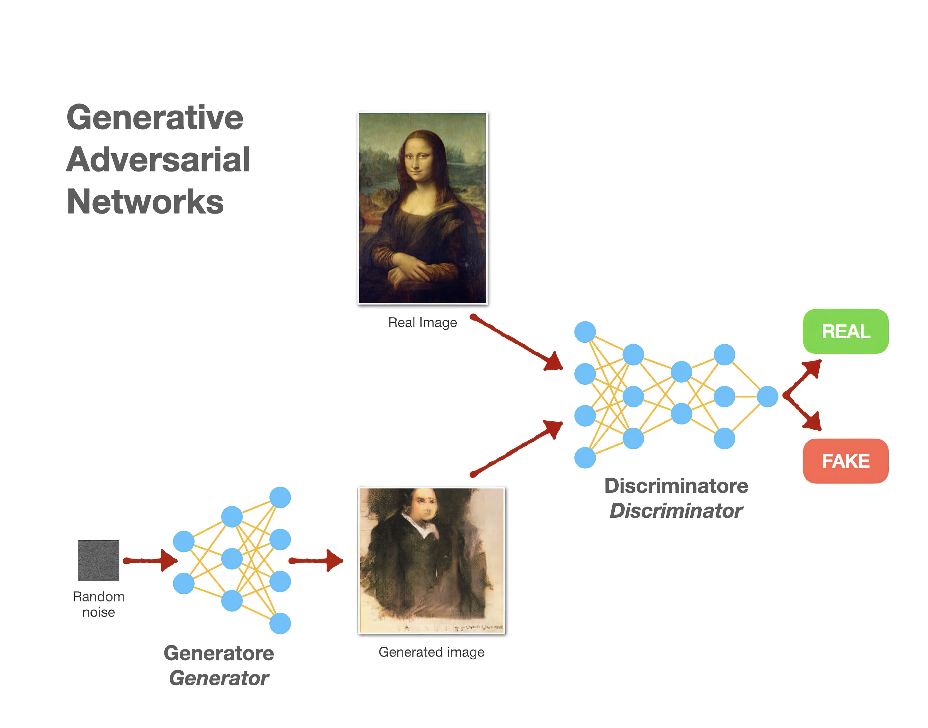
\includegraphics[scale=0.6]{figures/GANs-ex-art.png}
  \caption{Example of a GAN architecture}
  \label{fig:GAN architecture}
\end{figure}

\subsubsection{GAN structure and training}
\noindent A GAN has a similar structure to that of an autoencoder, where the discriminator serves as the encoder. However, instead of producing an encoded representation, it only outputs whether the input is real or fake. On the other hand, the generator acts like the decoder and takes in random data from the latent space, learning to generate new content that can trick the discriminator into thinking it is real. Both the generator and discriminator are trained in a competitive manner, with the generator striving to maximise the error of the discriminator and the discriminator trying to minimise it.\\

\noindent The generator and the discriminator are two distinct deep neural networks. The generator is a function G that takes a random noise vector $z$ as input and maps it to the data space, producing a set of synthetic samples. These samples are fed into the discriminator network D, together with the real samples $x$. This network outputs a single scalar that represents the probability that the sample came from the real data distribution rather than the synthetic data distribution. Therefore, the discriminator learns to use traditional supervised learning techniques, dividing inputs into two classes (real or fake).

\noindent The GAN training process is a two-player that involves updating the weights of the generator and discriminator networks using gradients computed from the loss function. The loss function, also called cost function, in a GAN is designed to quantify the difference between the generated data and the real data. The objective is to find the balance between the generator and discriminator losses, where the generator loss represents the ability of the generator to produce realistic synthetic data and the discriminator loss represents the ability of the discriminator to distinguish between real and fake data.

\noindent There are several cost functions that may be used, and they usually differ in terms of the cost function used for the generator.

\noindent The basic loss function used in GAN is the binary cross-entropy:
\begin{equation}
\label{eq:binariCross-entropy}
L(\hat{y}, y) = [y \times \log (\hat{y}) + (1-y)\times \log (1-\hat{y})]
\end{equation}
where $y$ represents the original data and $\hat{y}$ the generated one. In training, the discriminator assumes $y=1$ for real data, while for the generated data it is set: $\hat{y} = D(x)$. Substituting this information in equation~\ref{eq:binariCross-entropy} the discriminator loss can be obtained: 
\begin{equation}
    L(D(x),1)=\log(D(x))
\end{equation}
For the generator's output data, it is assumed that $y = 0$, because it outputs fake data, and $\hat{y} = G(D(z))$ for the generated data, where $z$ is a random noise vector sampled from a noise distribution $p_z(z)$ (e.g., uniform or Gaussian distribution). Therefore, the loss for the generator is:
\begin{equation}
    L(D(G(z)),0) = \log(1 - D(G(z)))
\end{equation}
To obtain the total discriminator loss the two equations above have to be combined and maximised:
\begin{equation}
L^{(D)}=\max [\log (D(x)) + \log(1-D(G(z)))]
\end{equation}
The generator has to fool the discriminator, hence it has the opposite goal, therefore to obtain its loss function its minimum has to be calculated:
%is obtaining by computing the minimum:
\begin{equation}
L^{(G)}=\min [\log (D(x)) + \log(1-D(G(z)))]
\end{equation}
The loss function is designed to encourage the generator to produce realistic synthetic data and the discriminator to distinguish between real and fake data with high accuracy.

\noindent The interdependence of each player's cost on the other player's parameters, along with the lack of control over the other player's parameters, makes this scenario more accurately described as a game rather than an optimisation problem. 
%The solution of this game is the \textit{Nash equilibrium}.
The loss function in a GAN is an important component of the training process, as it determines the quality of the generated data and the ability of the discriminator to accurately distinguish between real and fake data. 
\\
\noindent The training process of GANs is a zero-sum game in which the objective function of this minimax optimisation problem is:
\begin{equation}
\label{eq:minimax obj function}
    \min \max V(D,G) = \min_G \max_D \mathbb{E}_{x \sim p_{data}(x)}[\log D(x)]+\mathbb{E}_{z \sim p_z(z)}[\log (1- D(G(z)))]
\end{equation}
where $x$ is a real image from the true data distribution $p_{data}$, and $z$ is a noise vector sampled from the noise distribution $p_z$. $\mathbb{E}_x$ and $\mathbb{E}_z$ denote the expected log likelihood from the different outputs of both real and generated images.

\noindent In training a GAN, it is important to ensure that both the generator and discriminator models are developed in a balanced manner. The success of the GAN largely depends on the alignment of the real and generated distributions, and this can only be achieved if neither of the models is overly dominant.
In addition to train the generator and the discriminator, the errors on their outputs are backpropagated into the models as gradients of the loss functions, as shown in Fig.~\ref{fig:GAN architecture w loss}. These loss functions are used to guide the learning process and ensure that the generator produces high-quality samples.
\begin{figure}[!ht]
\centering
  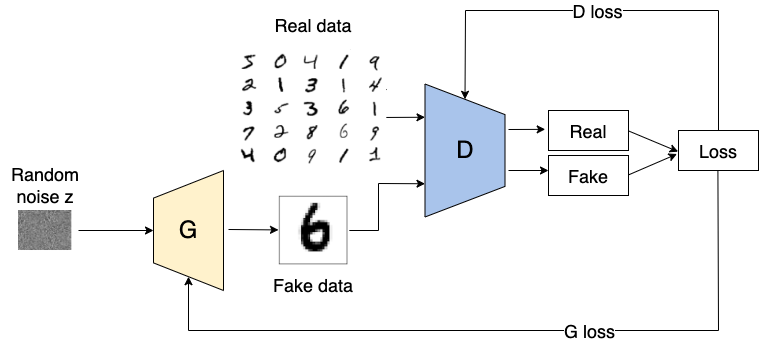
\includegraphics[scale=0.4]{figures/gan-architecture.png}
  \caption{Architecture of a GAN. The generator and the discriminator are synchronously trained.}
  \label{fig:GAN architecture w loss}
\end{figure}
If the discriminator is too good at identifying fake versus real images early in the training process, the generator may struggle to produce convincing fake images, making it difficult for the two models to improve. If the generator is successful in fooling the discriminator, the loss will backpropagate through the discriminator network to improve its performance. On the other hand, if the discriminator effectively distinguishes between fake and real samples, the loss will backpropagate through the generator network to improve its ability to generate samples that are similar to real samples.
The update rules for the discriminator and the generator are shown in equations~\ref{eq:update rule discriminator} and~\ref{eq:update rule generator} respectively. The weights of each model are represented by $\theta_d$ and $\theta_g$, respectively, and $m$ represents the total number of samples in a batch used to test the models before updating them. Algorithm~\ref{alg:training optimisation} optimises Eq.~\ref{eq:minimax obj function} as show by~\cite{GANGoodfellow}.

\noindent From a mathematical point of view, if the discriminator gets too good at identifying the samples, this may increase the divergence between the generated expected distribution. In case the generated and the real distributions become too diverse or do not overlap, then the generator will suffer from vanishing gradient loss.

\noindent The vanishing gradient problem is a critical issue in training deep neural networks. The problem occurs when the gradients of the parameters with respect to the loss become extremely small, making it difficult for the optimizers to update the parameters of the network effectively since they do not have any effect on the training model. The vanishing gradient problem can lead to slow convergence or complete failure of the training process. 
One possible solution to this problem is to use the Wasserstein GAN architecture.\\

\begin{algorithm}
\caption{Minibatch stochastic gradient descent training of generative adversarial nets. The number of steps to apply to the discriminator, $k$, is a hyperparameter.}
\begin{algorithmic}
\label{alg:training optimisation}
\For {number of training iteration}
    \For {$k$ steps }
         \Statex\begin{itemize}
         \setlength{\itemindent}{.2in}
             \item Sample minibatch of $m$ noise samples $\{ \mathbf{z}^{(1)}, ..., \mathbf{z}^{(m)}\}$ from noise prior $p_g(\mathbf{z})$
             \item Sample minibatch of $m$ examples $\{ \mathbf{x}^{(1)}, ..., \mathbf{x}^{(m)}\}$ from data generating distribution $p_{pdata}(x)$.
             \item Update the discriminator by ascending its stochastic gradient: 
                \begin{equation}
                \label{eq:update rule discriminator}
                    \nabla_{\theta_d}\frac{1}{m}\sum_{i=1}^m [ \log D(x^{(i)}) + \log (1 - D(G(z^{(i)})) ]
                \end{equation}
         \end{itemize}
    \EndFor
    \begin{itemize}
     \setlength{\itemindent}{.2in}
        \item Sample minibatch of $m$ noise samples $\{ \mathbf{z}^{(1)}, ..., \mathbf{z}^{(m)}\}$ from noise prior $p_g(z)$. 
        \item Update the generator by descending its stochastic gradient:
        \begin{equation}
        \label{eq:update rule generator}
            \nabla_{\theta_g}\frac{1}{m}\sum_{i=1}^m [ \log (1 - D(G(z^{(i)})) ]
        \end{equation}
    \end{itemize}
\EndFor
\end{algorithmic}
The gradient-based updates can use any standard gradient-based learning rule.
\end{algorithm}

\newpage
\noindent The goal is to make the expected and generated distribution match as closely as possible. 
The GAN continues this process back and forth until an equilibrium is reached between the generator and discriminator loss. Over time, the two networks learn from each other and converge to a state where the generator produces samples that are almost indistinguishable from real data, and the discriminator is able to correctly identify which samples are real and which are fake with high accuracy.

\noindent This basic design is referred to as the Vanilla GAN, as it represents the original model from which more advanced GAN architectures have evolved, yet still retaining the two key components of the GAN structure.
% ************************************
% ************************************
\subsection{Wasserstein-GAN}
\label{sec:wgan}
The Wasserstein-GAN, also known as WGAN, is a variant of the Vanilla GAN and it was introduced by Arjovsky et al. in 2017~\cite{wgan}. WGAN aims to improve the generator model's capability of approximating the data distribution of a given training dataset by introducing a different training mechanism. 
Instead of using a discriminator to classify the generated images as real or fake, WGAN uses a critic that scores the authenticity of an image. It uses the Wasserstein distance (also known as Earth-Mover's distance), which is a metric that quantifies the minimum cost of moving mass from one distribution to another to convert the source distribution $q$ to the target distribution $p$. It is used to measure the distance between the distribution of real data and the distribution of generated data.

\noindent In WGAN, the discriminator is trained to be a function that outputs a scalar value instead of a probability, and the generator is trained to minimise the Wasserstein distance.

\noindent One formulation for the Wasserstein distance is:
\begin{equation}
    \label{eq:waaserstein distance}
    W(\mathbb{P}_r , \mathbb{P}_g)= \sup_{f \in \mathcal{F}} \mathbb{E}_{x\sim \mathbb{P}_r}[f(x)] - \mathbb{E}_{x \sim \mathbb{P}_g}[f(x)]
\end{equation}
where $\mathcal{F}$ is defined as the set of 1-Lipschitz functions, which are those satisfying $\|f\|_L \leq 1$ where $\| \cdot \|_L$ represents the Lipschitz norm.

\noindent The WGAN objective function can be formulated as:
\begin{equation}
    \min_G \max_{D \in \mathcal{F}} \mathbb{E}_{\mathbf{x} \sim \mathbb{P}_r} [D(\mathbf{x})] - \mathbb{E}_{\Tilde{\mathbf{x}} \sim \mathbb{P}_g}[D(\Tilde{\mathbf{x}})]
\end{equation}
where $\mathbb{P}_r$ and $\mathbb{P}_g$ are respectively the real and generated distribution, $\Tilde{\mathbf{x}} = G(z)$ with $z \sim p(z)$.
The above formulation needs the critic to be 1-Lipschitz. This condition is ensured by clipping the weights $\mathbf{W}$ of the discriminator to be within a compact range of $[-c ,c]$, where $c$ is a user-defined hyper-parameter. Specifically, each weight $w_{i,j}$ is clipped to this range.\\
%

\noindent \textbf{WGAN-GP}

\noindent One step towards stable training of GANs is made by WGAN, however, it may still generate inadequate samples or not converge. The cause of such issues is frequently attributed to the utilisation of weight clipping in WGAN, which enforces a Lipschitz constraint on the critic and can result in undesirable behaviour, for example, the convergence of a very deep WGAN critic may often fail. Therefore, to address this issue an alternative to weight clipping has been proposed by~\cite{wgan-gp} to ensure smooth training, which is the Wasserstein GAN with Gradient Penalty (WGAN-GP).
The WGAN-GP method replaces weight clipping with a gradient penalty, introducing an extra loss term that encourages the discriminator to have a gradient with a norm that is near $1$. The resultant optimization problem is given by: 
\begin{equation}
    L = \mathbb{E}_{\Tilde{\mathbf{x}}\sim \mathbb{P}_g}[D(\Tilde{\mathbf{x}})] - \mathbb{E}_{\mathbf{x}\sim \mathbb{P}_r}[D(\mathbf{x})] + \lambda \mathbb{E}_{\hat{\mathbf{x}}\sim \mathbb{P}_{\hat{\mathbf{x}}}} [( \| \nabla_{\hat{\mathbf{x}}} D( \hat{\mathbf{x}}) \|_2 - 1)^2]
\end{equation}
where the first two terms are the original critic loss of the WGAN, while the last term is the gradient penalty, in which $\lambda$ defines the gradient penalty coefficient, $\hat{x}$ is a random sample along the straight line between real and generated samples and $p_{\hat{x}}$ is the distribution of $\hat{x}$.
% ************************************
% ************************************
\subsection{ProGAN}
\label{sec:proGAN}
ProGAN, short for Progressive Generative Adversarial Network, is a deep learning model that was developed to generate high-resolution, photorealistic images. It was introduced by Karras et al. in 2017~\cite{ProGAN}, it is a type of generative model, which means that it can generate new, synthetic images based on the data it is trained on.

\noindent The main idea behind ProGAN is to use a series of generators and discriminators to generate high-resolution images incrementally, starting from low-resolution images (e.g. 4×4) and gradually increasing the resolution until a high-resolution image is obtained (e.g. 1024×1024). This approach is called progressive growing, and it allows the network to learn the finer details of an image in an incremental manner. The generator starts with a random noise input and generates an image with low resolution, which is then evaluated by the discriminator. The discriminator determines whether the generated image is real or not and provides feedback to the generator, allowing it to improve. \\

\noindent One of the benefits of ProGAN is that it generates high-resolution images that are photorealistic, which makes it useful for various applications. Additionally, ProGAN is trained on large datasets, which means that it can create diverse and varied images.
Another advantage of ProGAN is its ability to produce images at different resolutions, which allows for a level of control over the generated images.

\noindent Some drawbacks of the progressive growth method in a GAN are the prolonged training time involved in constructing subsequent models at higher resolutions, the need for extra resources in terms of data preparation and storage, and of course the non-negligible computational time.
%
%
%
\subsection{Evaluation metric}
\subsubsection{xCos}
\label{sec:xcos}
The state-of-the-art face verification models employ a methodology that involves extracting deep features from a pair of face images and subsequently computing the cosine similarity or the L2-distance of the paired features. The determination of whether the two images are of the same person is based on whether the similarity value exceeds a pre-defined threshold value. However, the approach proposed in the paper “xCos: An Explainable Cosine Metric for Face Verification Task”~\cite{xCos} offers a distinctive approach in which the verification result is obtained by the integration of the local similarity map and the attention map. It is based on the insight that humans tend to compare different facial features to determine whether two face images belong to the same individual. \textit{xCos} leverages this understanding to evaluate the similarity of facial features between two images. It is built using a grid-based feature extraction approach, in which each face image is divided into multiple local regions. The facial features of each local region are then extracted and compared with the features of the corresponding regions in the other image. The resulting similarities are then aggregated across all the local regions to compute a final similarity score. It also includes an attention mechanism that identifies the specific facial features that contribute the most to the similarity score. This attention mechanism allows for a more interpretable and explainable verification result, as it highlights the specific facial features that the model is prioritising. \\

\noindent The proposed architecture, showed in Fig.~\ref{fig:xCos architecture}, for face recognition consists of a modified CNN backbone and two branches for \textit{xCos} and identification. 
\begin{figure}[!ht]
\centering
  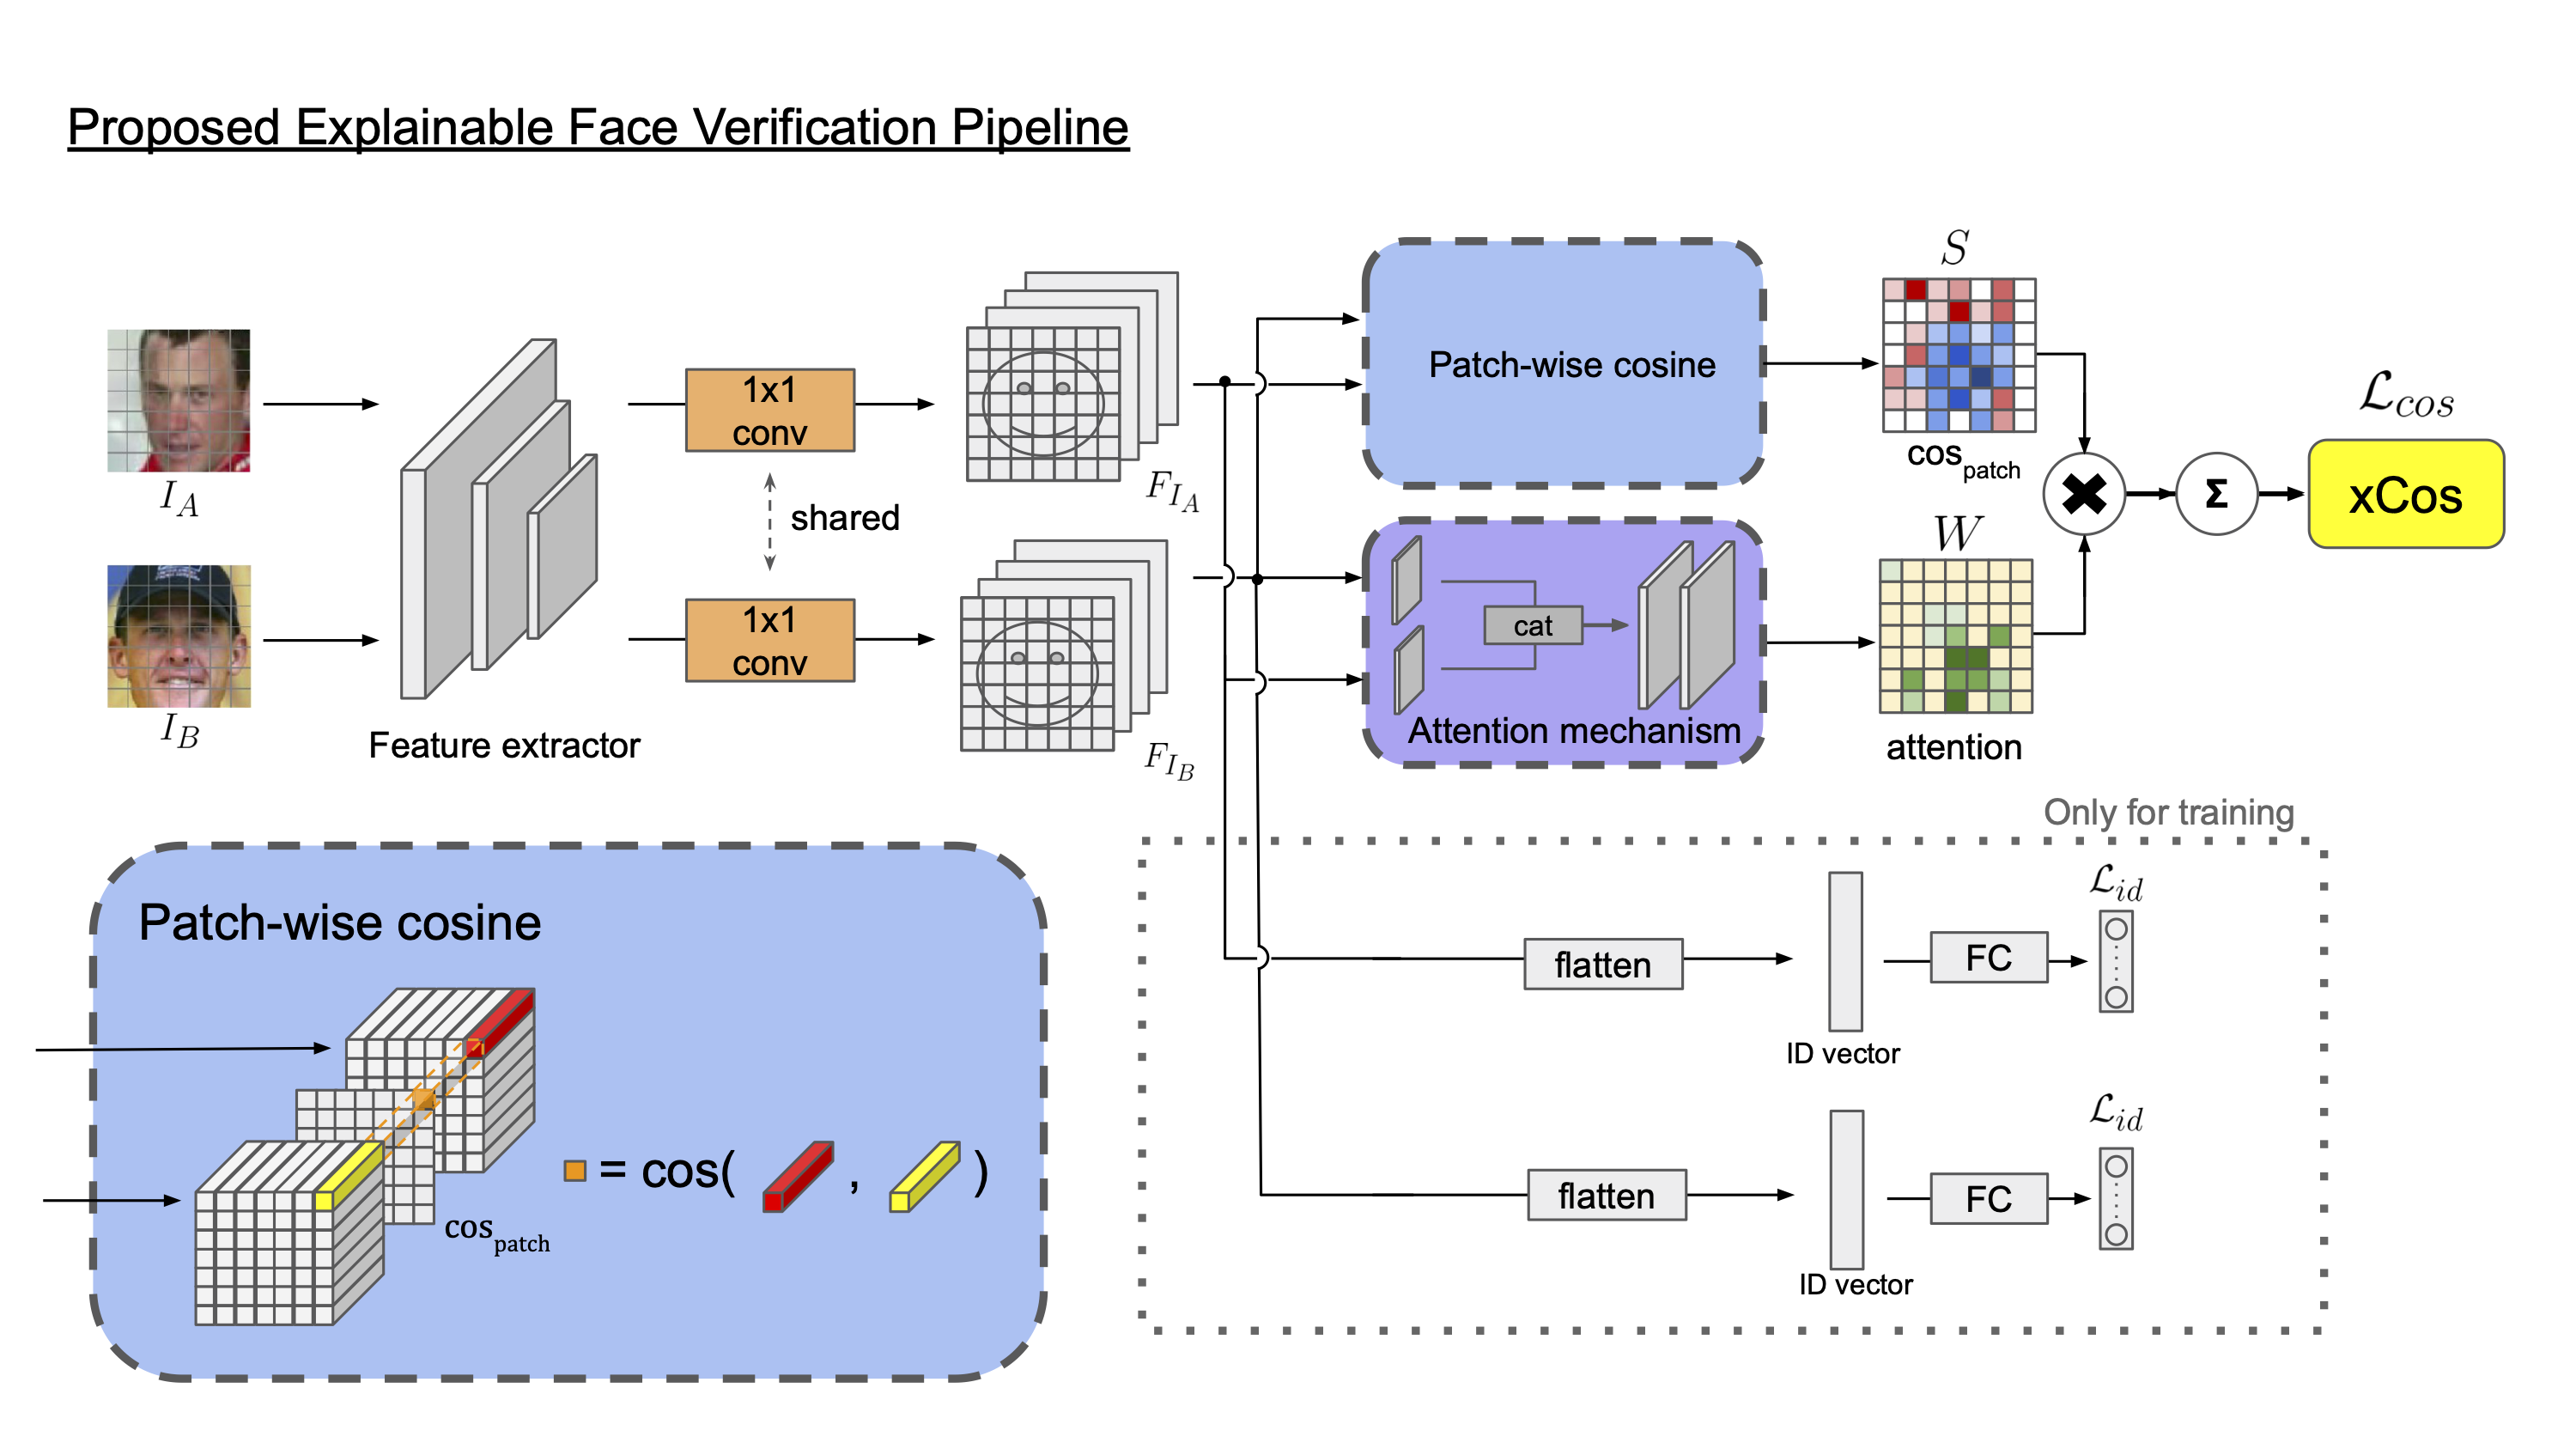
\includegraphics[scale=0.5]{figures/xCos-architecture.png}
  \caption{Example of the xCos architecture taken from~\cite{xCos}}
  \label{fig:xCos architecture}
\end{figure}
The primary responsibility of the CNN backbone is to extract facial features for each identity. To preserve the position information of each feature point, the final flatten and fully-connected layers of the backbone, such as ArcFace~\cite{arcface2018} or CosFace~\cite{cosFace}, are replaced with a \num{1} by \num{1} convolution.
On the xCos branch, to compute a patched cosine map $S$ ($\cos_{patch}$), the two feature maps of compared images are element-wise evaluated using cosine similarity.
At the same time, an attention weight map $W$ is generated using the attention mechanism based on the two feature maps. The final xCos similarity value is achieved by performing a weighted sum of the patched cosine map $S$, using the attention weight map $W$.

\noindent The xCos branch is trained using cosine similarity computed by another face recognition model, such as ArcFace. The identification branch flattens the extracted feature and feeds it into another fully connected layer for predicting the identity. The training is stabilised by using a common face recognition loss, such as the one used in ArcFace, which is denoted as $\mathcal{L}_{ID}$.
 % CAP 2
\newpage
\section{Dataset building}
\label{section:datasetChapter}
Since the objective of this thesis is to generate a realistic photo of a face starting from a handmade sketch, a neural network had to be trained on a large dataset of face images and their corresponding sketches. However, finding such a dataset is not easy. Online there is available the \href{http://mmlab.ie.cuhk.edu.hk/archive/facesketch.html}{CUHK dataset} (The Chinese University of Hong Kong), it is a collection of images and annotations used for various computer vision and machine learning tasks, such as image classification, object detection, and face recognition. The specific content and size of the CUHK dataset may vary depending on the source. It is often used as a benchmark for evaluating and comparing the performance of different algorithms in various computer vision tasks. The dataset includes the CUHK Face Sketch FERET Database (CUFSF) which is composed of a pair of images with both a photo of a face and a sketch of it. Each face in the database includes an artist-drawn sketch based on a photo that was taken with the individual in a neutral expression, under normal lighting conditions, and in a frontal pose. This database is made for the purpose of researching face sketch synthesis and face sketch recognition. Unluckily, it does not contain enough images, and it requires data augmentation techniques in order to use it.  \\
Another dataset available online is the \href{https://github.com/NVlabs/ffhq-dataset}{FFHQ} (Flickr-Faces-HQ) dataset, which is a large-scale, high-quality dataset of face images, created to advance research in generative models and computer vision. The dataset contains $70,000$ high-resolution (1024×1024) images of diverse human faces, each with different poses, lighting, expressions, and ethnicities. Since it is a very large dataset, it can be used to create the needed dataset composed of the pairs of sketches and photos, but it requires some image processing techniques in order to obtain the sketches.

\noindent The challenge here is to find a technique to transform an image into a sketch. The idea is to extract the face contours using an edge detection technique while preserving the essential details of the face and making the extracted  a hand-drawn sketch appearance

\noindent To achieve these results, two approaches were considered to build the dataset. The first approach involves using the \href{https://github.com/vijishmadhavan/ArtLine}{Artline} network and the Learning to Simplify network \cite{SketchSimplify}. The second approach involves using an extended difference of Gaussian (XDoG) edge detector \cite{xdog} and the Learning to Simplify network.
In order to produce the desired results, both approaches need to be carefully analysed and compared. In this way, the most appropriate approach can be chosen and further developed to create a realistic handmade sketch. 
Now will follow an introduction of the above approaches before discussing how they have been used to reach the final goal.

\subsection{Artline}
Artline is a deep neural network designed specifically to turn photographs into line art drawings. It is a recent project developed by a developer interested in generative modelling, that follows the discoveries found by Jason Antic, another developer, in his \href{https://github.com/jantic/DeOldify}{DeOldify} project, utilising advancements and tools developed by the team at Fast.ai. Artline, as DeOldify, is based on a self-attention GAN (SAGAN) that is progressively resized to achieve a desired resolution. SAGAN was introduced in a 2018 research paper by Zhang et al.\cite{SaGAN} and has since been applied to a wide range of image generation tasks, including facial image synthesis, artistic image generation, and more. The results have been very promising, with SAGAN producing high-quality and highly detailed images that are comparable to those produced by state-of-the-art methods. \\
The self-attention mechanism allows the generator network to weigh the contribution of different parts of an image in generating the final result. This allows the network to focus on important features of the image and produce more accurate results. Additionally, the use of self-attention also allows the network to better capture the relationships between different parts of the image, resulting in more coherent and visually appealing images.
Artline has been trained on the APDrawing dataset, which is a dataset obtained from another generative neural network able to generate high-quality sketch drawings from a given image, called APDrawingGAN \cite{APDrawingGAN}. The APDrawingGAN is an innovative GAN-based architecture that has the capability to generate professional-level artistic portraits. It uses a combination of a global network and local networks, which allows for dedicated drawing strategies to be learned for specific facial features. This leads to a more precise and accurate portrayal of facial features in the generated drawings. To train APDrawingGAN, a unique artistic drawing dataset was constructed, containing high-resolution portrait photos and corresponding professional artistic drawings. The results of extensive experiments and a user study demonstrate that APDrawingGAN produces significantly better artistic drawings than existing methods. Since the results obtained by the authors using this dataset were good only in the case of ID photos, the authors combined this dataset with an Anime sketch dataset to obtain good results also with other kinds of pictures.

\subsection{Learning to simplify}
Learning to Simplify is a model which consists of a fully convolutional network (FCN) to learn the mapping between rough sketches and clean drawings. The technique of simplifying rough sketches utilises Convolutional Neural Networks (CNNs) to simplify the image. Through a series of convolution operations, the sketch lines are grouped, and a simplification is directly produced. The CNNs are trained using a unique dataset of rough sketches and their corresponding simplifications, which the authors have created. This data-driven method has several benefits. Firstly, the model automatically learns the necessary heuristics for sketch simplification from the training data. Secondly, convolution operations can be executed efficiently on GPUs, resulting in processing times of less than a second for most images. In contrast to typical CNN architectures, which utilise fully connected layers, their approach uses solely convolutional layers. These sparse connections allow their CNN to process images of varying resolutions and aspect ratios with ease. The results of the study show that the FCN is able to produce high-quality clean drawings from rough sketches with remarkable accuracy.
\begin{figure}[h!]
\centering
  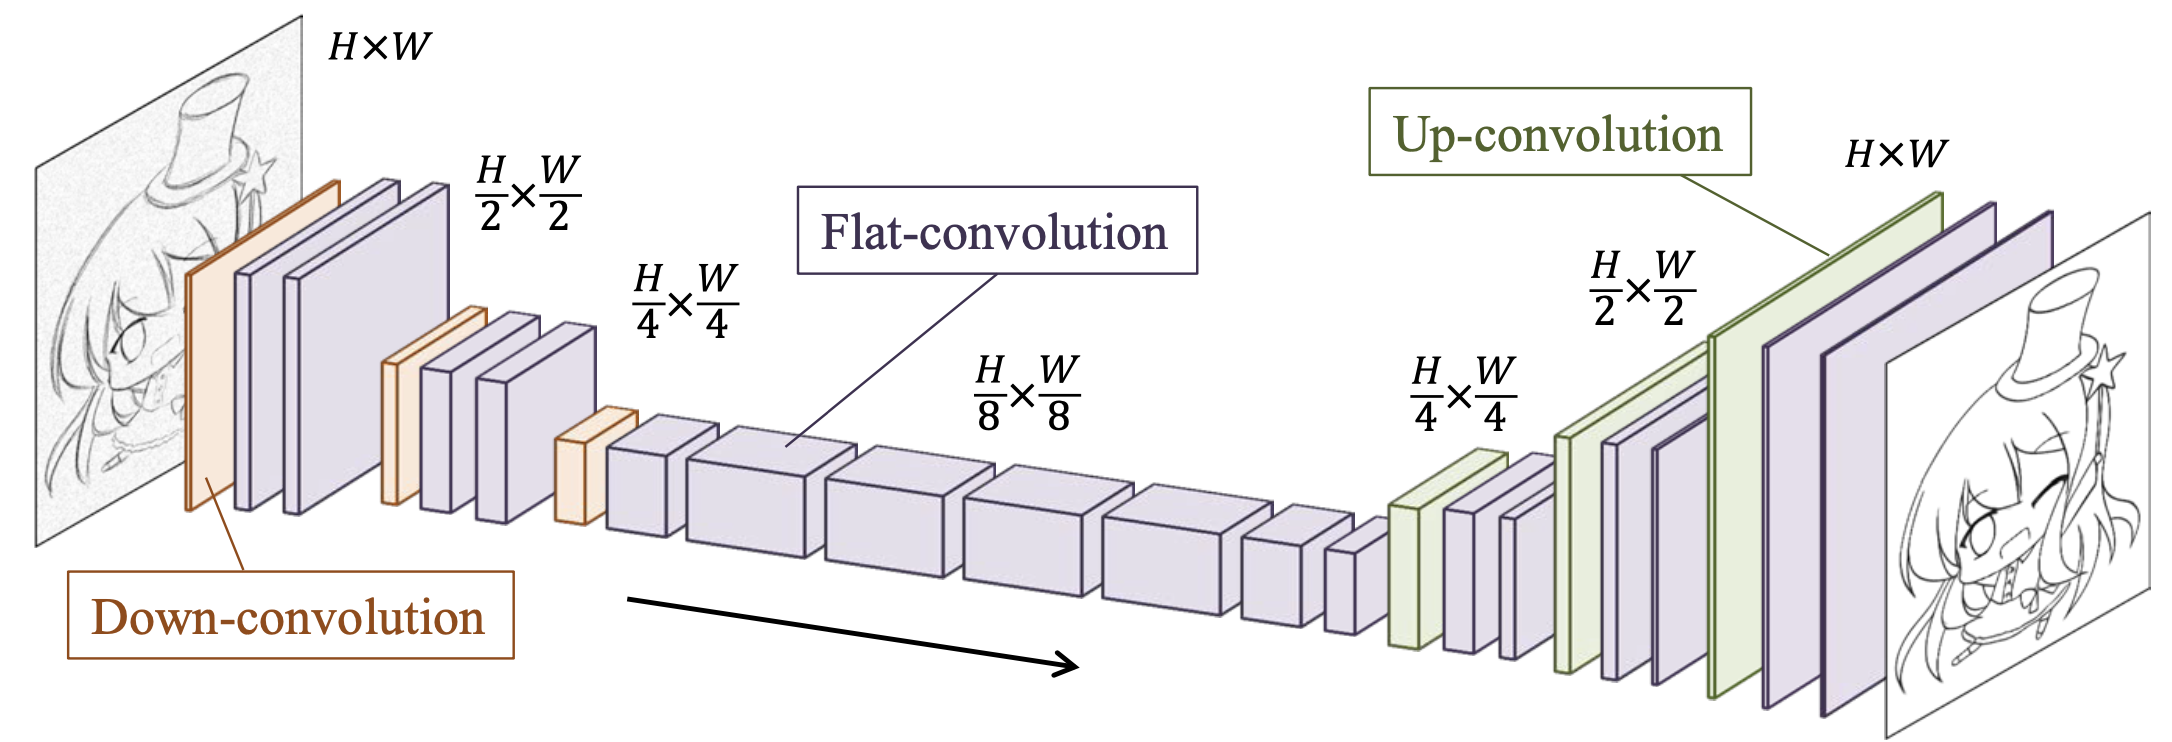
\includegraphics[scale=0.35]{figures/learnToSimplifyArchitecture.png}
  \caption{Learning to Simplify architecture. Image taken from \cite{SketchSimplify}}
  \label{fig:Learning to Simplify architecture}
\end{figure}
\\
The model has three main components: an encoder that compresses the image, a processing unit that extracts the critical lines, and a decoder that converts the simplified representation back into a greyscale image of the same resolution as the input (Figure \ref{fig:Learning to Simplify architecture}). All these components use convolutional layers for their processing.


\noindent The model uses a down- and up-convolution architecture that may look like simple filter banks. However, the model has a larger number of channels in lower-resolution parts, such as 1024 channels when the size is 1/8, to ensure that the necessary information for clean lines is carried through. The model uses padding in its convolutional layers to ensure the output is the same size as the input when a stride of 1 is used. Instead of pooling layers, they used convolutional layers with a higher stride to lower the resolution from the previous layer. To increase the resolution and ensure that the output of the model has the same dimensions as the input, they used fractional strides.
Overall, the model leverages the ability of CNNs to learn and extract essential information, making it an effective solution for sketch simplification.
The Learn to simplify model has been trained by the authors using pairs of rough and simplified sketches representing the input and the target, respectively.
An example of the results that can be obtained with this approach can be seen in fig. \ref{fig:Learning to Simplify results}.
\begin{figure}[htbp]
\centering
  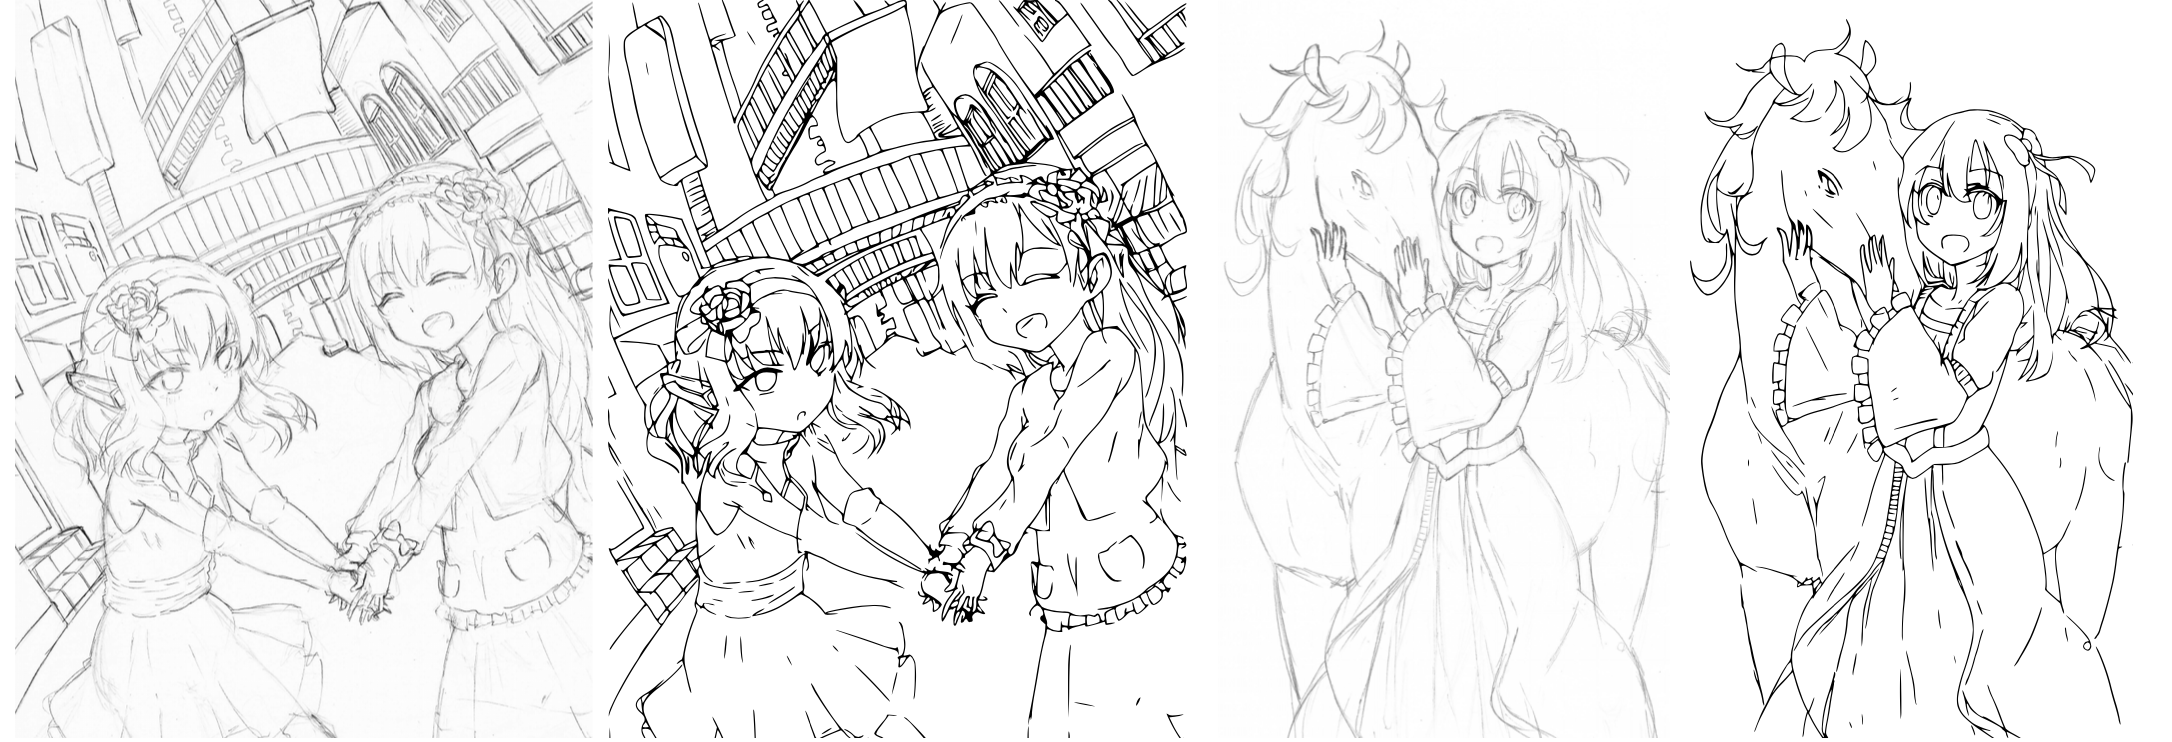
\includegraphics[scale=0.25]{figures/learnToSimplify-results-paper.png}
  \caption{Figure from \cite{SketchSimplify}} showing the results of Learning to Simplify approach.
  \label{fig:Learning to Simplify results}
\end{figure}

\subsection{Extended Difference of Gaussian (XDoG)}
The Extended Difference of Gaussian (XDoG) is an edge detector operator based on the Difference of Gaussian (DoG). The Difference of Gaussian is based on the idea that edges in an image correspond to rapid changes in intensity, which can be detected by subtracting two images that have been smoothed with different Gaussian kernels. It can be used to increase the visibility of edges and other features in digital images.
The capacity of the DoG operator to extract information about the edges in the image can be explained by considering the Gaussian filter from a signal processing point of view. The Gaussian filter is defined as: 
\begin{equation}
    G_{\sigma}(x)=\frac{1}{2\pi \sigma^2}e^{-\frac{x^2}{2\sigma^2}}
\end{equation}
where $x$ refers to a two-dimensional coordinate, and $\sigma$ represents the standard deviation of the Gaussian distribution in the spatial domain. It is a low-pass filter which attenuates or eliminates high frequencies. The difference between the two Gaussian with different is equivalent to a subtraction between a blurred version of the original image and a less blurred version of it, and it is defined as: 
 \begin{equation}
     D_{\sigma, k}(x)=G_{\sigma}(x)-G_{k\sigma}(x) \approx -(k-1)\sigma^2 \nabla ^2 G
 \end{equation}
where the standard deviations of these Gaussian filters determine the scale at which edges are detected, with larger standard deviations detecting larger edges.
This difference is a band-pass filter which attenuates all frequencies between the cut-off frequencies of the two Gaussians and results in a new image that highlights regions of the original image where the intensity changes rapidly.

\noindent The XDoG approach is inspired by biological models proposed by Young and others \cite{GaussianDerivativeModel}, which were based on the DoG model. Winnem$\ddot o$ller et al. \cite{RealTimeVideoAbstraction} extended the DoG model to allow for greater control over the inhibitory effect of the larger Gaussian, which is allowed to vary, resulting in a more advanced edge detection technique with the following equation:
\begin{equation}
    D_{\sigma, k,\tau}(x)=G_{\sigma}(x)-\tau \cdot G_{k\sigma}(x)
    \label{eq:xdog}
\end{equation}
 This allows for more fine-grained control over the output, resulting in more precise edge detection and image stylization. In particular, it is possible to achieve a wider range of stylistic effects using the following continuous ramp function:
 \begin{equation}
     T_{\epsilon, \varphi}(u) = 
     \begin{cases}
        1 & u \ge \epsilon \\
        1+ \tanh (\varphi \cdot (u-\epsilon)) & \mbox{otherwise}
    \end{cases}
\label{eq:xdog1}
 \end{equation}
Equations \ref{eq:xdog} and \ref{eq:xdog1} taken together is referred to as the XDoG filter $T_{\epsilon, \varphi}(D_{\sigma, k, \tau }*I)$ for a given image $I$. 

\noindent There are a lot of known edge detectors that can be applied to find the edges of objects present in an image, and they have their advantages and disadvantages (as shown in \cite{xdog}). Since the objective was not only to extract contours but also to obtain something that looks like a sketch done by an artist, not all the edge detectors that are known could be applied. 

\noindent As can be seen from figure \ref{fig:xdog-paperComparison}, some edge detectors work well in extracting edges, like the Sobel filter and the Canny edge detector, but the results obtained are not satisfactory from an artistic point of view. Hence, the XDoG operator has been chosen since it satisfies the final purpose.

\begin{figure}[htbp]
\centering
  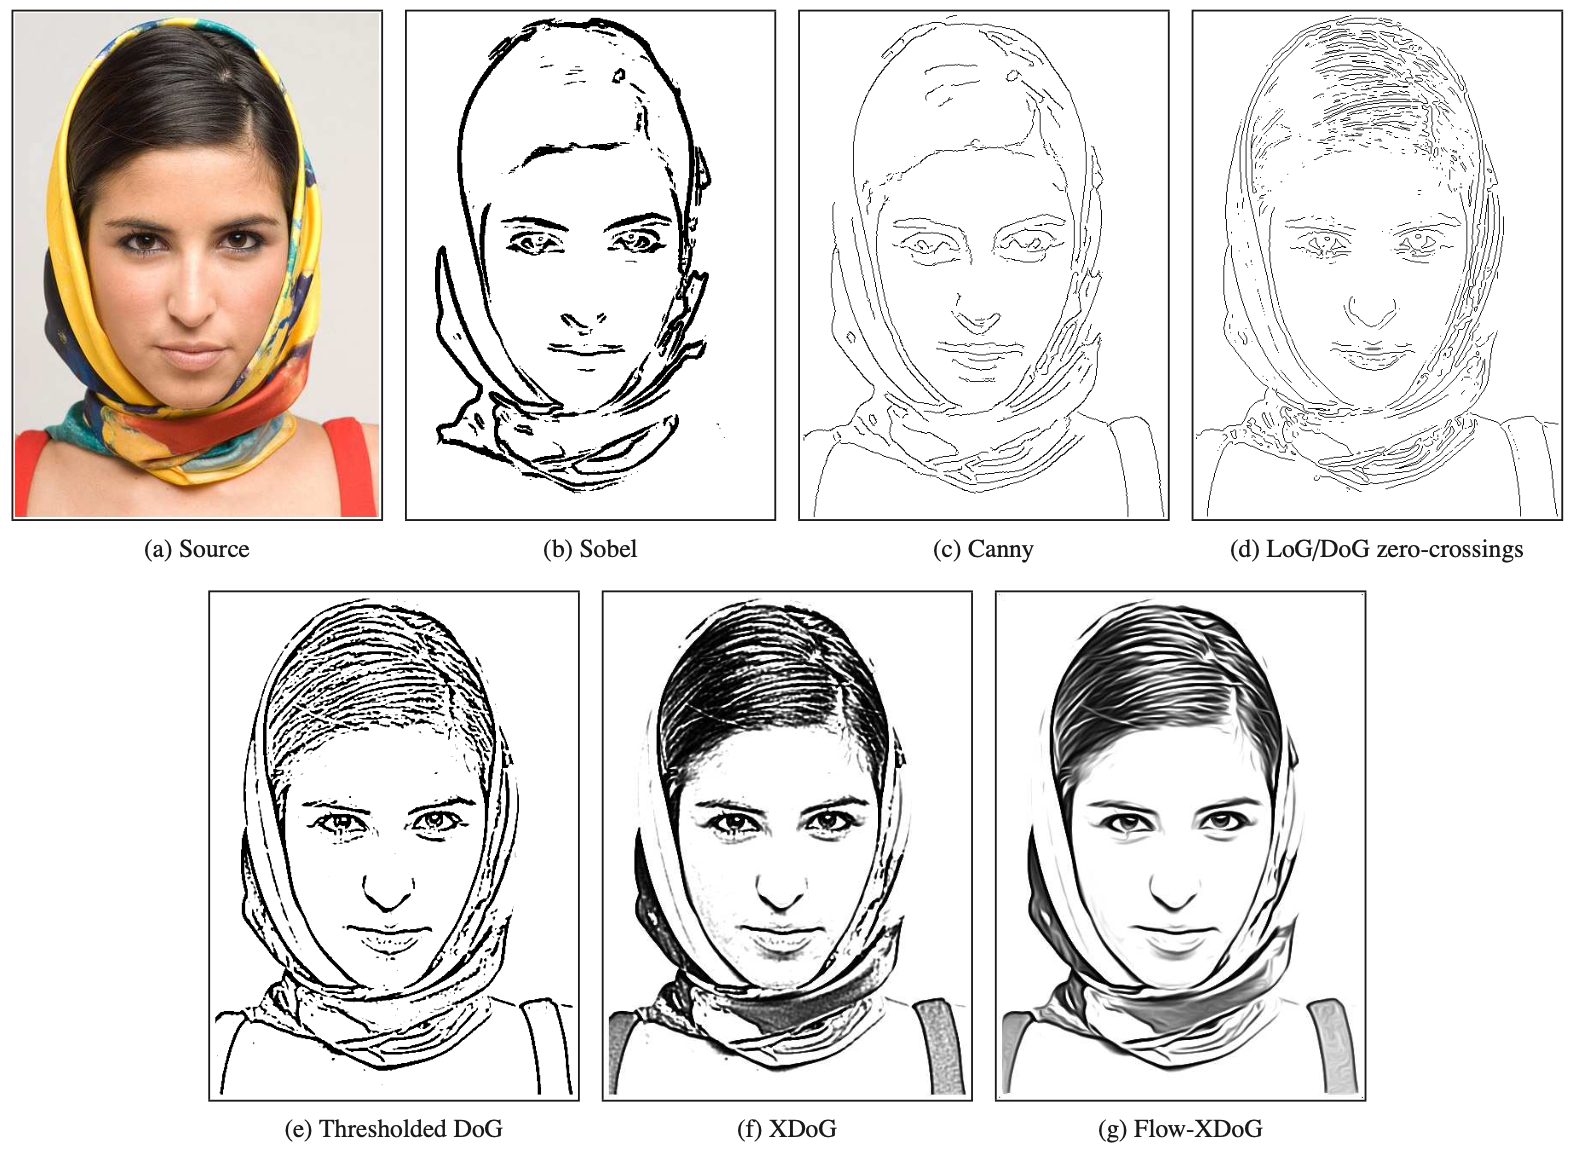
\includegraphics[scale=0.4]{figures/comparisonOfEdgeDetectors.png}
  \caption{Figure taken from \cite{xdog} in which there is a comparison between different known edge detection techniques.}
  \label{fig:xdog-paperComparison}
\end{figure}

\subsection{Implementation (??)}
In order to achieve the needed dataset, the following approaches have been followed:
\begin{enumerate}
    \item Artline network + Learning to Simplify network
    \item extended difference of Gaussian (XDoG) edge detector + Learning to Simplify network
\end{enumerate}
The first idea was to take the images and extract the contours using Artline neural network and then simplify the result by removing some lines from the obtained sketch.
The results obtained applying only Artline can be seen in Fig. \ref{fig:artlineRes}, they are very good and give the impression that they are made by an artist. Nevertheless, they do not seem like sketches made with a pencil because all the people's hair and facial hair are coloured in black. Therefore, there was a need to try to simplify these images, by applying sketch simplification which can be obtained thanks to Learning to Simplify. This network can be used with four different models that are available and can be used to achieve different results.
\noindent The models are:
\begin{itemize}
    \item a model obtained from training the network using only MSE loss
    \item a model obtained from training the network using MSE and GAN loss
    \item a model for pencil drawing generation based on an artist with a dirty and faded pencil style (pencil1)
    \item model for pencil drawing generation based on an artist with a clearer overlay pencil style (pencil2)
\end{itemize}
\begin{figure}[htbp]
    \centering
    \subfloat[][\emph{Original imag}]
    {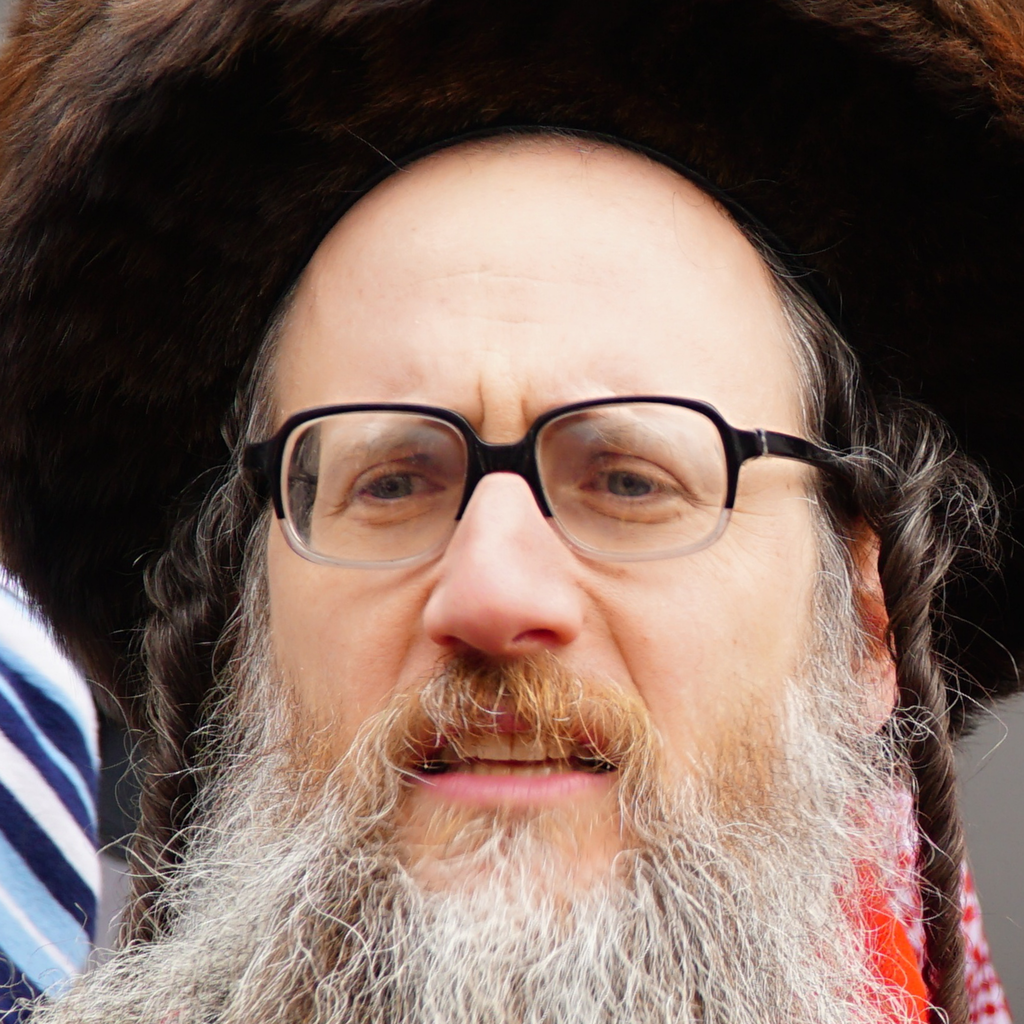
\includegraphics[width=.19\textwidth]{figures/66000.png}} \quad
    \subfloat[][\emph{Artline's output}]
    {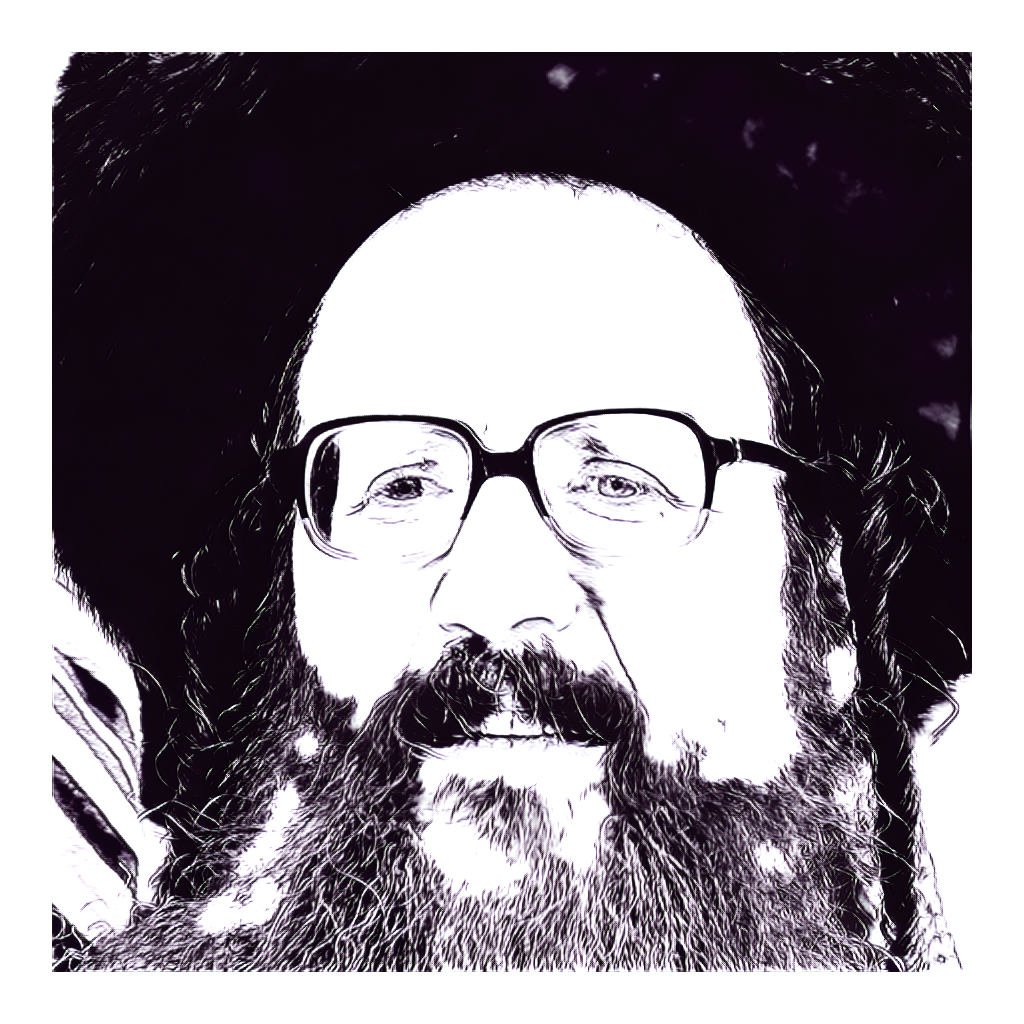
\includegraphics[width=.2\textwidth]{figures/66000Artile.png}} \\
    \subfloat[][\emph{Original image}]
    {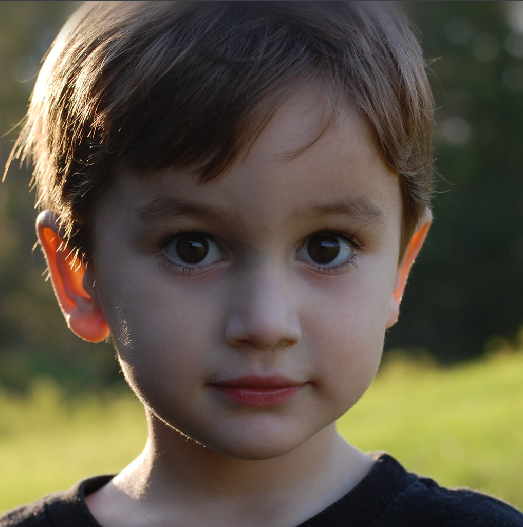
\includegraphics[width=.19\textwidth]{figures/66006.png}} \quad
    \subfloat[][\emph{Artline's output}]
    {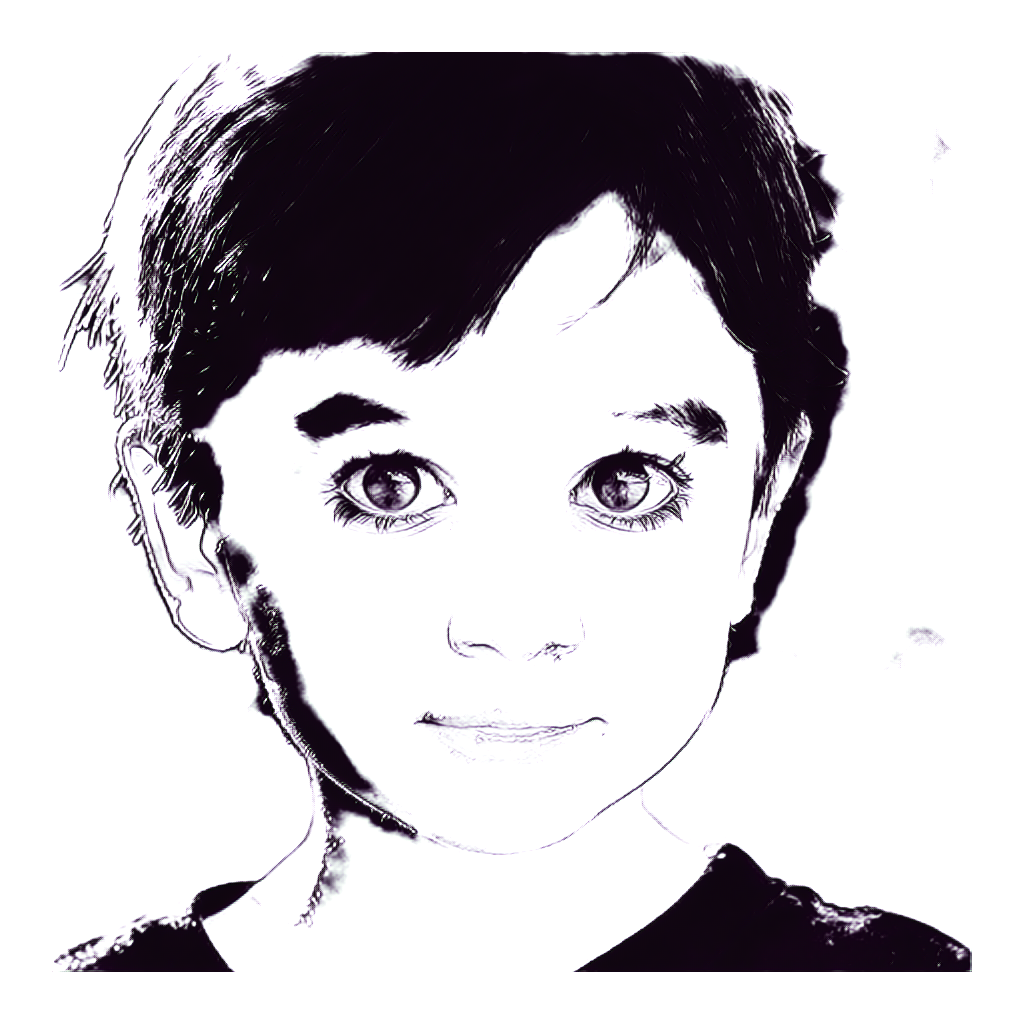
\includegraphics[width=.2\textwidth]{figures/66006-Artline.png}}
    \caption{Example of outputs obtained by using Artline}
    \label{fig:artlineRes}
\end{figure}
\noindent The performance of the four different models was evaluated and compared. The results of these models can be visualised in fig. \ref{fig:simplifyModelsRes}. The aim of this evaluation was to determine which model provided the best results for the desired application. After thorough testing, it was discovered that the MSE+GAN model and the model pencil1 both offered remarkable results, even if in different scenarios. The Artline network, as already specified, had the tendency to produce images with a high number of dark pixels, particularly in areas such as hair, facial hair and sometimes even in the background. To address this issue, the model to be used was selected based on the number of dark pixels present in the image. When the image had less than 800,000 dark pixels, the MSE+GAN model was utilised. On the other hand, for images with more dark pixels, the model pencil1 was applied.
\begin{figure}[htbp]
    \centering
    \subfloat[][\emph{MSE model}]
    {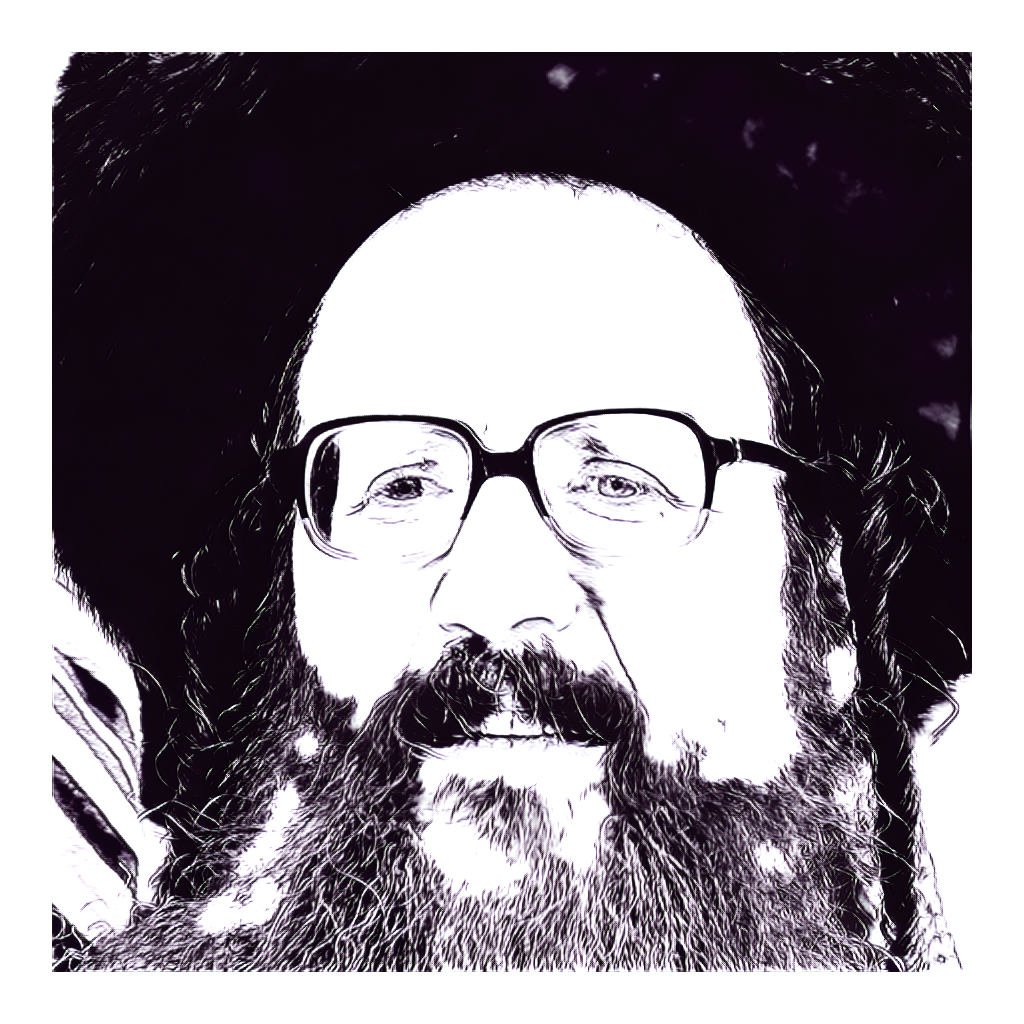
\includegraphics[width=.22\textwidth]{figures/66000Artile.png}} \quad
    \subfloat[][\emph{MSE + GAN model}]
    {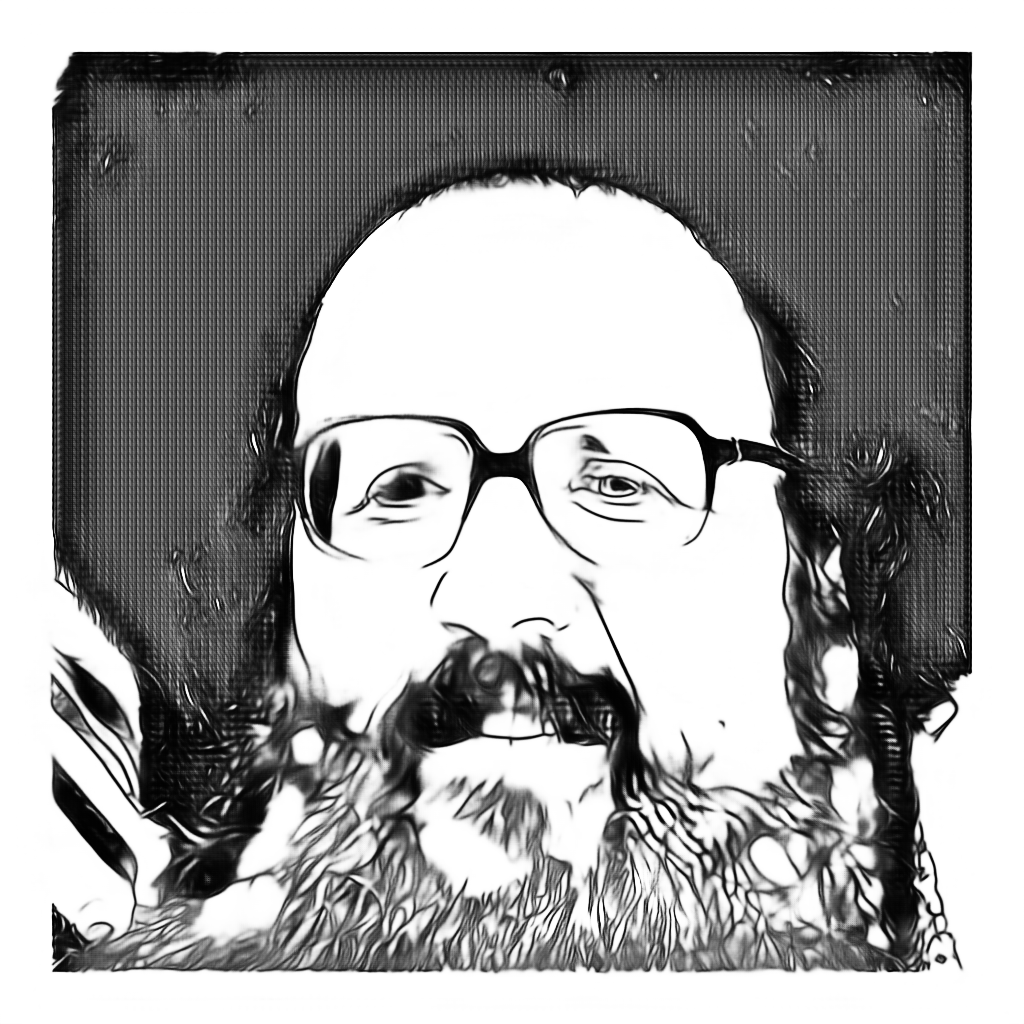
\includegraphics[width=.22\textwidth]{figures/66000mse.png}}
    \subfloat[][\emph{pencil1 model}]
    {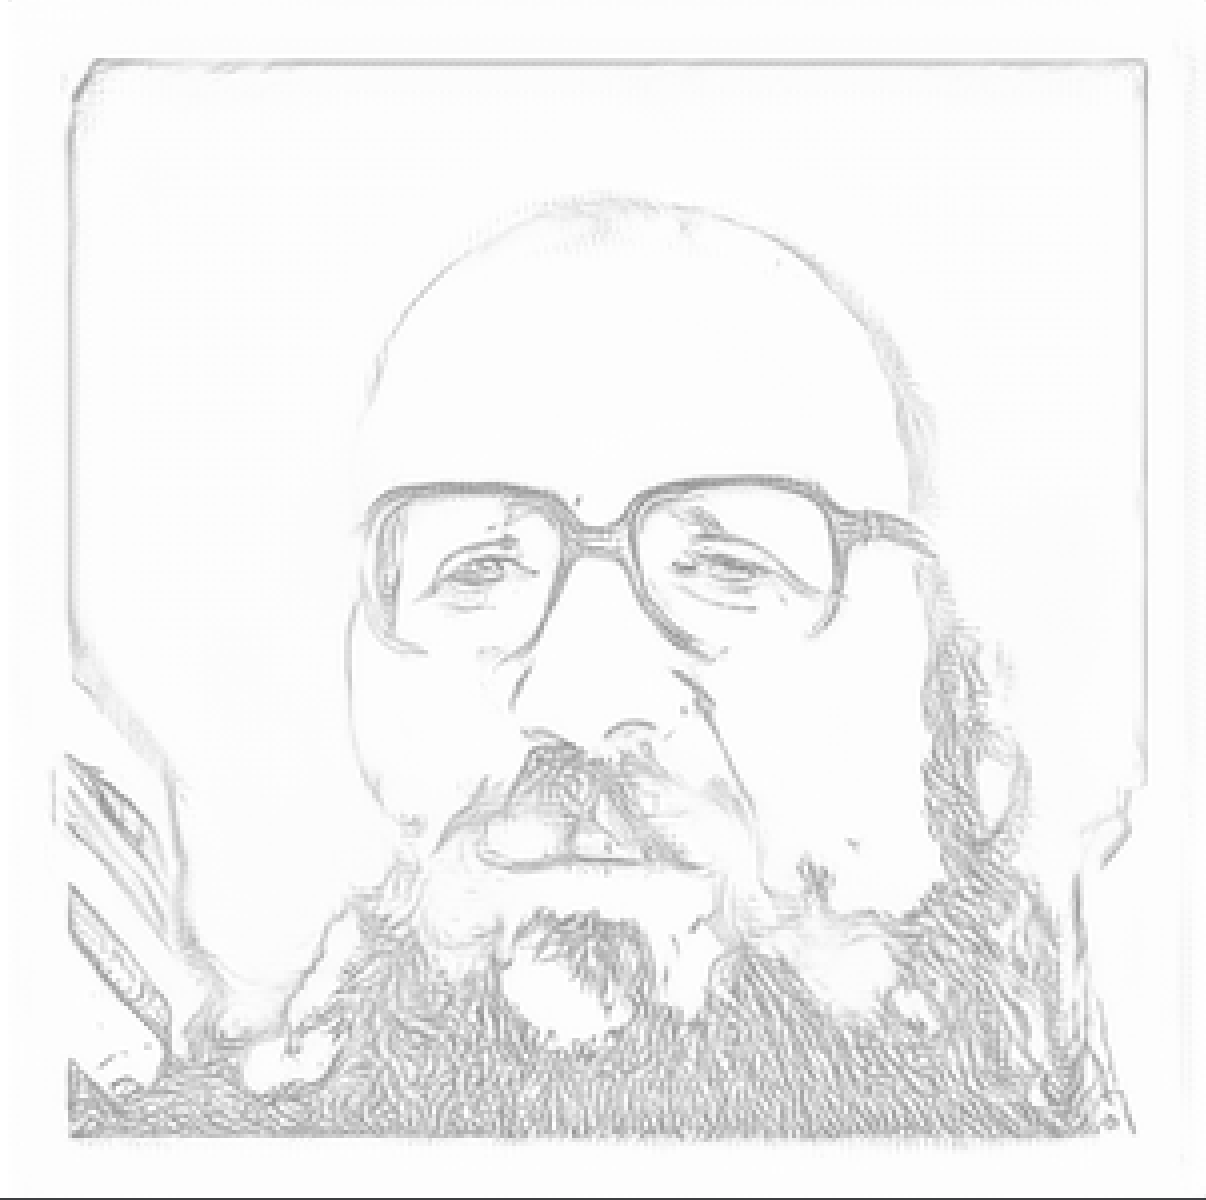
\includegraphics[width=.22\textwidth]{figures/66000-pencil1.png}}
    \subfloat[][\emph{pencil2 model}]
    {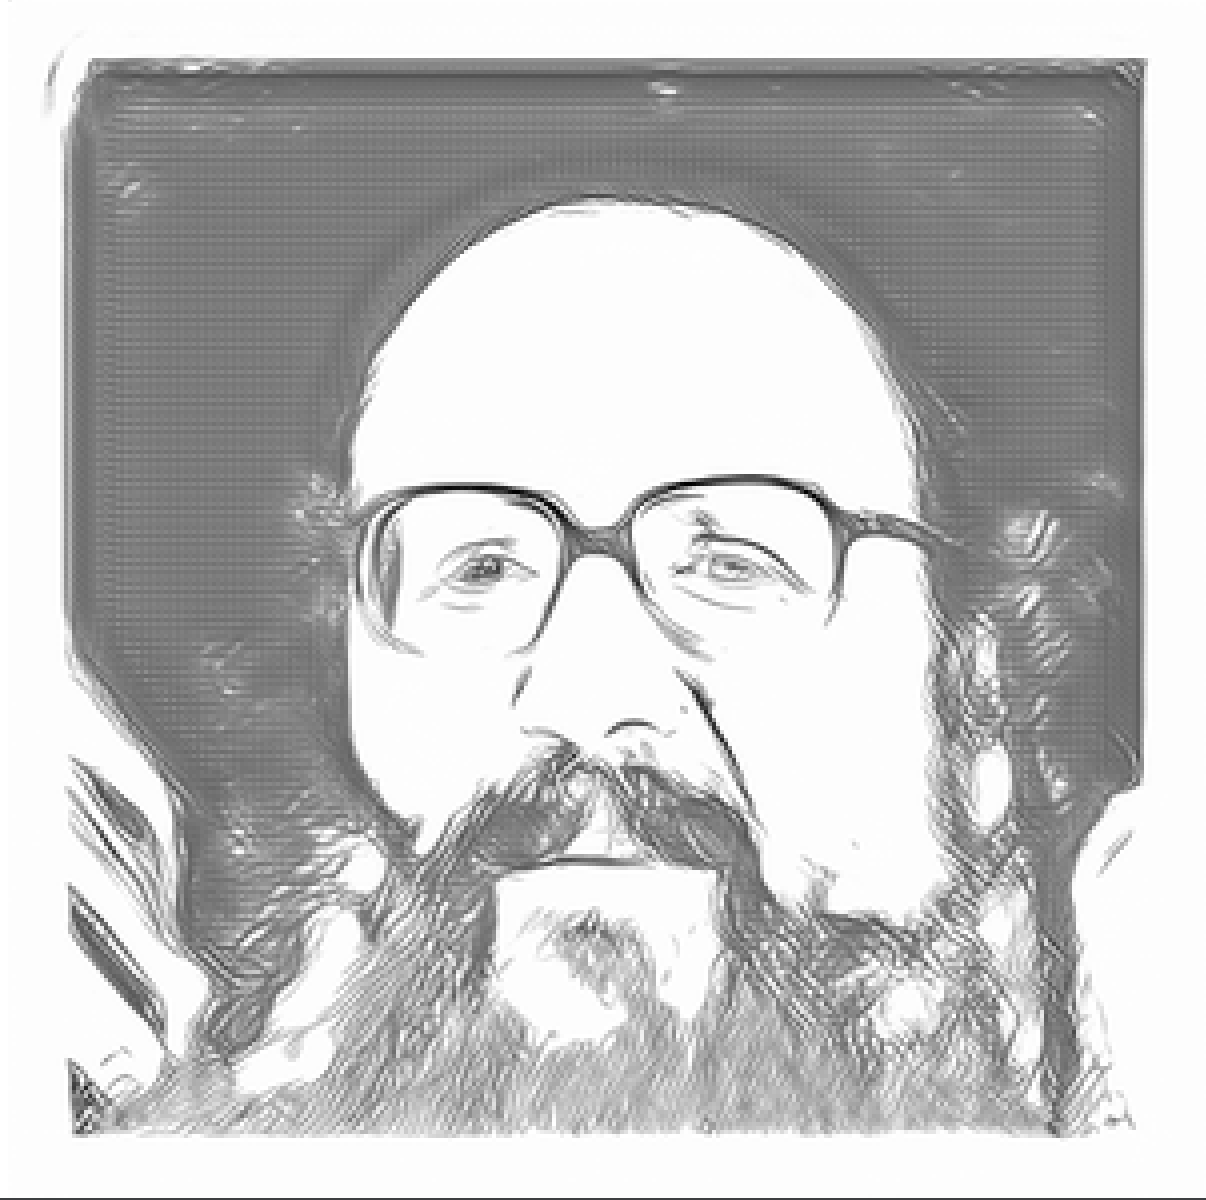
\includegraphics[width=.22\textwidth]{figures/66000-pencil2.png}}\\
    \subfloat[][\emph{MSE model}]
    {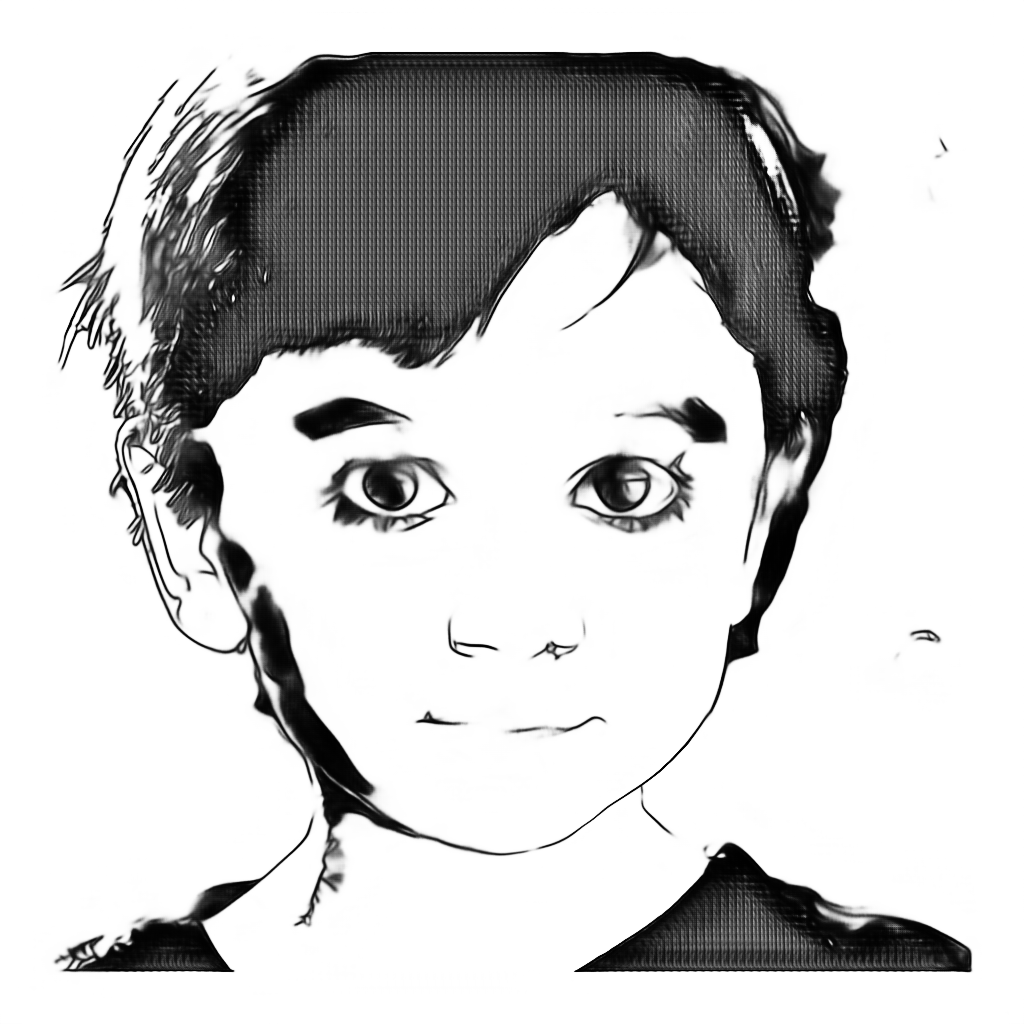
\includegraphics[width=.22\textwidth]{figures/66006-mse.png}} \quad
    \subfloat[][\emph{MSE + GAN model}]
    {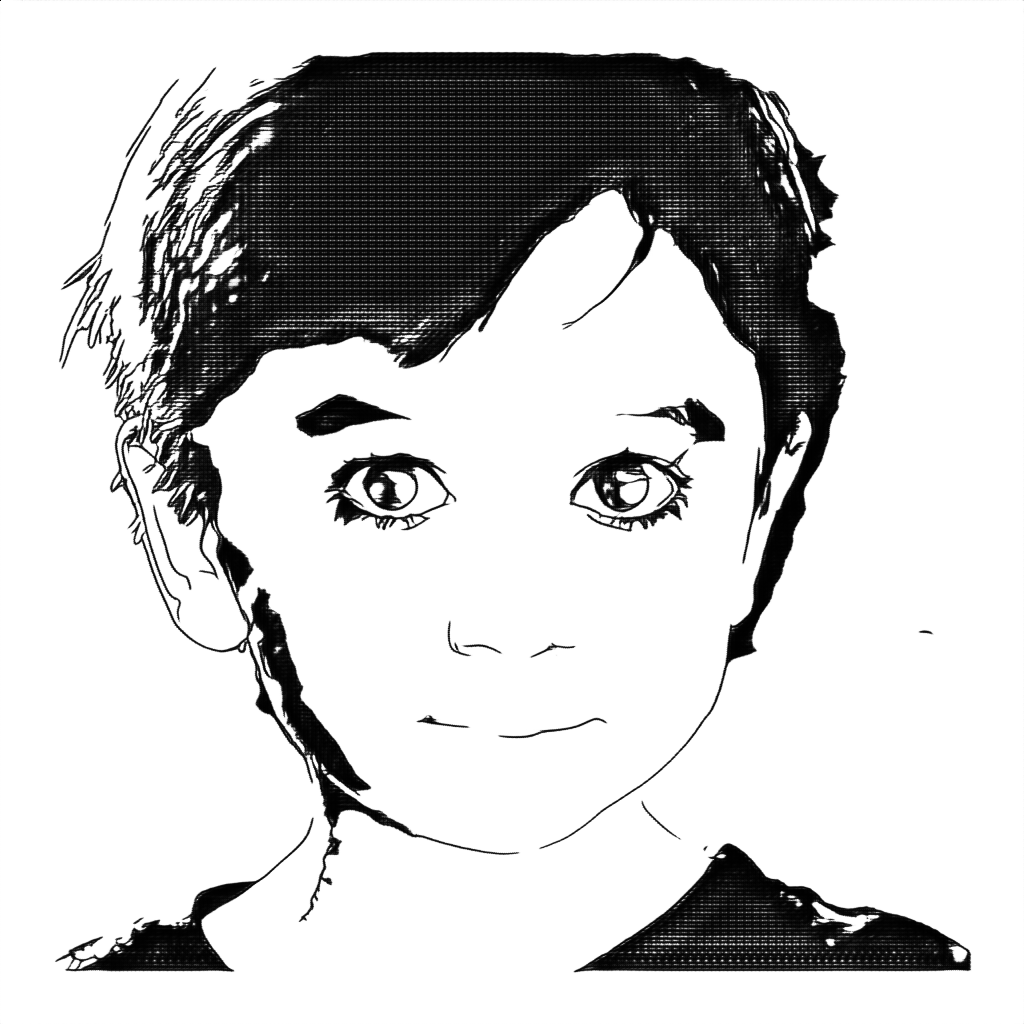
\includegraphics[width=.22\textwidth]{figures/66006-gan.png}}
    \subfloat[][\emph{pencil1 model}]
    {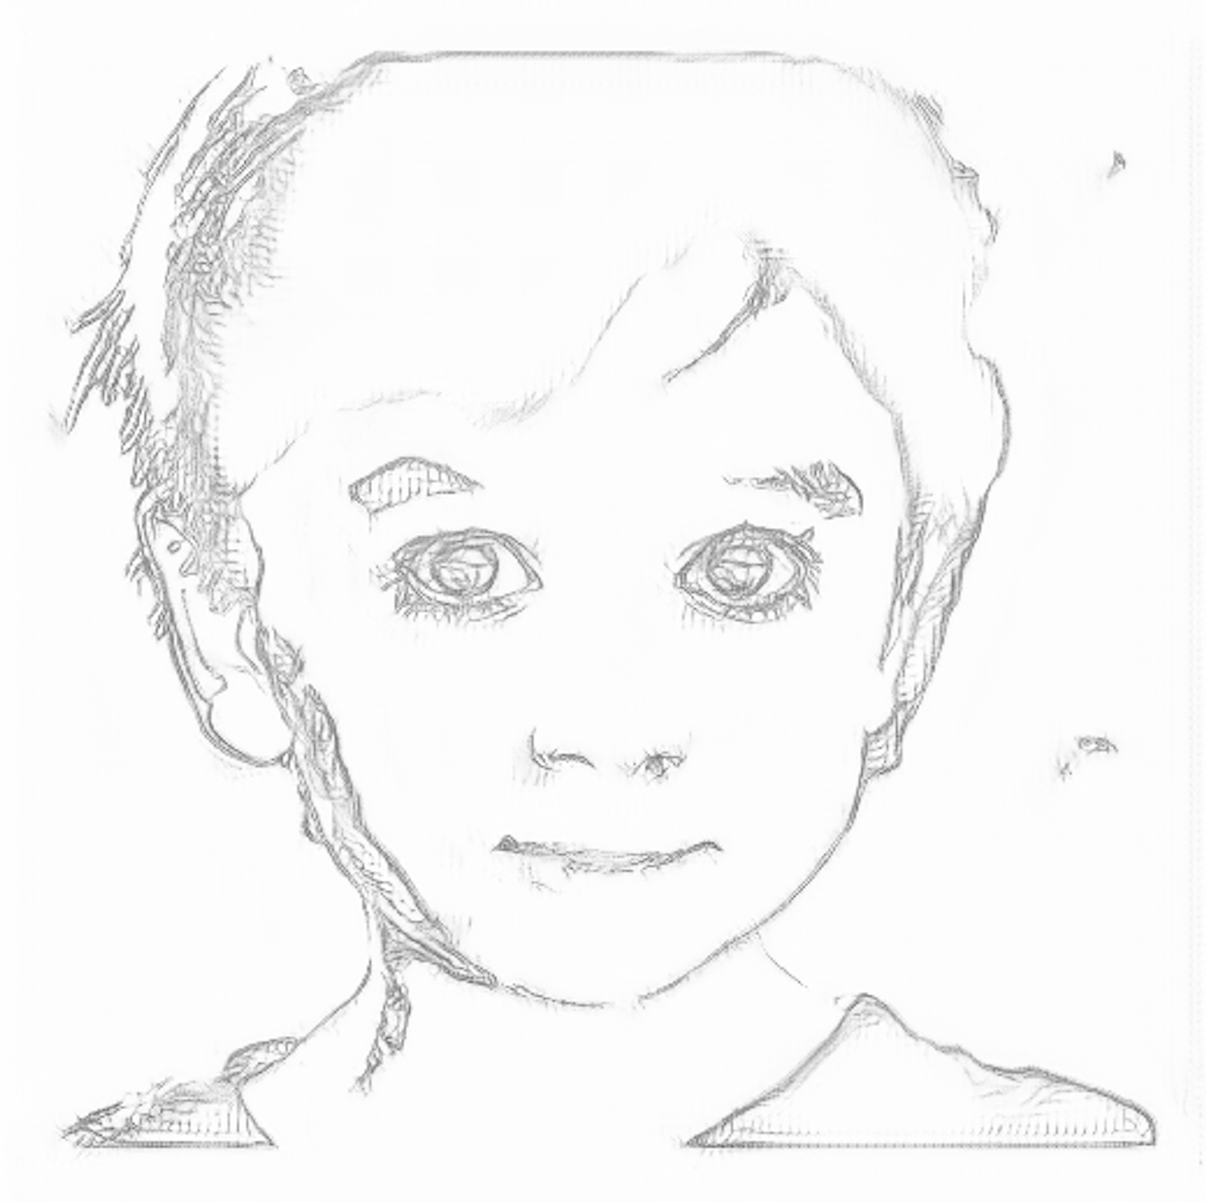
\includegraphics[width=.22\textwidth]{figures/66006-pencil1.png}}
    \subfloat[][\emph{pencil2 model}]
    {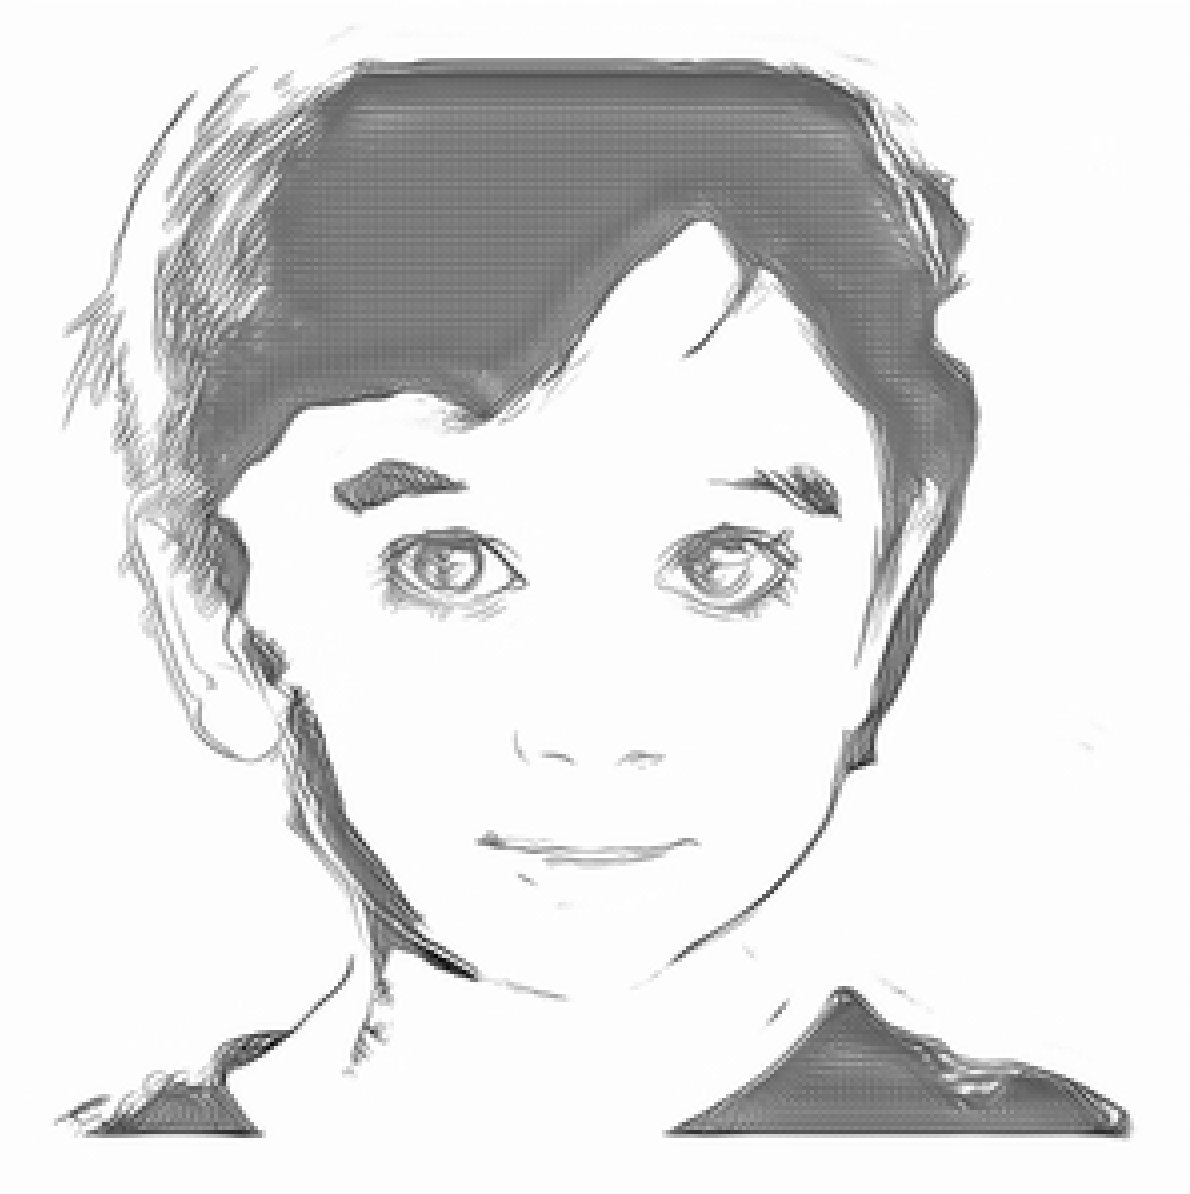
\includegraphics[width=.22\textwidth]{figures/66006-pencil2.png}}
    \caption{Output image obtained applying Artline and one of the four models of Learning to Simplify}
    \label{fig:simplifyModelsRes}
\end{figure}

\noindent After undergoing these two steps, the dataset obtained was lacking in quality as several sketches had lost some key facial features, such as lines of the lips or wrinkles. Applying the Learning to Simplify method to simplify the results from the Artline network was not the optimal solution, as Learning to Simplify is designed to convert rough sketches into clean, simplified drawings. The outcome of the network training phase responsible for generating a photo of a face from a sketch was disappointing, despite the network being trained for several days. This was due to the low quality of the dataset, which resulted in an insufficient number of high-quality sketches. To overcome this disappointment, further improvements to the dataset were required to ensure that it captured the necessary features for producing accurate facial sketches.

\noindent The new approach considered was a two-step procedure, starting with the application of an edge detection operator and then simplifying the results. While there are many available edge detection algorithms, they each have their own strengths and weaknesses. However, not all of them were suitable for this particular task, as the goal was not only to extract edges but also to produce results that resemble an artist’s sketch. Hence, the edge detector operator chosen is the XDoG operator. The results obtained with this operator are much more like drawings made by artists and are far better the one obtained using Artline. In fig. \ref{fig:xdogRes} can be seen the results of the operator used with these parameters:
\begin{itemize}
    \item $\epsilon = 0.01$
    \item $k = 200$
    \item $\sigma_1 = 0.05$,  $\sigma_2=k * \sigma_1 = 10$
    \item $\phi = 10$
\end{itemize}

\begin{figure}[htbp]
    \centering
    \subfloat[][\emph{}]
    {
\includegraphics[width=.25\textwidth]{figures/66000-xdog.png}} \quad
    \subfloat[][\emph{}]
    {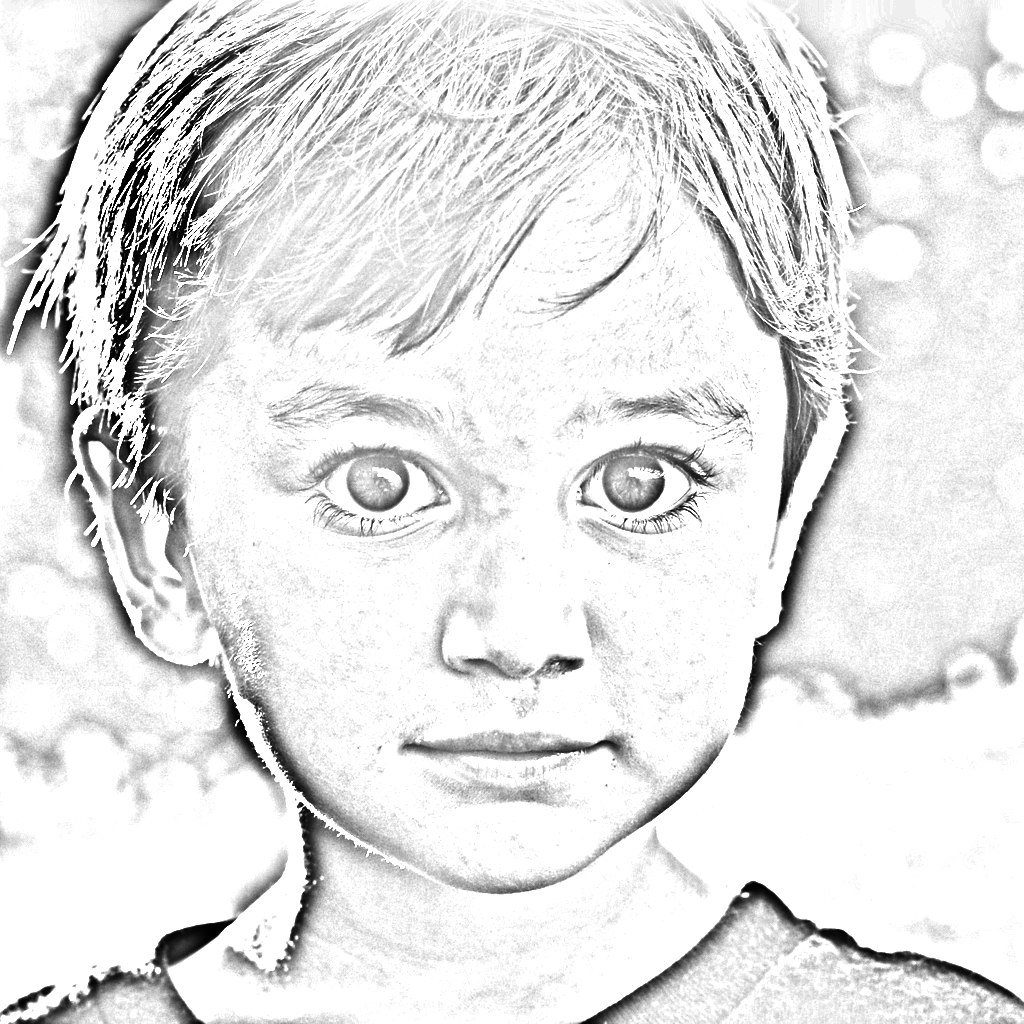
\includegraphics[width=.25\textwidth]{figures/66006-xdog.png}}
    \caption{Output image obtained applying the XDoG operator}
    \label{fig:xdogRes}
\end{figure}

\noindent Even if the results were very good, Learning to Simplify was applied in order to simplify the “sketches”. The results had to be simplified as well because the final goal is to obtain a photo of a face even if a person with no drawing ability does a sketch.
The result of this further step can be seen in fig. \ref{fig:xdogSimplifyRes}, they are significantly better compared to the ones obtained from the first approach, and it can be seen that there are preserved a lot of details that were lost in the first approach. 

\begin{figure}[htbp]
    \centering
    \subfloat[][\emph{}]
    {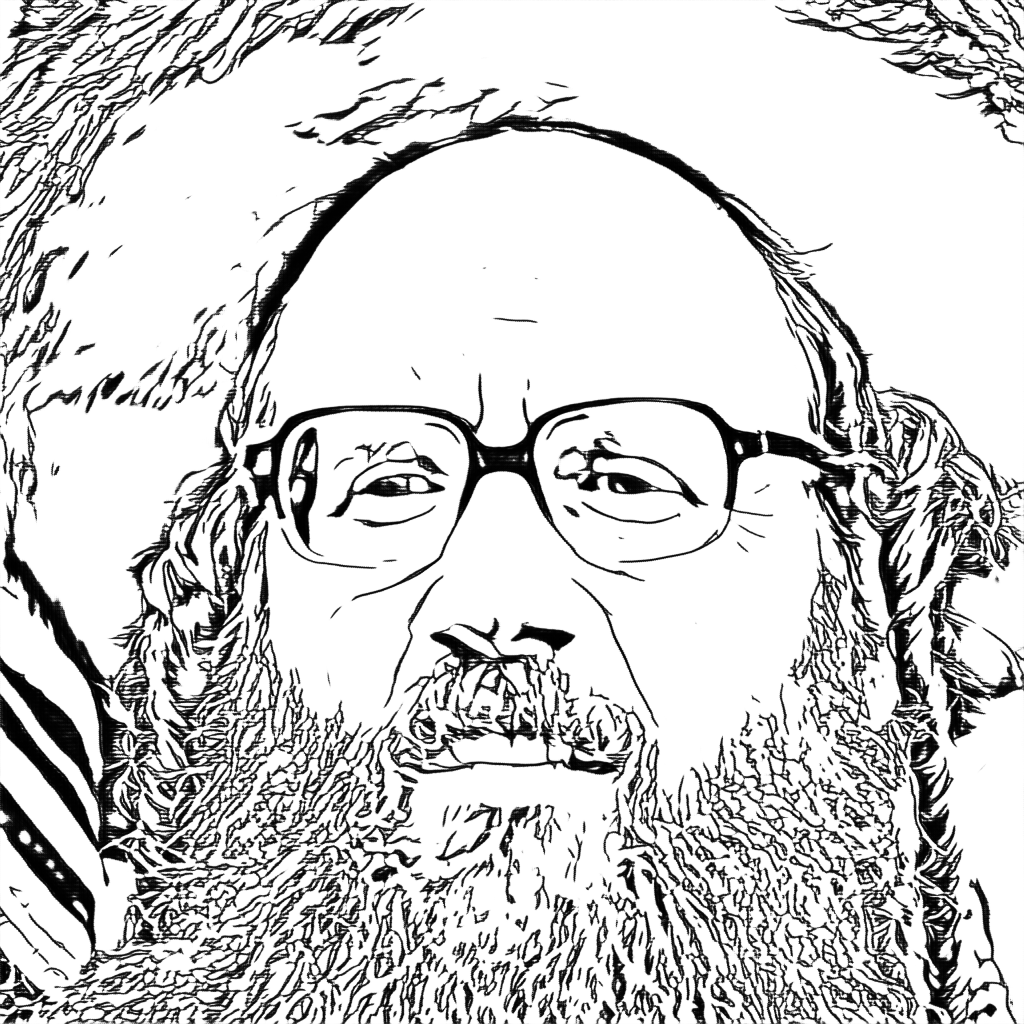
\includegraphics[width=.25\textwidth]{figures/66000-xdog-simplify.png}} \quad
    \subfloat[][\emph{}]
    {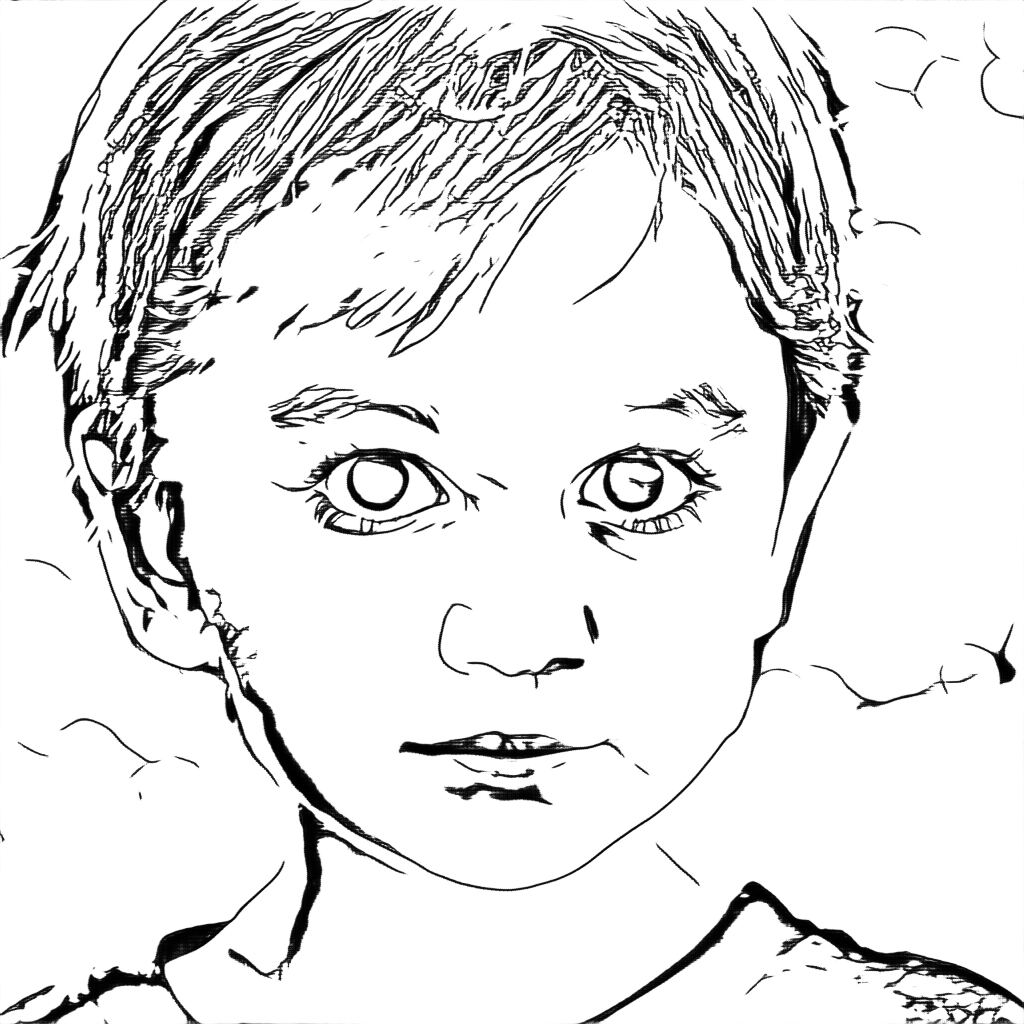
\includegraphics[width=.25\textwidth]{figures/66006-xdog-simplify.png}}
    \caption{Output image obtained applying Learning to Simplify to the output image of XDoG operator}
    \label{fig:xdogSimplifyRes}
\end{figure} % CAP 3
\newpage
\section{Implementation}
\label{sec:used GAN discussion}
% dire che adesso andrò a descrivere le reti che ho usato per ottenre una rete in grado di generare immagini quando condizioanta a uno sketch. 
In this chapter, the generative adversarial networks used to generate synthetic images starting from a sketch are described. 
% *******************************************
%\subsection{GAN configuration}
\subsection{StyleGAN}
\label{section:StyleGAN}
StyleGAN~\cite{StyleGAN} is a state-of-the-art deep learning generative model developed by NVIDIA in 2018 to produce realistic-looking images. The model is based on Generative Adversarial Network (GAN) architecture, in particular, it is built upon the foundation of the ProGAN~(\ref{sec:proGAN}), and it takes inspiration from the concept of “style transfer” introduced by~\cite{ImageStyleTransfer} to generate unique images. An approach that involves the use of neural representations to separate and recombine the content and style of images.

\noindent StyleGAN is designed to generate high-resolution images of faces, but can also be adapted to generate other types of images as well. Its key feature includes the ability to generate high-resolution images while also controlling various aspects of the image style, such as colour, texture, and overall composition. \\

\noindent The main idea behind StyleGAN is to use a deep neural network that is trained to generate images from a random noise input. This noise input is then transformed into a feature representation, which is fed into a generator network. The generator network uses a series of convolutional layers to upsample the feature representation and generate the final image. 
The generator in StyleGAN begins by using a learned constant input and then modifies the style of the image in every convolution layer based on the latent code. This direct control allows for the adjustment of the strength of the image's features at various scales. 
The inclusion of noise directly injected into the network results in the automatic, unsupervised separation of high-level attributes such as pose and identity from stochastic variations like freckles and hair in the generated images. This design makes it possible to perform intuitive mixing and interpolation operations that are specific to different scales.

\noindent The design of StyleGAN is different from the one of the traditional GANs, since the latent code is not provided to the generator through an input layer. However, the generator starts by using a $4\times4\times512$ constant to start the image synthesis process, and uses a non-linear mapping network to map the input latent code $z$ to an intermediate space. 
The non-linear mapping function is a function $f:Z\rightarrow W$ where $Z$ is the input latent space and $W$ is the intermediate latent space. This mapping network outputs a vector that controls the style of the generated image by integrating it into the generator model through the adaptive instance normalisation layer. This vector provides the ability to dictate the style of the synthetic image.
For simplicity, the authors set the dimensionality of both the input latent space and the intermediate latent space to \num{512} and the mapping is done using a \num{8}-layer Multi-Layer Perceptron (MLP). This choice of dimensionality is arbitrary and could potentially be changed in other implementations.

\noindent The purpose of the mapping network is to convert an input vector into an intermediate vector that governs different visual attributes. This is a challenging conversion since the input vector must adhere to the probability density of the training data, therefore it conducts to an entanglement of features. To solve this issue, the mapping network is used to create an intermediate vector that does not have to follow the distribution of the training data, allowing for a disentangled representation. Disentanglement representation refers to the ability of a machine learning model to identify and separate the underlying factors of variation in a set of data. This means that the model is able to identify and isolate the different aspects of the data that contribute to its overall appearance, such as colour, shape, texture, and lighting, among others.

\noindent Given the inapplicability of previous methods for determining disentanglement in the latent space in this case, the authors introduced two new automated metrics: perceptual path length and linear separability. These metrics enable them to quantify the disentanglement of the generator. Perceptual path length measures the smoothness of the generated images in the latent space. 
It is based on the idea that a small step in the latent space should correspond to a small change in the generated image. Therefore, models with low perceptual path length are expected to have a more continuous and smooth latent space. Linear separability, on the other hand, measures the degree to which different factors of variation are disentangled and can be independently manipulated in the latent space. A model with high linear separability is expected to have a latent space in which each dimension corresponds to a specific factor of variation, such as pose, identity, or background. This means that each dimension can be manipulated independently to generate new images with a specific combination of features.

%
\noindent Their results show that compared to a conventional generator architecture, their generator allows for a more linear and less entangled representation of various factors of variation.

\noindent The output of the mapping network is $512 \times 1$, the same size as the input layer. The StyleGAN generator model is now referred to as the “synthesis network” due to the integration of the new mapping network into its architecture, its architecture can be seen in Fig.~\ref{fig:StyleGAN architecture}(b), while Fig.~\ref{fig:StyleGAN architecture}(a) shows a traditional GAN architecture.
\begin{figure}[!ht]
\centering
  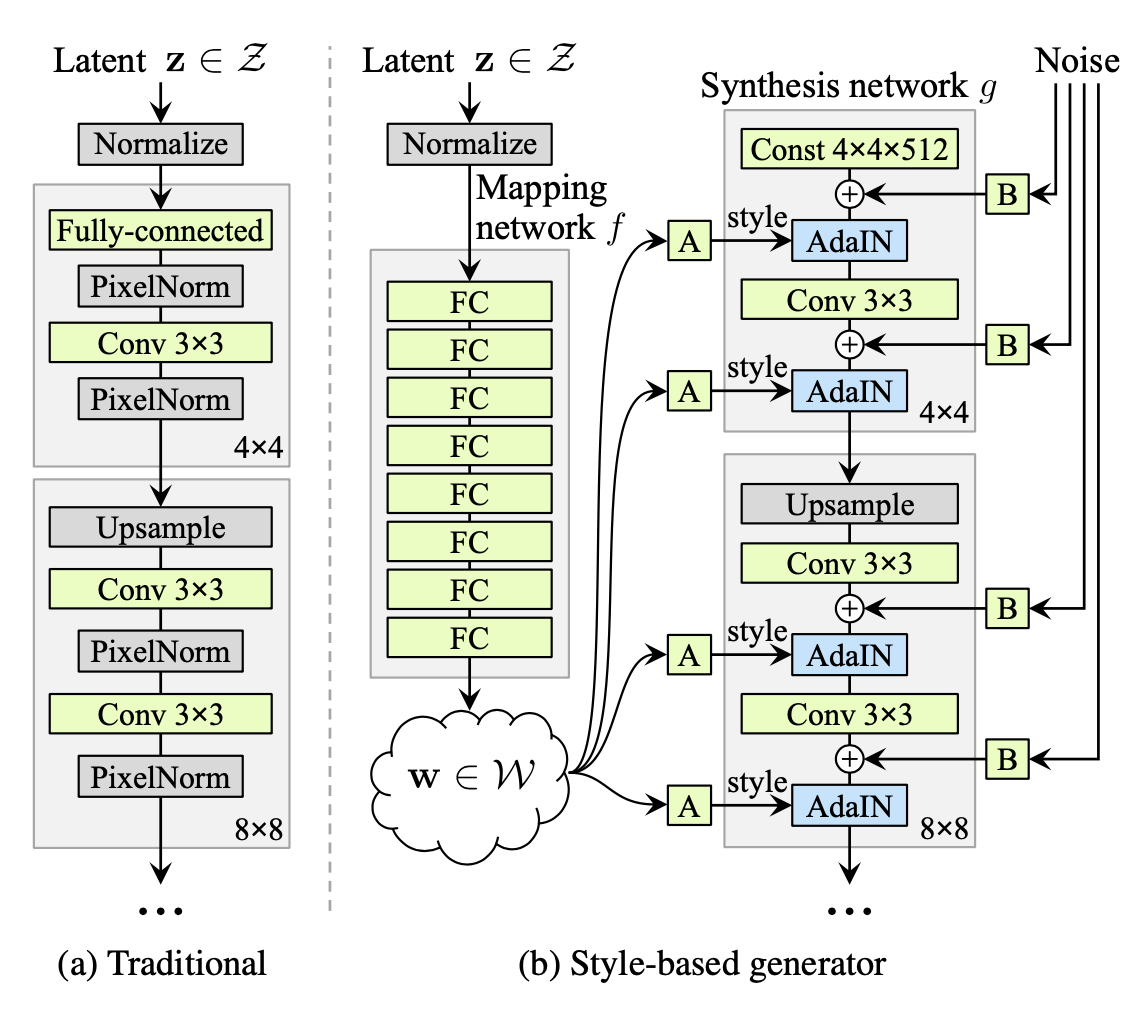
\includegraphics[scale=0.5]{figures/styleGAN-generator.png}
  \caption{(a) traditional GAN architecture, (b) Style GAN architecture. Image taken from~\cite{StyleGAN}. The mapping network consists of \num{8} layers, while the synthesis network g consists of 18 layers (two for each resolution starting from $4^2$). The “A” block stands for the affine transform, and the “B” is the block that applies per-channel scaling factor to the input Gaussian noise.}
  \label{fig:StyleGAN architecture}
\end{figure}
\\
%
\noindent The AdaIN (Adaptive Instance Normalization) layer~\cite{ArbitraryStyleTransfer} is an extension of the Instance Normalization layer which can adapt to different styles instead of being able to normalise to a single, specified style. 
The AdaIN layer integrates information from a learned encoding of the style of the image into the generator network to allow for control over the style of the generated image. This layer is added at each resolution level of the synthesis network to provide a unique visual expression of features at each level.
The AdaIN modules shift and scale the output through the layers in the synthesis network, promoting the significance of relevant filters in each convolutional layer. 
This helps the generator differentiate between important and insignificant features. It can be considered as an internal feedback mechanism, where the mapping network learns to encode the $W$ vector by focusing on the most relevant features. 
The AdaIN operation starts by normalising each channel to have zero mean and unit variance, and then it provides style information to apply scales and biases to each channel. 
The scale and bias values adjust the relative importance of each feature in the subsequent convolution operation. However, the original statistics of the input are not taken into account because of the normalisation step. As a result, each AdaIN operation only controls one convolution before being overridden by the next AdaIN operation.
The AdaIN operation receives a feature map $x_i$ and a style input $y=(y_s,y_b)$, and it is defined as:
\begin{equation}
    \mbox{AdaIN}(x_i,y)=y_{s,i}\frac{x_i - \mu (x_i)}{\sigma(x_i)}+y_{b,i}
\end{equation}

\noindent where $\mu(x_i)$ is the mean, $\sigma(x_i)$ is the variance, while for scaling and shifting $y_{s,i}$ and $y_{b,i}$ are used respectively. Since $y$ consists in a scaling and shifting factors, its dimensionality is twice the number of feature maps on that layer.
This process helps to preserve the content information from the content input while allowing the style information from the style input to be applied to the output.
Additionally, each layer of the synthesis network is fed with uncorrelated Gaussian noise before the AdaIN operation in order to generate stochastic details. Incorporating random noise at each style block enables more precise control over the model's generated details, including finer features like freckles, beard, wrinkles, and dimples. Without this noise, these small details would be overpowered by larger, more prominent features. It is evident that the noise only impacts the stochastic elements, preserving the overall composition and high-level features such as identity.\\

\noindent Moreover, the mixing regularisation technique is used to promote even more the localisation of styles in the generator. During training, a portion of the images is generated using two random latent codes instead of just one. This process, called “style mixing”, involves switching from one latent code to another at a randomly chosen point in the synthesis network. The mapping network processes the latent codes, $z_1$ and $z_2$, producing the corresponding styles $w_1$ and $w_2$, which respectively control the styles applied before and after the crossover point. This regularisation method prevents the network from assuming a correlation between adjacent styles. 

%
\noindent The authors of StyleGAN used the WGAN-GP loss function (\ref{sec:wgan}) for evaluating their method.

%%%%%%%%%%%%%%% -.----------------
\noindent The experiment conducted by Karras et al.~\cite{StyleGAN} shows that the redesign of the generator not only preserves image quality, but also it significantly enhances it. To demonstrate this, the Fréchet Inception Distance (FID) was computed for various generator architectures on a few available datasets.
The authors' results suggest that a style-based design is superior to the conventional GAN generator architecture in all aspects.
This superiority is demonstrated through established quality metrics, and their findings on the separation of high-level features and stochastic effects, as well as the linearity of the intermediate latent space, all point towards a deeper understanding and control of GAN synthesis.
Furthermore, their path length metric can be included as a regularisation term during training, and a similar approach could be applied to the linear separability metric.

\subsection{StyleGAN2}
\label{section:StyleGAN2}
StyleGAN2 (2020) is an improvement of~(\ref{section:StyleGAN}) for synthesising high-resolution images developed by NVIDIA. This new version is based on the previous one, but with some differences~\cite{Karras2019stylegan2}.
The authors of StyleGAN2 discovered that styles were not only capable of capturing and transferring the essence of an image, but also transferring visual distortions such as water droplets or smudges.
They linked these visual distortions to the AdaIN layers, and therefore they made some changes to them in order to eliminate the artefacts. 
To overcome this issue, they came up with a new approach to the AdaIN layers, which were previously used as direct inputs to the network. Instead, they integrated the AdaIN layers within the convolutional layers.

\noindent The authors replaced the AdaIN operator with a weight modulation and demodulation step, where the modulation adjusts each feature map of the convolution based on the style. 

\noindent The authors discovered that the strong location preference for facial features in StyleGAN images was due to progressive growing. To address this, they took inspiration from the “Multi-Scale Gradients for Generative Adversarial Networks” paper by Animesh Karnewar and Oliver Wang~\cite{karnewar2019msg} and incorporated the idea of multiple scale gradient using a single architecture. They developed a new architecture, which can be seen in Fig.~\ref{fig:StyleGAN2 architecture}, that employs multiple scales of image generation, which is achieved through the utilisation of a resnet-style skip connection that links lower resolution feature maps to the final generated image.
 \begin{figure}[htbp]
\centering
  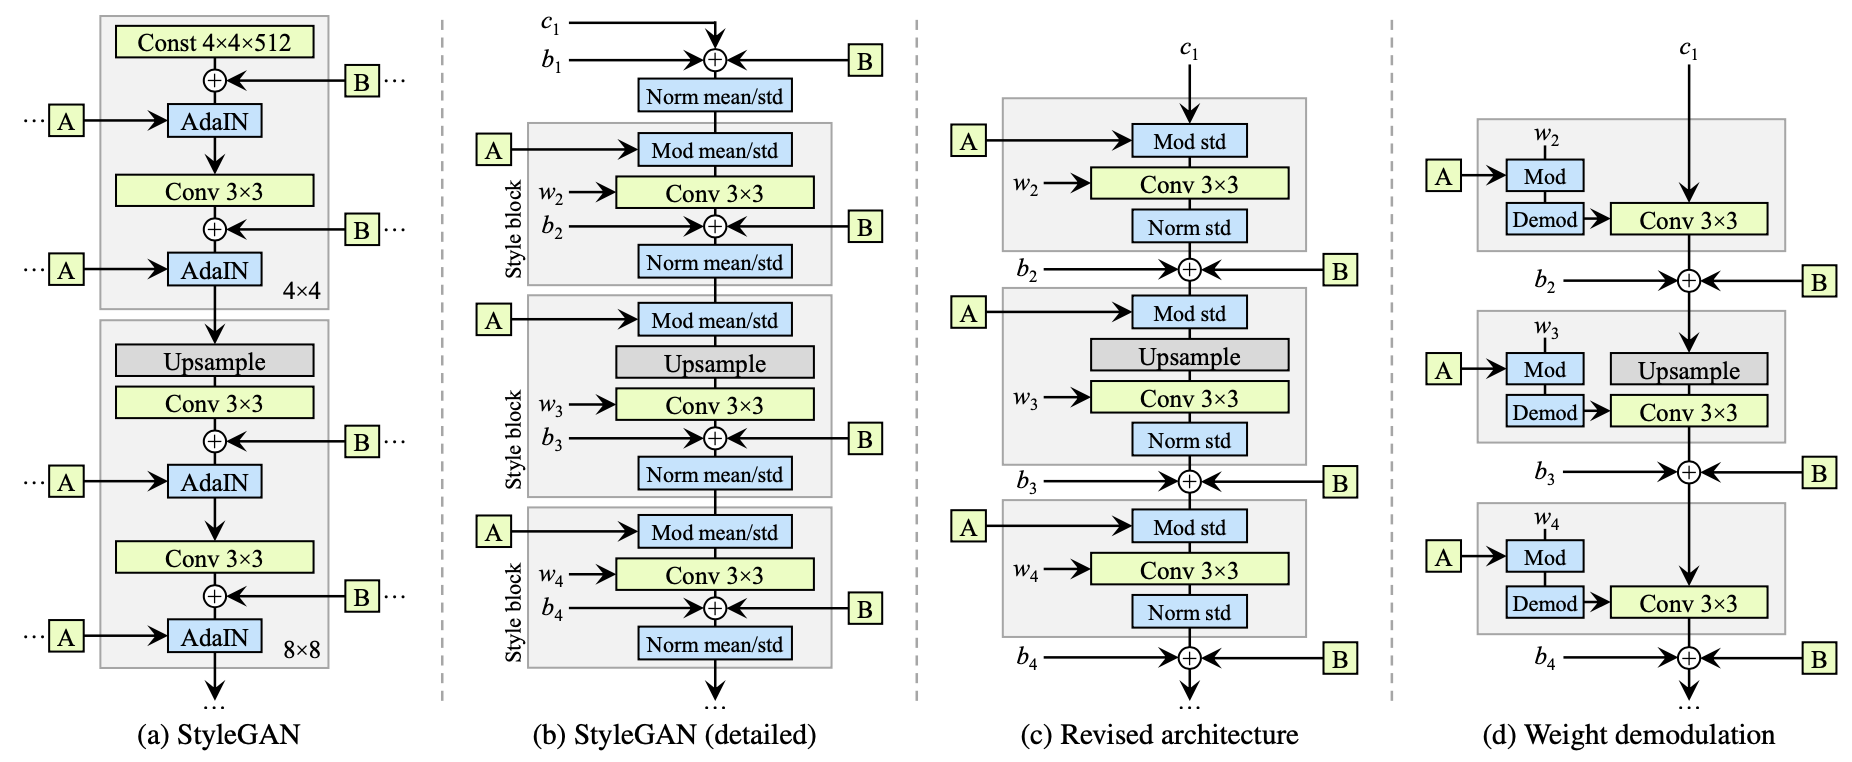
\includegraphics[scale=0.4]{figures/StyleGAN2-architecture.png}
  \caption{StyleGAN2 architecture. Image taken from \cite{Karras2019stylegan2}. Fig (a) and (b) show the StyleGAN architecture and its detailed view. In fig (c), the StyleGAN architecture in which the AdaIN layers have been replaced with the modulation is illustrated. Fig. (d) shows the revised architecture in which the instance normalisation has been replaced with a “demodulation” operation.}
  \label{fig:StyleGAN2 architecture}
\end{figure}

\noindent A further difference between the two version of StyleGAN is the introduction of a normalisation term to the loss function to make the latent space more uniform and smoother. By doing so, the mapping of images in and out of the latent space becomes more controlled, enabling more controlled image generation. Additionally, this improved relationship between the latent space and generated images allows creating images along a path in the latent space. The regularisation term added to the loss is driven by the goal of maintaining the expected lengths of vectors regardless of their directions, and it is formulated as:
\begin{equation}
    \mathbb{E}_{\mathbf{w,y}\sim \mathcal{N}(0,1)}=(\| \mathbf{J_w}^T\mathbf{y}\|_2 - a)^2
\end{equation}
where $\mathbf{y}$ are random images with normally distributed pixel intensities, $\mathbf{w} \sim f(\mathbf{z})$, where $\mathbf{z}$ are normally distributed. The local metric properties of the generator's mapping function $g(\mathbf{w}): \mathcal{W}\rightarrow \mathcal{Y}$ are represented by the Jacobian matrix $\mathbf{J_w}=\partial g(\mathbf{w})/\partial \mathbf{w}$.
The value of the constant $a$ is dynamically determined during the optimisation process through the calculation of the long-term exponential moving average of the vector lengths $\| \mathbf{J_w}^T\mathbf{y} \|_2$. This allows the optimisation to automatically find an appropriate global scale for the process.

\noindent The regularisation term is known as \textit{path length regularisation}, and its implementation has proven to be highly beneficial in practice, leading to the development of more stable and consistent models. This makes the process of exploring and experimenting with different architectural designs much more manageable. Additionally, it has been noted that the smoother nature of the generator as a result of this regularisation makes it significantly easier to perform inversion.\\ 

%%%
\noindent Additionally, the authors~\cite{Karras2019stylegan2} observed that there was no need to compute the regularisation term every time the loss was computed, therefore in this way they could obtain a decrease in the computational cost and also in the overall memory usage. They applied a lazy regularisation and evaluate the regularisation terms every $k$ training iterations.

\noindent To summarise the improvements made in the second version of StyleGAN are:
%which leads to the removal of artifacts in generated images, enforcement of smoother latent space interpolation and reduction of the strong location preference for facial image features, are:
\begin{enumerate}
\setlength{\itemsep}{1pt}
\setlength{\parskip}{0pt}
\setlength{\parsep}{0pt}
    \item weight demodulation
    \item path length regularisation
    \item lazy regularisation
    \item no growing
\end{enumerate}
These improvements made it also possible to speed up the learning time of the model up to \num{40}\% and optimise the images quality.

% this integration allowed for parallel computation, significantly boosting the speed of training the model by up to \num{40}\% and reducing the appearance of visual distortions.
%%%%%%%%%%%%%%%%%%%%%%%%%%%%%%%%%%%%%%%%%%%%%%%%%%
\subsection{pSp Framework}
\label{section:pspFramework}
Pixel2Style2Pixel (pSp) is a novel image translation framework that leverages the powerful representation capabilities of a pre-trained StyleGAN2 generator and the extended $\mathcal{W}+$ latent space~\cite{pSp}. The pSp framework is designed to tackle the task of transforming an input image into a target image, preserving the content of the original image while adopting the style of another.
In the paper, a new encoder network is proposed, it is based on a Feature Pyramid Network capable of directly encoding real images into the $\mathcal{W}+$ space.

\noindent The encoder that the authors built is able to directly reconstruct real input images, enabling latent space manipulations without the need for time-consuming optimisation. However, this approach is limited as the input image must be invertible, meaning that it must have a latent code that can reconstruct it. This is a critical limitation since in conditional image generation, the input image does not stay in the same StyleGAN domain. The solution proposed is to utilise the encoder jointly with the pre-trained StyleGAN generator as a complete solution for image-to-image translation, thereby overcoming the limitation of the encoder's requirement. 

\noindent The input images are transformed into the desired output latents through direct encoding, which are then processed by StyleGAN to generate the desired output images. In this way, StyleGAN can be used for image-to-image translation also when the input and output images belong to different domains.

\noindent The straightforward way to encode an input image into the $\mathcal{W}+$ is to extend the encoder backbone with a feature pyramid which allows to produce three levels of features maps of spatial resolution (coarse, medium and fine).
%
The styles are extracted from different scales of the pyramid using an intermediate network called \textit{map2style}, and are inserted directly into the fixed, pre-trained StyleGAN2 generator in correspondence to their scale to generate the final output image.
The \textit{map2style} is a small fully convolutional network which reduces the spatial size using a set of 2-strided convolutions followed by LeakyReLU activation functions. It is trained to extract the learned style from the corresponding feature map for each of the 18 target styles. Figure~\ref{fig:pSp encoder architecture} illustrates the pSp architecture.
 \begin{figure}[htbp]
\centering
  \includegraphics[scale=0.43]{figures/psp-architecture.png}
  \caption{Pixel2Style2Pixel architecture. Image taken from \cite{pSp}}
  \label{fig:pSp encoder architecture}
\end{figure}

\noindent Additionally, they wanted to design the encoder to learn the latent code based on an average style vector in order to improve the initialisation. Therefore, they defined an average style vector $\mathbf{\Bar{w}}$ of the pretrained generator, and given an input image $\mathbf{x}$ the output of their model is defined as:
\begin{equation}
    pSp(\mathbf{x}) := G(E(\mathbf{x}) + \mathbf{\Bar{w}})
\end{equation}
where $E(\cdot)$ is their encoder while $G(\cdot)$ is the StyleGAN2 generator.

\noindent For the loss function, the authors used a weighted combination of several functions, since they observe that this combination allowed to obtain a more accurate encoding into StyleGAN, defined as: 
\begin{equation}
    \label{eq:pSpTotalLoss}
    \mathcal{L}(\mathbf{x}) = \lambda_1 \mathcal{L}_2(\mathbf{x}) + \lambda_2 \mathcal{L}_{LPIPS}(\mathbf{x}) + \lambda_3\mathcal{L}_{reg}(\mathbf{x}) + \lambda_4\mathcal{L}_{ID}(\mathbf{x})
\end{equation}
where $\lambda_1,\lambda_2,\lambda_3,\lambda_4$ are constants used to define the loss weights, and $\mathcal{L}_2$ loss is the pixel-wise loss:
\begin{equation}
    \label{eq:l2Loss}
    \mathcal{L}_2 =  \| \mathbf{x} - pSp(\mathbf{x})  \|_2
\end{equation}
 $\mathcal{L}_{LPIPS}$ is the LPIPS loss to learn perceptual similarities, with $F(\cdot)$ denoting the perceptual feature extractor:
\begin{equation}
    \label{eq:lpips-loss}
    \mathcal{L}_{LPIPS} = \| F(\mathbf{x} - pSp(\mathbf{x})) \|_2
\end{equation}
$ \mathcal{L}_{reg}$ is the regularisation loss to guide the encoder to produce latent style vectors that are closer to the average latent vector:
\begin{equation}
    \label{eq:regularizationLoss-psp}
    \mathcal{L}_{reg} = \| E(\mathbf{x}) - \mathbf{\Bar{w}}\| _2
\end{equation}
and finally $ \mathcal{L}_{ID}$ is a loss measuring the cosine similarity between the output image and its source since their aim was to preserve the input identity:
\begin{equation}
    \label{eq:identityLoss}
    \mathcal{L}_{ID}(\mathbf{x}) = 1 - \langle R(\mathbf{x}) - R(pSp(\mathbf{x}))\rangle
\end{equation}
where R represents the ArcFace pretrained network~\cite{arcface2018}, which is a type of loss function that aims to increase the separability between classes by adding a margin to the cosine similarity between features of an image and the weight vector of the classifier.
%
%
%
%%%%%%%%%%%%%%%%%%%%%%%%%%%%%%%%%%%%%%%%%%%%%%%%%%%
\subsection{Restyle}
\label{section:restyle}
In the area of unconditional image synthesis, Generative Adversarial Networks have recently achieved outstanding results. 
It is essential for trained GANs to be able to invert an image into its matching latent code, since doing so allows manipulating real-world images while exploiting the network's rich semantics.
One of these models is StyleGAN, which is capable of synthesising highly realistic images, as discussed in~\ref{section:StyleGAN}. However, there is a major drawback to StyleGAN: it only allows for the synthesis of new images in a specific style, meaning that it cannot change the style of an existing image.

\noindent This limitation has motivated the development of the ReStyle algorithm~\cite{alaluf2021restyle}, which is a residual-based StyleGAN encoder that can change the style of an existing image. The ReStyle algorithm is based on the iterative refinement of a residual encoding that transforms the input image into a feature representation compatible with the StyleGAN generator. In this way, ReStyle permits to transfer the style from a pre-trained StyleGAN2 model to a given input image.

\noindent In the paper “ReStyle: A Residual-Based StyleGAN Encoder via Iterative Refinement”~\cite{alaluf2021restyle}, the authors presented a new encoder-based inversion approach for a more accurate image inversion. They observed that achieving precise inversion in a single attempt inflicts a heavy constraint on the training process, so they introduced a novel method, called \textit{ReStyle}, that employs an iterative process to carry out the inversion. This method uses a feedback mechanism to repeatedly feed the output of each iteration back into the encoder together with the original input image. This enables the encoder to use the knowledge gained from previous iterations to focus on the important parts necessary to reconstruct the input image with a certain level of accuracy.

\noindent The objective is to train an encoder $E$ capable of inverting real-world images into the extended $\mathcal{W}+$ latent space of a previously trained StyleGAN generator $G$. Where the goal must be achieved through multiple steps $N>1$, with each step consisting of a single forward pass through both the encoder and the StyleGAN generator.

\noindent From a mathematical point of view, the purpose was to generate an image $\hat{\textbf{y}} = G(E(\textbf{x}))$, where $\textbf{x}$ is a given input image, in such a way that $\hat{\textbf{y}} \approx \textbf{x}$. To reach this goal, the encoder was trained while the StyleGAN generator remained fixed, since it is pre-trained.\\

%\subsubsection{ReStyle training}
\noindent \textbf{ReStyle training}

\noindent To train the encoder network and enable it to perform the inversion task, a set of losses are introduced. The losses used, which are also used by most encoder-based methods, are a L2 loss, which measures the difference between the reconstructed image and the original image pixel-wise, and a perceptual loss, such as LPIPS, which measures the difference between the two images in terms of their high-level features. 
The training process of the encoder is guided by the losses, which are computed at each forward step. The encoder weights are then updated according to the computed losses via back-propagation. In the inversion process at step $t$, ReStyle operates by concatenating the current prediction of the reconstructed image $\hat{\textbf{y}}$ with an input image $\textbf{x}$. This results in an extended \num{6}-channel input, represented as $\textbf{x}_t$:
\begin{equation}
\label{eq:concatenationXandCurrentPred}
    \textbf{x}_t := \textbf{x} \| \hat{\textbf{y}}_t
\end{equation}
At this point the encoder E has to compute the residual code based on the latent code just predicted, and then it updates the new prediction for the latent code using the previous latent code $w_t$, as shown in equations~\ref{eq:residualComputation} and~\ref{eq:latentCodeUpdate}, respectively.
%update the latent code's prediction to the inversion of the input image, as shown in equations \ref{eq:residualComputation} and \ref{eq:latentCodeUpdate}, respectively.
\begin{equation}
    \label{eq:residualComputation}
    \Delta_t := E(\textbf{x}_t)
\end{equation}
\begin{equation}
    \label{eq:latentCodeUpdate}
    \textbf{w}_{t+1} \xleftarrow{} \Delta_t + \textbf{w}_t
\end{equation}
The updated prediction of the reconstructed image is obtained by passing the latent code $\textbf{w}_{t+1}$ to the generator, as defined in equation~\ref{eq:updatePredictionOfReconstructed}. Finally, the updated estimate $\hat{y}_{t+1}$ is used in the following step, as specified by equation~\ref{eq:concatenationXandCurrentPred}.
\begin{equation}
    \label{eq:updatePredictionOfReconstructed}
    \hat{\textbf{y}}_{t+1} := G(\textbf{w}_{t+1})
\end{equation}
The initialization of the inversion process consists in starting with an average latent code $w_0$ and its corresponding image $\hat{y}_0$, the overall process can be seen in Figure~\ref{fig:ReStyle inversion scheme}.
 \begin{figure}[htbp]
\centering
  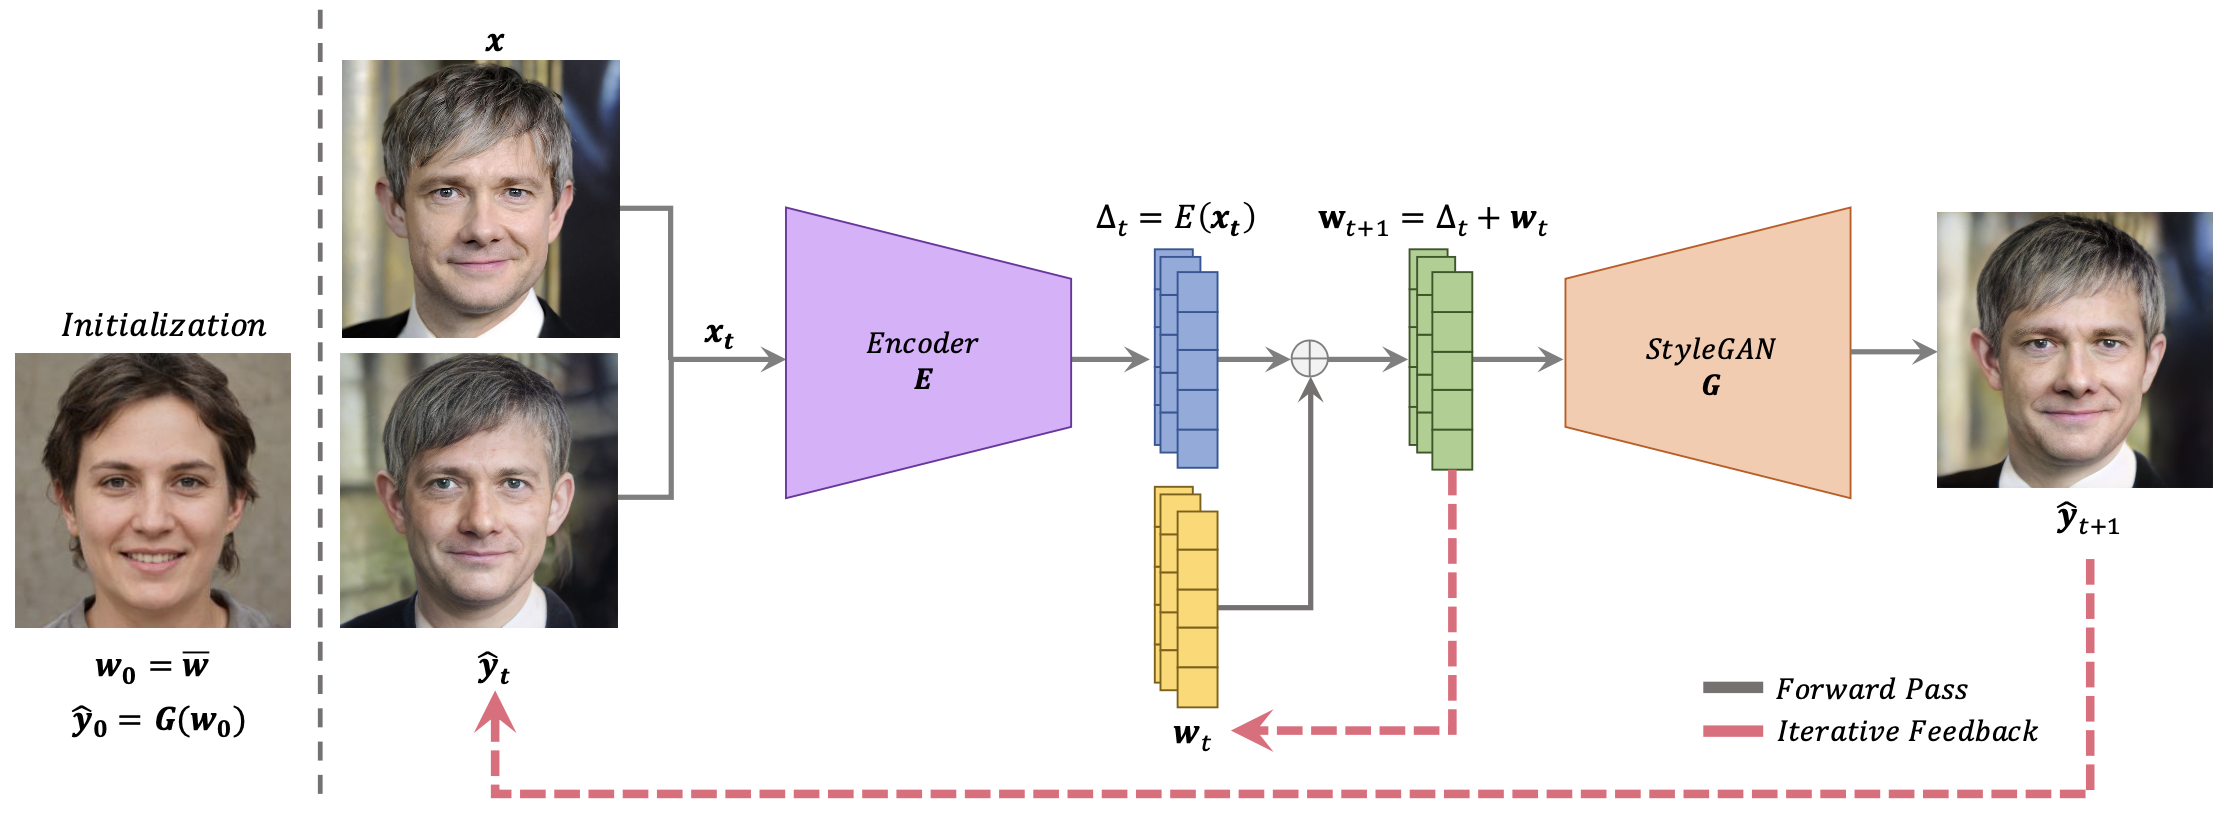
\includegraphics[scale=0.3]{figures/restyle-inversionScheme.png}
  \caption{ReStyle's iterative inversion process. Image taken from~\cite{alaluf2021restyle}}
  \label{fig:ReStyle inversion scheme}
\end{figure}

%\subsubsection{ReStyle Encoder architecture}
\noindent \textbf{ReStyle Encoder architecture}

\noindent The ReStyle encoder (Fig.~\ref{fig:ReStyle encoder architecture}) is designed as a variation of the architecture described in~\ref{section:pspFramework} and by~\cite{e4e}. Instead of obtaining the style features from three intermediate levels in the encoder, all style vectors are derived from the final 16×16 feature map. To do so, k different \textit{map2style} blocks are employed to reduce the size of the feature map and produce the corresponding \num{512}-dimensional style input, where $k$ is the number of style inputs in the StyleGAN generator, as introduced in~\ref{section:pspFramework}.\\
 \begin{figure}[htbp]
\centering
  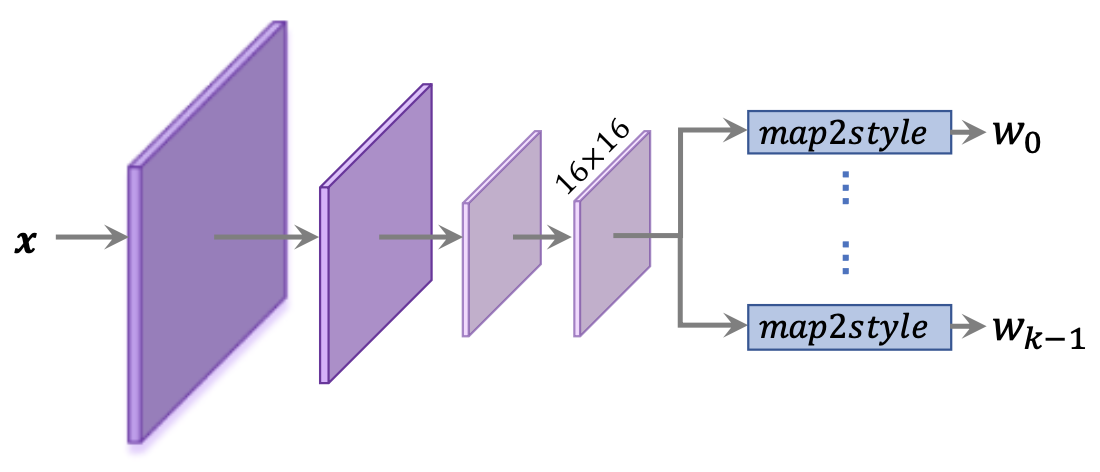
\includegraphics[scale=0.5]{figures/restyle-encoderArchitecture.png}
  \caption{Simplified ReStyle encoder architecture. Image taken from~\cite{alaluf2021restyle}}
  \label{fig:ReStyle encoder architecture}
\end{figure}


% \subsubsection{ReStyle conclusion}
\noindent \textbf{ReStyle conclusion}

\noindent The ReStyle scheme has been shown to produce highly realistic results in a variety of experiments. It is capable of transforming the style of an image while preserving its content, which is a crucial property for style transfer algorithms. Additionally, the ReStyle algorithm is highly flexible, as it can be trained on different styles by using different pre-trained StyleGAN models. This allows for the creation of a large variety of style transfer models, each with a unique style.
 % CAP 4
%\newpage
\subsection{Setup for training and testing} % pensare a un titolo
\label{sec:training and testing setup}
Since the goal of this thesis is not to create a new type of generative neural network, a pre-existing one have been utilised. The aim was to train the existing network, specifically the ReStyle scheme, discussed in~\ref{section:restyle}, over a variation of the encoder proposed in the pSp framework~(\ref{section:pspFramework}), to generate high-quality face images when conditioned with face sketches. 
%This approach allowed for a more efficient and effective solution as the network had already been pre-trained and had a solid foundation to build upon. 
The dataset used for training is the one obtained utilising the techniques discussed in~\ref{section:datasetChapter}.
%
\subsubsection{Training's setup}
%\textbf{Training's setup} \\
The official version of ReStyle published by Alaluf~\cite{alaluf2021restyle} is used for this training. \\
\colorbox{yellow}{The model has been trained on Nvidia GPU ...METTERE LE CARATTERISTICHE}\\
The training process involves setting up the dataset to be used with ReStyle, therefore the following updates in the  \href{https://github.com/yuval-alaluf/restyle-encoder}{ReStyle directory}. The  \textit{config/path\_configs.py} has to be update indicating the position where the images, for both training and testing, are saved:
\begin{lstlisting}[language=Python, numbers=none]
    dataset_paths = {
        's_train': 'ffhq/sketch/',
        'f_train': 'ffhq/orig/',
        's_test':  'ffhq/sketch_test/',
        'f_test':  'ffhq/orig_test/'
    }
\end{lstlisting}
The \textit{configs/paths\_config.py} has to be updated, defining the path to the images that have to be used for training and testing. The dataset has to be configured in this way:
\begin{lstlisting}[language=Python, numbers=none]
    DATASETS = {
        'sketch_to_face': {
            'transforms': transforms_config.SketchToImageTransforms,
            'train_source_root': dataset_paths['s_train'],
            'train_target_root': dataset_paths['f_train'],
            'test_source_root':  dataset_paths['s_test'],
            'test_target_root':  dataset_paths['f_test'],
        }
    }
\end{lstlisting}
In the \textit{config/transforms\_configs.py} this code has to be added:
\begin{lstlisting}[language=Python, numbers=none]
    class SketchToImageTransforms(TransformsConfig):
        def __init__(self, opts):
            super(SketchToImageTransforms, self).__init__(opts)
    
        def get_transforms(self):
            transforms_dict = {
                'transform_gt_train': transforms.Compose([
                    transforms.Resize((256, 256)),
                    transforms.ToTensor(),
                    transforms.Normalize([0.5, 0.5, 0.5], [0.5, 0.5, 0.5])]),
                'transform_source':  transforms.Compose([
                    transforms.Resize((256, 256)),
                    transforms.ToTensor()]),
                'transform_test': transforms.Compose([
                    transforms.Resize((256, 256)),
                    transforms.ToTensor(),
                    transforms.Normalize([0.5, 0.5, 0.5], [0.5, 0.5, 0.5])]),
                'transform_inference': transforms.Compose([
                    transforms.Resize((256, 256)),
                    transforms.ToTensor(),
                    transforms.Normalize([0.5, 0.5, 0.5], [0.5, 0.5, 0.5])])
            }
        return transforms_dict
\end{lstlisting}
 Additionally, the \textit{StyleGAN} and \textit{IR-SE50} pre-trained models have to be downloaded and placed in the \textit{pretrained\_models} folder.
 Once all of these steps are performed the training phase can be started with the following command:
 \begin{lstlisting}[language=Python, numbers=none]
    python scripts/train_restyle_psp.py \
    --dataset_type=sketch_to_face \
    --encoder_type=BackboneEncoder \
    --exp_dir=experiment/restyle_psp_s_encode \
    --workers=8 \
    --batch_size=8 \
    --test_batch_size=8 \
    --test_workers=8 \
    --val_interval=5000 \
    --save_interval=10000 \
    --start_from_latent_avg \
    --lpips_lambda=0.8 \
    --l2_lambda=1 \
    --w_norm_lambda=0 \
    --id_lambda=0.1 \
    --input_nc=6 \
    --n_iters_per_batch=5 \
    --output_size=1024 \
    --stylegan_weights=pretrained_models/stylegan2-ffhq-config-f.pt
 \end{lstlisting}
where \textit{dataset\_type} is used to specify the name of the dataset to employ and  \textit{encoder\_type} specify the encoder type to apply, that in the case of facial domain is the \textit{BackboneEncoder}. The parameter \textit{exp\_dir} indicates the output directory in which the generated images and the weights of the network will be saved. \textit{workers} and \textit{test\_workers} represent the number of subprocesses that are activated to speed up the training process by dividing the workload among them. The \textit{batch\_size} and \textit{test\_batch\_size} are the number of samples that are passed into the training loop at each iteration. The parameter \textit{val\_interval} is used as a validation parameter to evaluate the performance of the model when the global step is a multiple of this parameter. \textit{save\_interval} parameter is used to define after how many steps the model has to be saved. To indicate the will to start from an average image, the parameter \textit{start\_from\_latent\_avg} has to be included, and this image is the one showed in fig.~\ref{fig:Average image}. The parameter \textit{lpips\_lambda}, \textit{l2\_lambda}, \textit{w\_norm\_lambda} and \textit{id\_lambda} are the $\lambda_i$ used to weight differently the various losses defined in~\ref{section:pspFramework}.
To specify the number of iteration for each batch and the output image size, the input parameters to set are \textit{n\_iter\_per\_batch} and \textit{output\_size} respectively. The last parameter is used to specify the path to the directory which contains the weights of the pretrained StyleGAN2 generator.\\
\begin{figure}[htbp]
\centering
  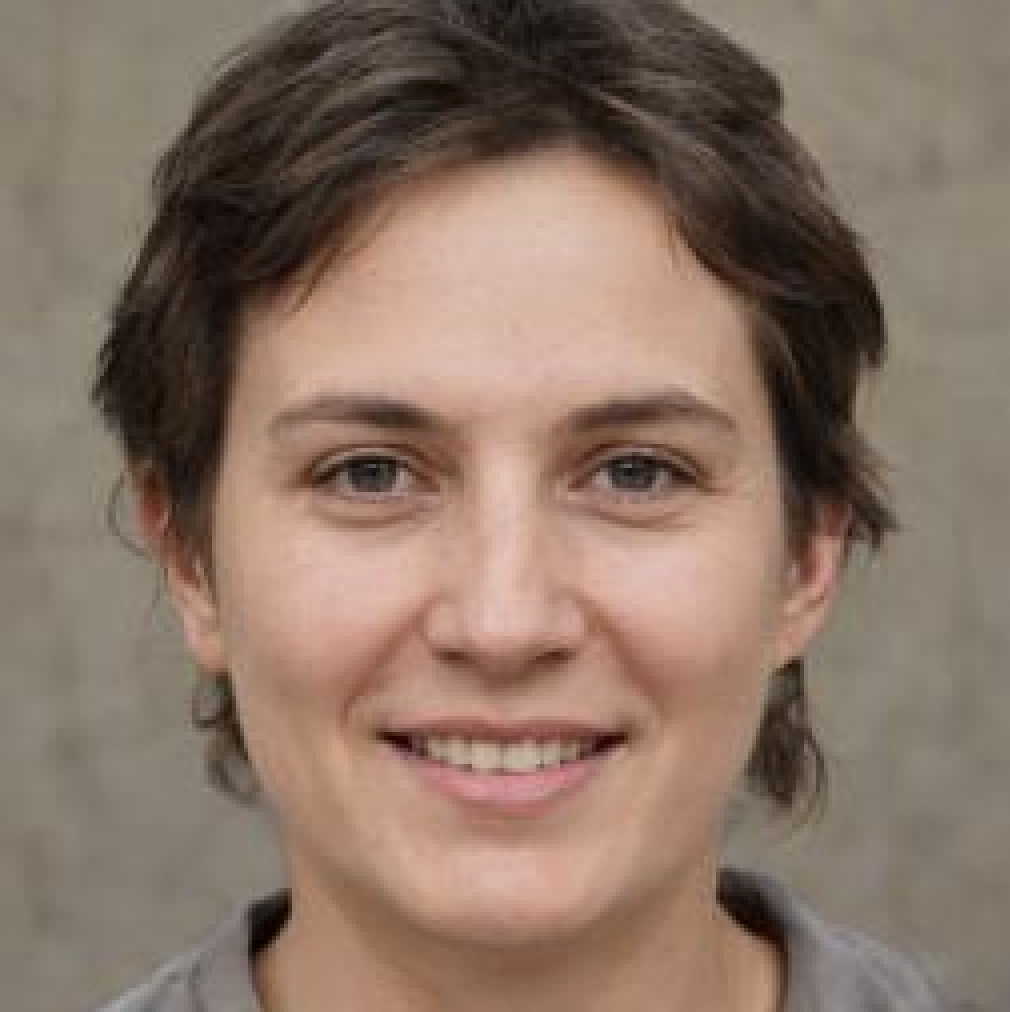
\includegraphics[scale=0.2]{figures/avg_image.png}
  \caption{Average image used}
  \label{fig:Average image}
\end{figure}
%\subsection{Training}
% HO UN PEZZO DI SCRITTE SULLE NOTE NEL CASO VOLESSI AGGIUNGERE L'ADDESTRAMENTO FATTO SUL PRIMO DATASET PERò NON HO I RISULTATI FINALI
\\
Initially, the first dataset was used to train the network for a duration of three days. However, the results obtained from this training were not up to the expected standards. Subsequently, the second dataset was employed for training the network from scratch for three days. This resulted in a noticeable improvement in the network's performance. Nevertheless, some crucial features were still missing from the output when testing the model. For example, when the sketch presented a person with the beard in the generated image this detail did not appear, and the same happened for details like dimples and wrinkles. To address this, the network was further trained for other three days. Indeed, the model was trained for a total of 70'000 iterations and the end result was a trained generative adversarial network capable of producing realistic face images when conditioned on input sketches.\\
In fig.~\ref{fig:training results} it can be seen the result of the training phase.
\begin{figure}[htbp]
    \centering
    \subfloat[][\emph{Train: 30'000-th iteration}]
    {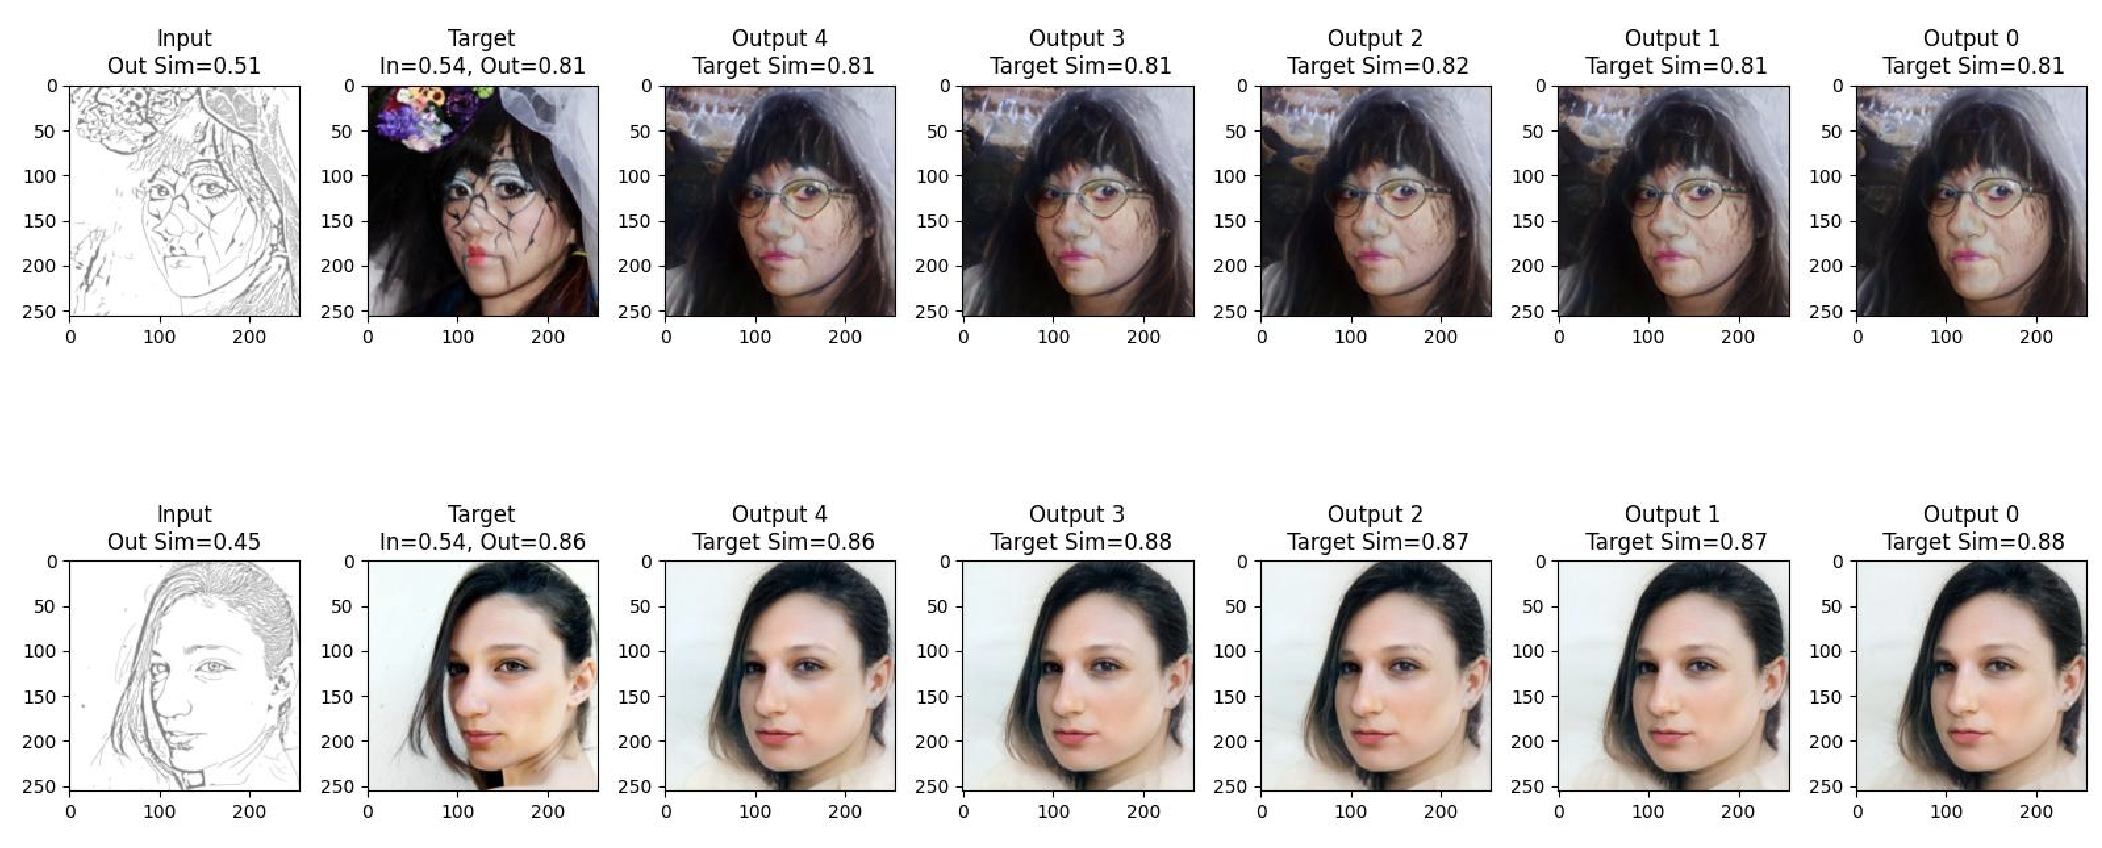
\includegraphics[width=.8\textwidth]{figures/train3000-2db.png}} \quad
    \subfloat[][\emph{Train: 70'000-th iteration}]
    {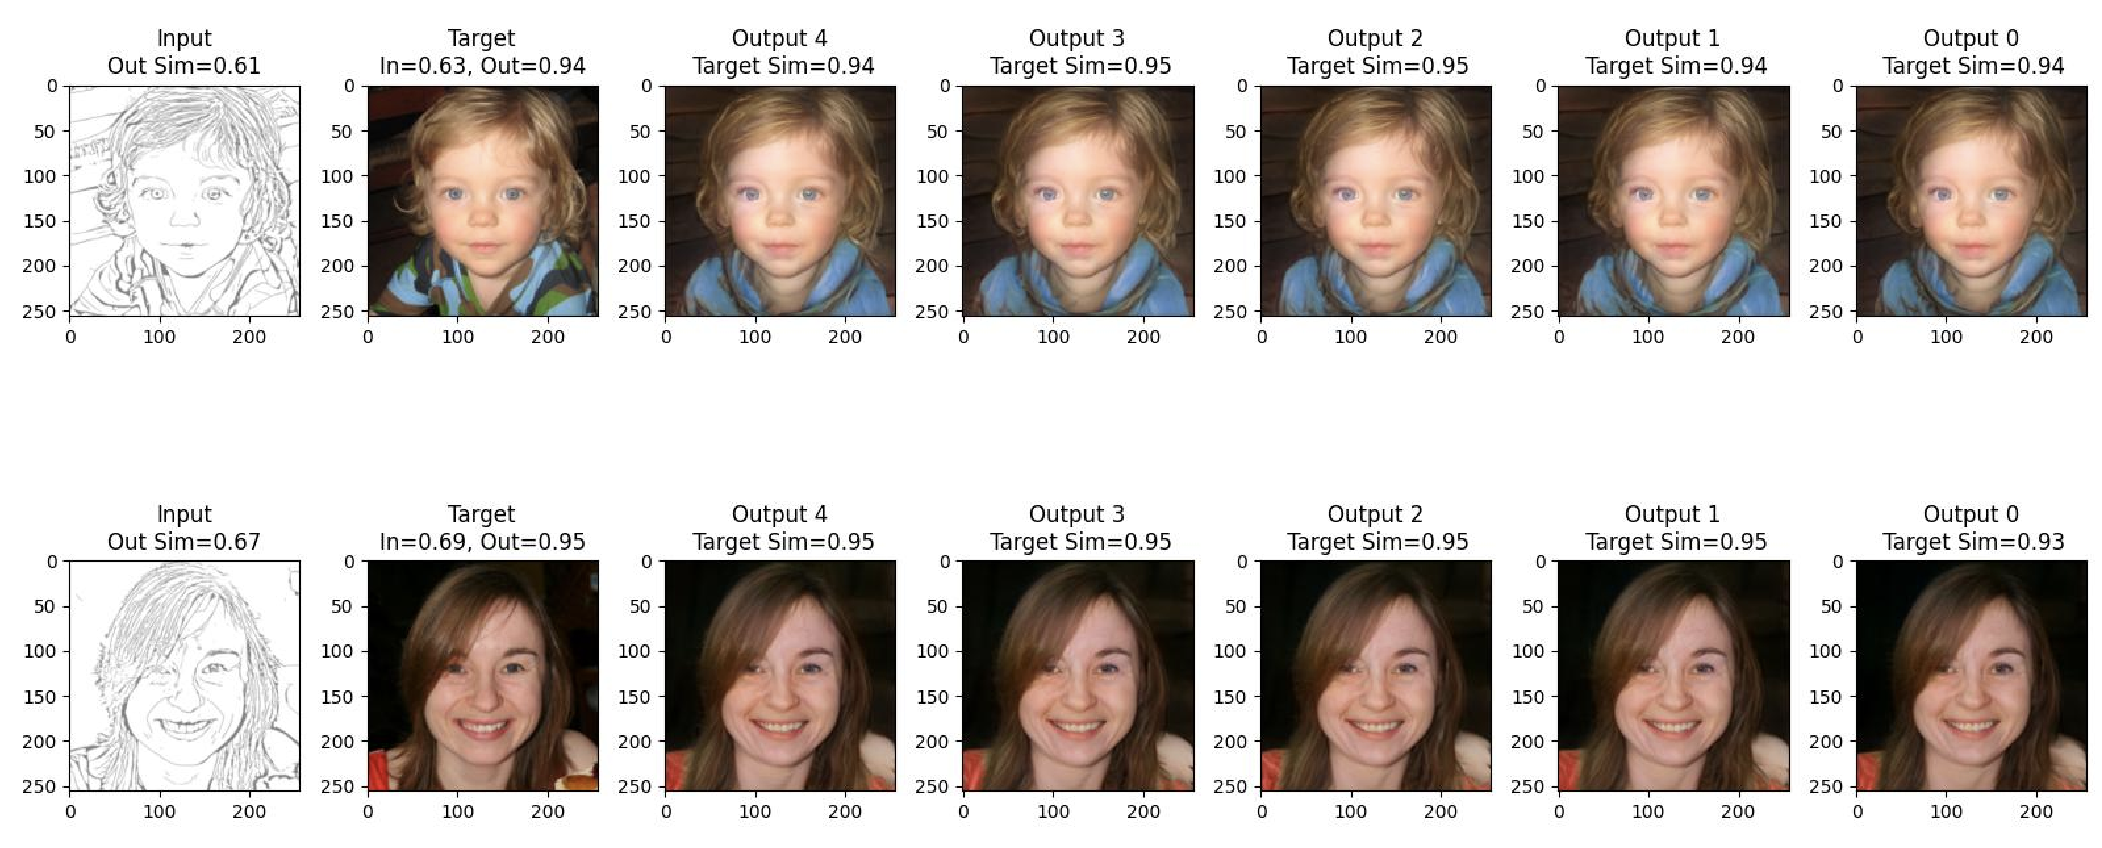
\includegraphics[width=.8\textwidth]{figures/train70000-2DB.png}}\\
    \caption{Training results}
    \label{fig:training results}
\end{figure}
%%%
%
%
\subsubsection{Testing's setup}
\label{sec:testing setup}
For the purpose of generating synthetic images with the trained model, a graphical user interface has been developed, along with a client-server architecture. All these three are done in Python using the \textit{RPyC} library. This setup enables the model to be tested in a convenient and efficient manner, as the graphical interface provides an easy-to-use interface for inputting data and analysing the results, while the client permits to test the model from the command line inputting existing sketches.\\ \\
%
%\subsubsection{Graphical user interface}
\textbf{Graphical user interface}\\
%\label{sec:graphical interface}
The graphical user interface was done using \textit{Tkinter} library, which allows users to draw on a canvas using a black pen. Additionally, users can use a rubber to delete portions of the sketch, or directly remove the previous inserted lines using the “undo” button, or also clear the canvas, with the “delete” button, and start again from scratch. The rubber and the pen can vary in thickness between 1 (thinner) and 10 (thicker). Furthermore, three dashed lines are present, one is vertical in the centre of the interface and the other two are horizontal and placed at eye and chin level. Those lines guide the users in positioning main facial features like the eyes, nose, and mouth. The fig.~\ref{fig:Graphical interface} shows a sketch drawn on the interface.\\
Once the “send” button is pressed, the drawing is sent to the server.
To start the interface, the following command has to be executed.
\begin{lstlisting}[numbers=none]
    python interface.py [-h] [-p PORT] [-a HOST]
    Options:
      -h                this help
      -p PORT           remote server port, default: 18862
      -a HOST           remote server address, default: 140.105.164.230
\end{lstlisting} 
\begin{figure}[htbp]
\centering
  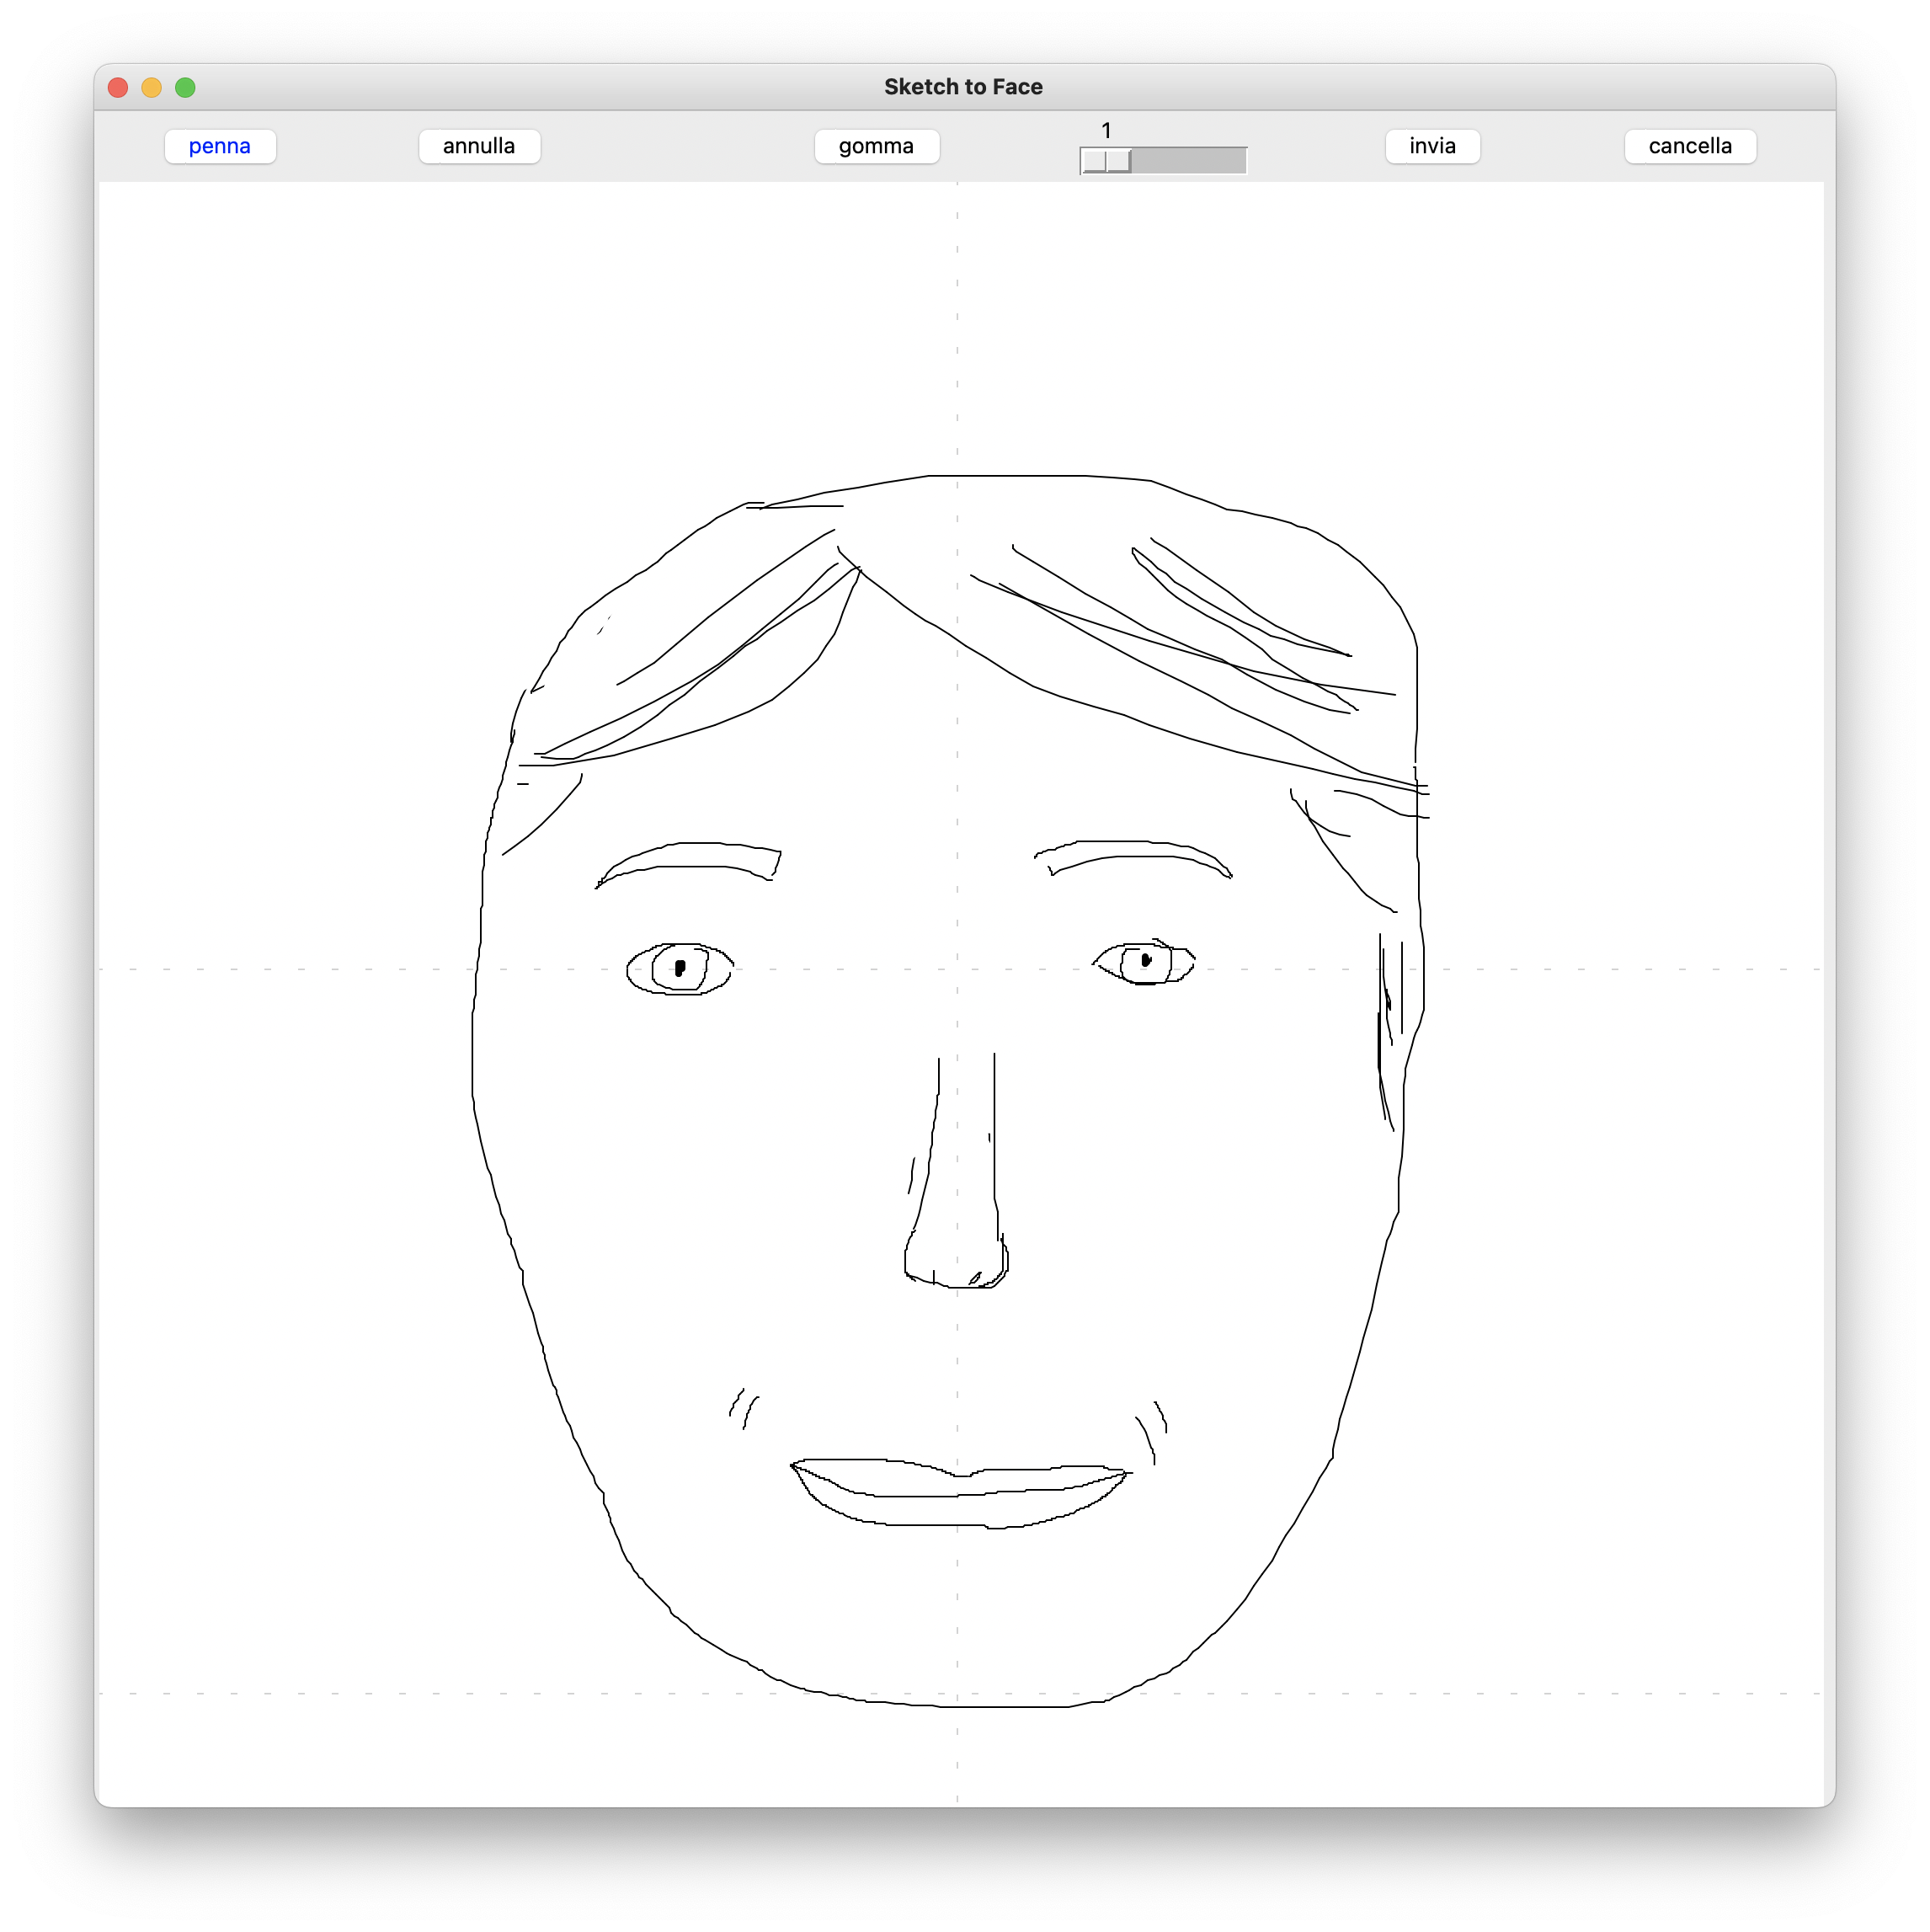
\includegraphics[scale=0.15]{figures/interface.png}
  \caption{Graphical interface}
  \label{fig:Graphical interface}
\end{figure}
%% 
%\subsubsection{Client architecture}
\textbf{Client architecture} \\
An image can also be generated from the command line typing:
\begin{lstlisting}[numbers=none]
    python client_next.py [-h] -i IMAGE [-o OUT] [-p PORT] [-a HOST]
    Options:
      -h                this help
      -i IMAGE          input image
      -o OUT            output file, default: output_results.jpg
      -p PORT           remote server port, default: 18862
      -a HOST           remote server address, default: 140.105.164.230
\end{lstlisting}
The input sketch has to be specified, while there are other parameters that can be set are not mandatory.\\ \\
% It opens an image file using the Pillow library and converts it to RGB format. The image is then saved to a buffer and converted to a string. The code then uses the rpyc.connect() method to connect to the server at the specified host name and port. It then calls the exposed\_get\_face method from the root object on the remote server and passes the image string to it. The response from the server is received as a base64-encoded string and is decoded to an image, which is then saved to the specified file.\\
%
%\subsubsection{Server architecture}
\textbf{Server architecture}\\
To be able to generate the image based on the sketches the server has to be up, therefore the following command has to be executed otherwise it will not be possible to generate images.
\begin{lstlisting}[numbers=none]
    python server_next.py [-h] -m MODEL [-t TYPE] [-p PORT]
    Options:
      -h                this help
      -m MODEL          pretrained model
      -t TYPE           type of the mode, either psp or e4e, default: psp
      -p PORT           remote server port, default: 18862
\end{lstlisting}
Once an image is sent to the server, the restyle encoder is applied to generate the output image, which is then sent back as a byte stream and then saved as a PNG image. The server allows also multiple clients since it used the \textit{ThreadedServer} class of \textit{RPyC}.
 % CAP 5
\newpage
\section{Evaluation and results}
\label{sec:evaluation}
Throughout this thesis, a few experiments were conducted to evaluate the performance of the trained model in terms of quality of the generated images. The results of these experiments have been consolidated in this section.

\noindent To assess the quality of conditional image synthesis, a survey was prepared, comprising \num{20} distinct sketches, each associated with four images.
Among the four images, one was generated from the sketch, while the other three were selected from the FFHQ dataset based on the similarity metric described in~\ref{sec:xcos}.
The FFHQ dataset has been chosen due to the fact that it was the dataset used to train the model.
The \num{20} images were chosen from \num{3256} sketches done by people during a scientific research festival on a graphic tablet.
These sketches were made on the graphical interface described in~\ref{sec:testing setup}.

\noindent In the process of collecting the sketches, it was observed that if the size of the sketches was too small or if the position of the eyes was too high or low on the graphical interface, the resulting generated image did not accurately resemble the original sketch.
To address this issue, two horizontal lines and a vertical line, discussed in section~\ref{sec:testing setup}, were added.
This allowed individuals to have a better understanding of the appropriate size of the sketch and the correct placement of the main facial characteristics to ensure accurate image generation.
Furthermore, it has been observed that the sketches made using a pen with a thickness greater than three tend to result in bad images, despite the talent of the artist who created the sketch.

\noindent Fig.~\ref{fig:disappointing sketch small} shows an instance of unsatisfactory outcome achieved from a highly realistic sketch, which was produced using a very small scale.
%or with a pen that was excessively thick.
\begin{figure}[htbp]
  \centering
  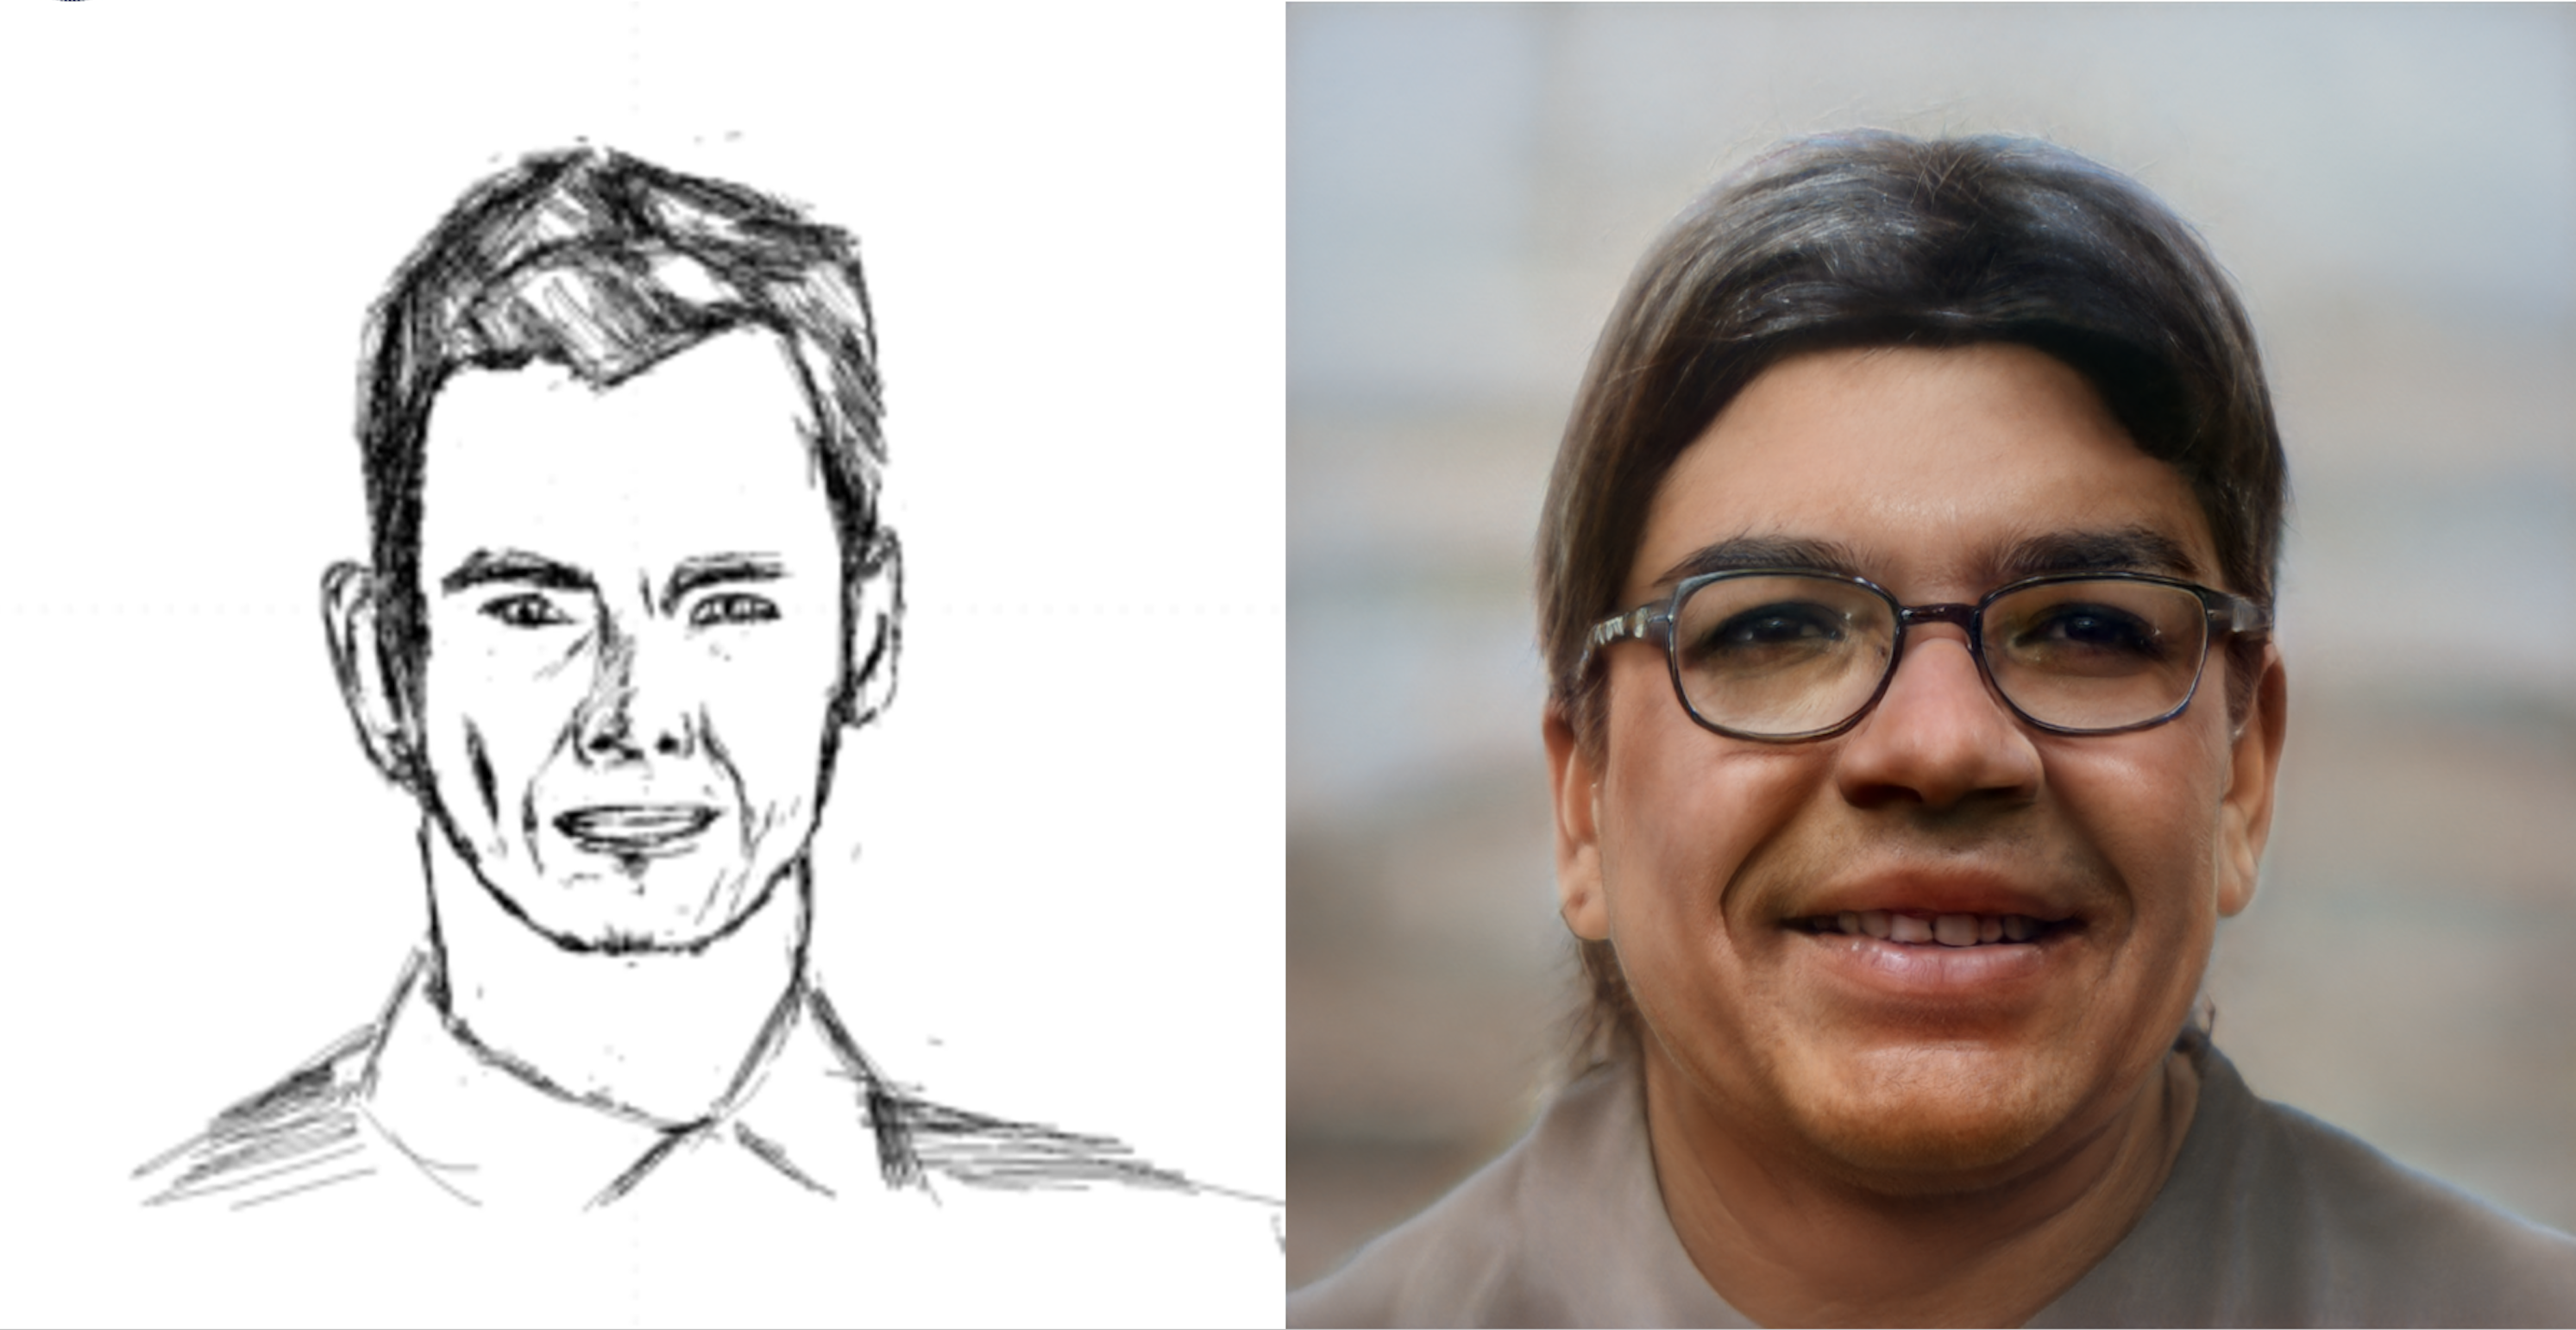
\includegraphics[scale=0.15]{figures/badResult1.png}
  \caption{Disappointing result generated from a sketch too small}
  \label{fig:disappointing sketch small}
\end{figure}

\noindent As illustrated in Fig.~\ref{fig:result thick pen}, the use of a pen too thick can have a negative effect on the generated images, for example it can generate unrealistic hair and colours. However, upon closer examination of the generated image, it can be observed that certain details of the original sketch are still present. 
\begin{figure}[htbp]
  \centering
  \includegraphics[scale=0.15]{figures/badResult.png}
  \caption{Result obtained from a sketch made with a thick pen}
  \label{fig:result thick pen}
\end{figure}
%

\noindent Impressive results can be achieved when talented people create the sketches. It is worth noting that the success of the generated image is highly dependent on the quality of the input sketch. Where the term “quality” is related to the dimension of the sketch and the pen's thickness.
Therefore, it is essential to carefully consider the conditions under which the sketch is created to obtain optimal results. An example of a very breathtaking result can be seen in Fig.~\ref{fig:impressive result}, while Fig.~\ref{fig:result simple sketch} depicts a straightforward input sketch and its corresponding generated image that exhibits noticeable similarity.
\begin{figure}[htbp]
  \centering
  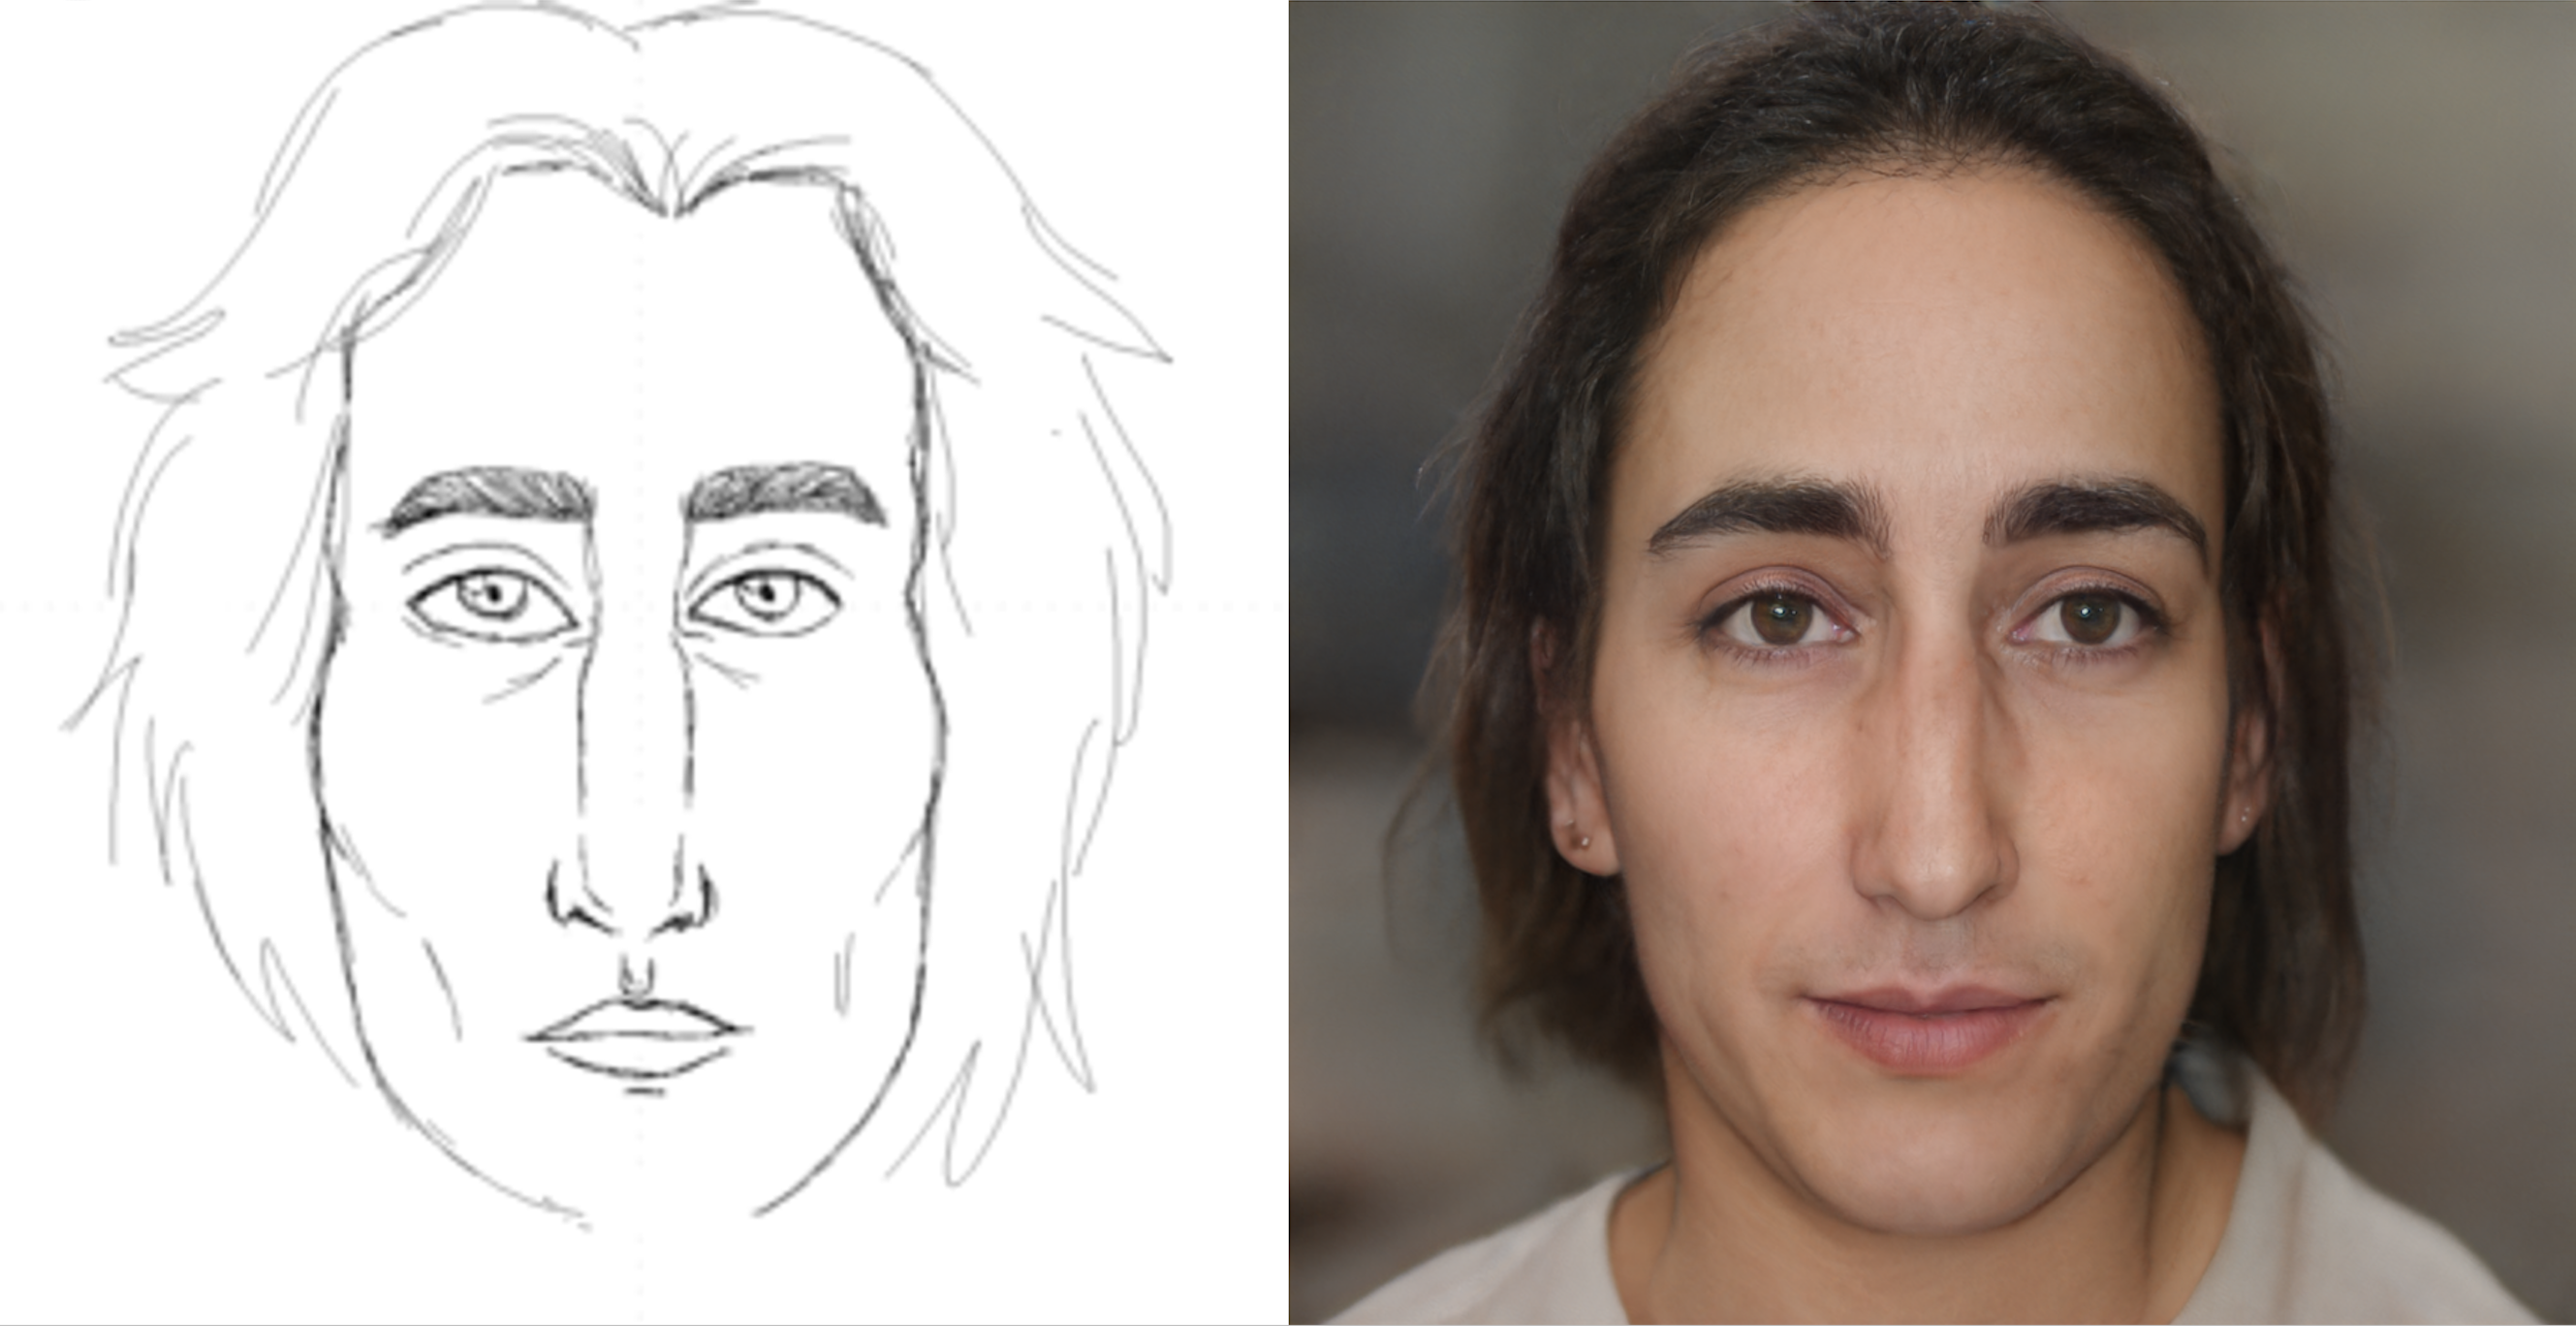
\includegraphics[scale=0.15]{figures/goodResult.png}
  \caption{Impressive result of an image generated from a sketch}
  \label{fig:impressive result}
\end{figure}
\begin{figure}[htbp]
  \centering
  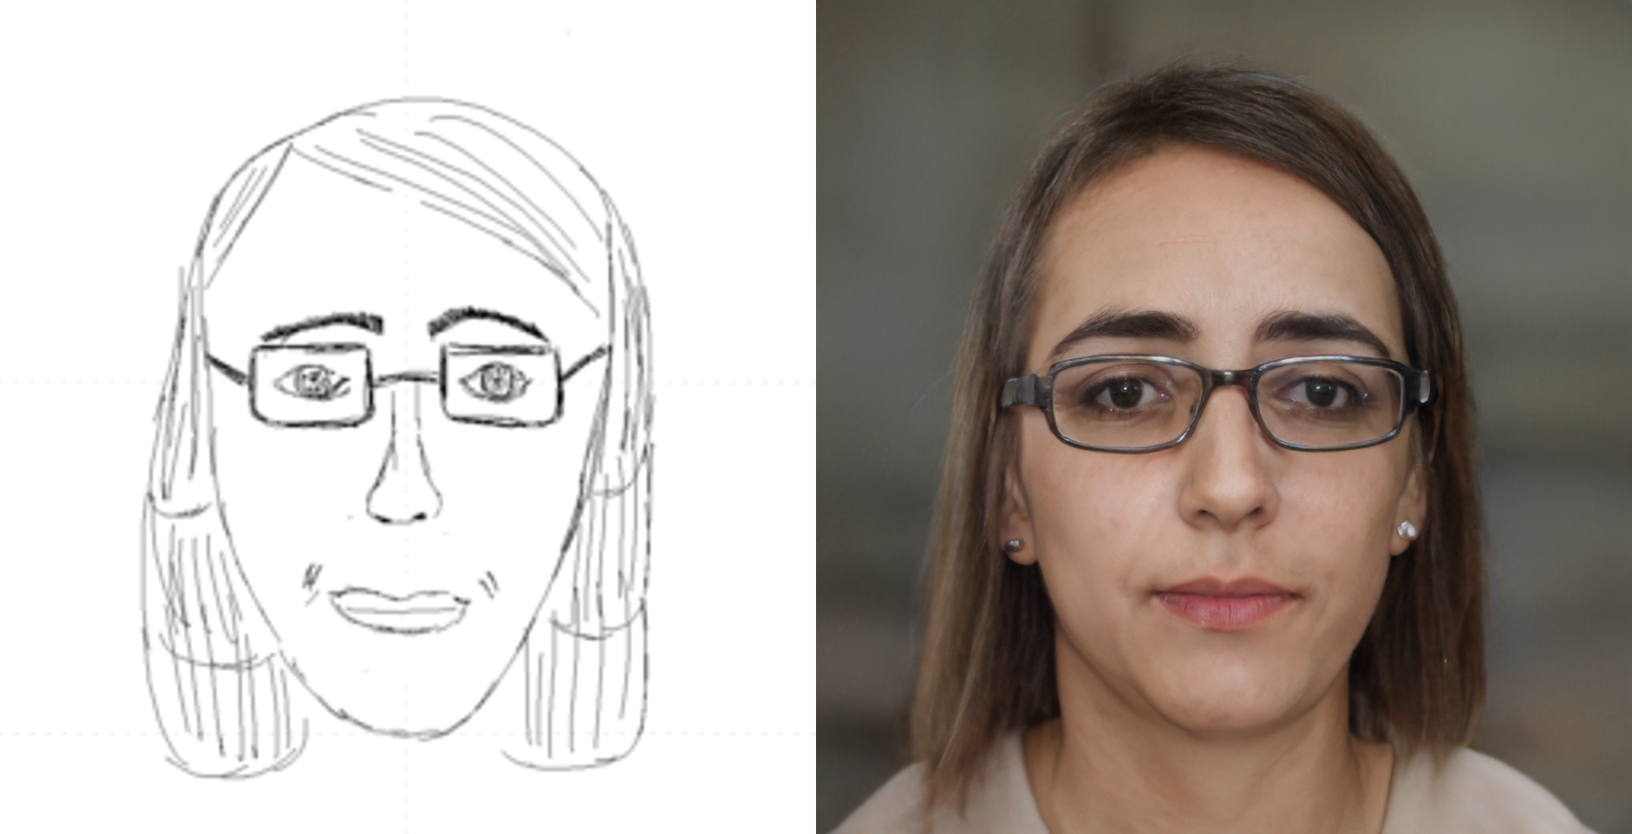
\includegraphics[scale=0.25]{figures/goodResult-simpleSketch.png}
  \caption{Result of an image generated from a simple sketch}
  \label{fig:result simple sketch}
\end{figure}
%

\noindent Given the diverse range of people who contributed to the sketch dataset, consisting of individuals with varying age groups and drawing abilities, it became necessary to filter out sketches that were unrealistic. Furthermore, some sketches displayed minor differences, as shown in Fig.~\ref{fig:similar sketches}, or only portrayed the outline of the face without any distinguishable feature (Fig.~\ref{fig:discarded images}).
\begin{figure}[htbp]
    \centering
    \subfloat[][\emph{ }]
    {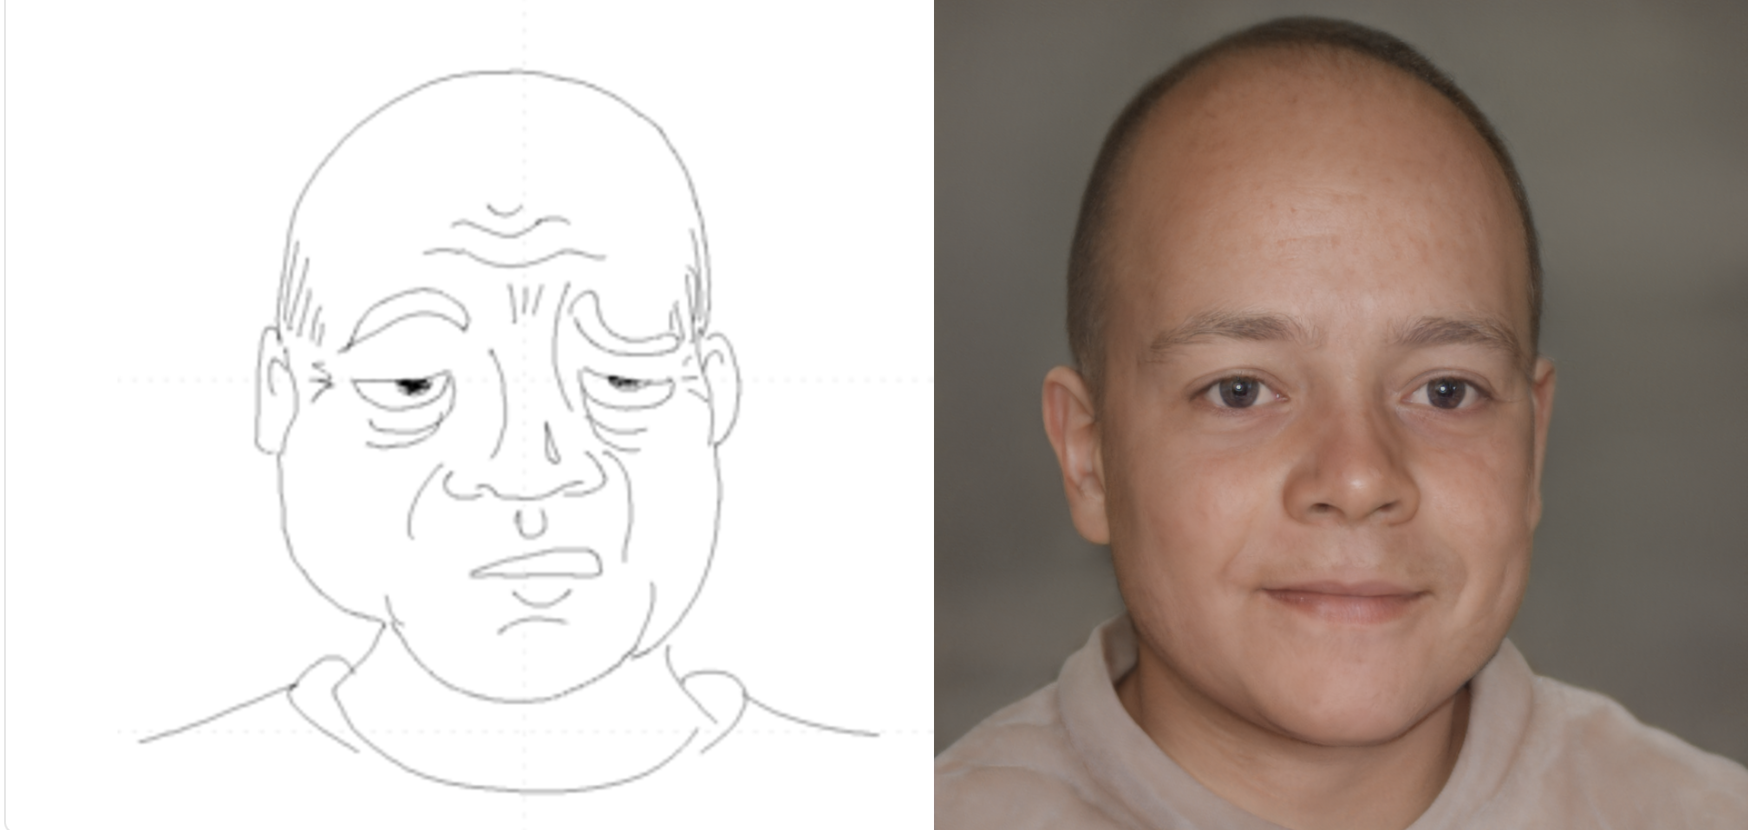
\includegraphics[width=.4\textwidth]{figures/similarSketch2.png}} \quad
    \subfloat[][\emph{}]
    {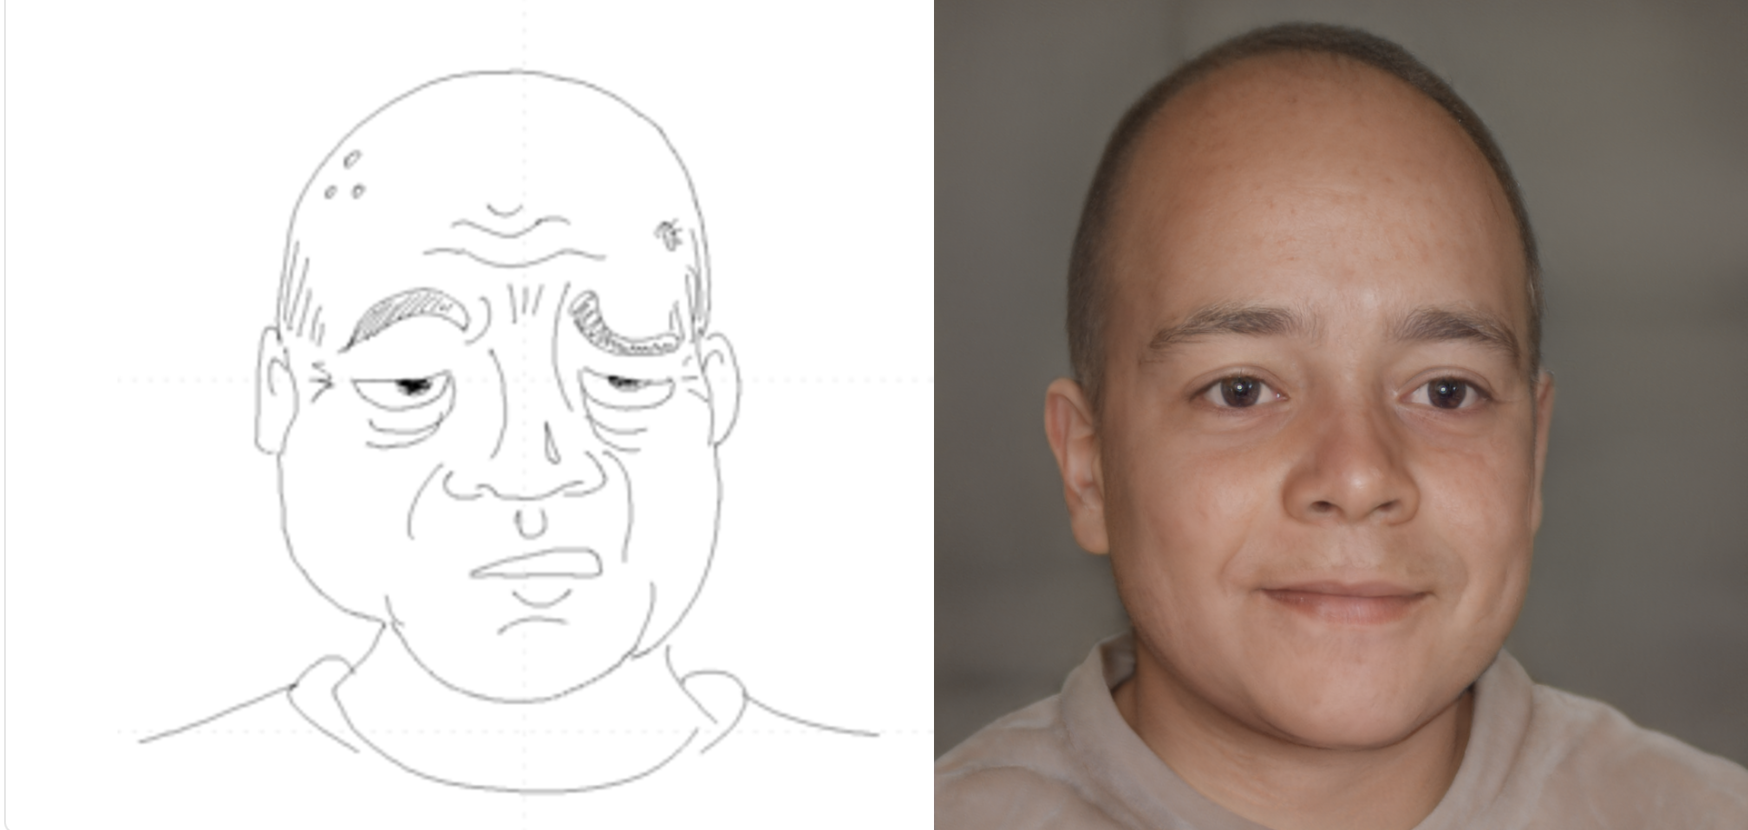
\includegraphics[width=.4\textwidth]{figures/similarSketch1.png}}
    \caption{Examples of two similar sketches}
    \label{fig:similar sketches}
\end{figure}
\begin{figure}[htbp]
    \centering
    \subfloat[][\emph{Empty sketch}]
    {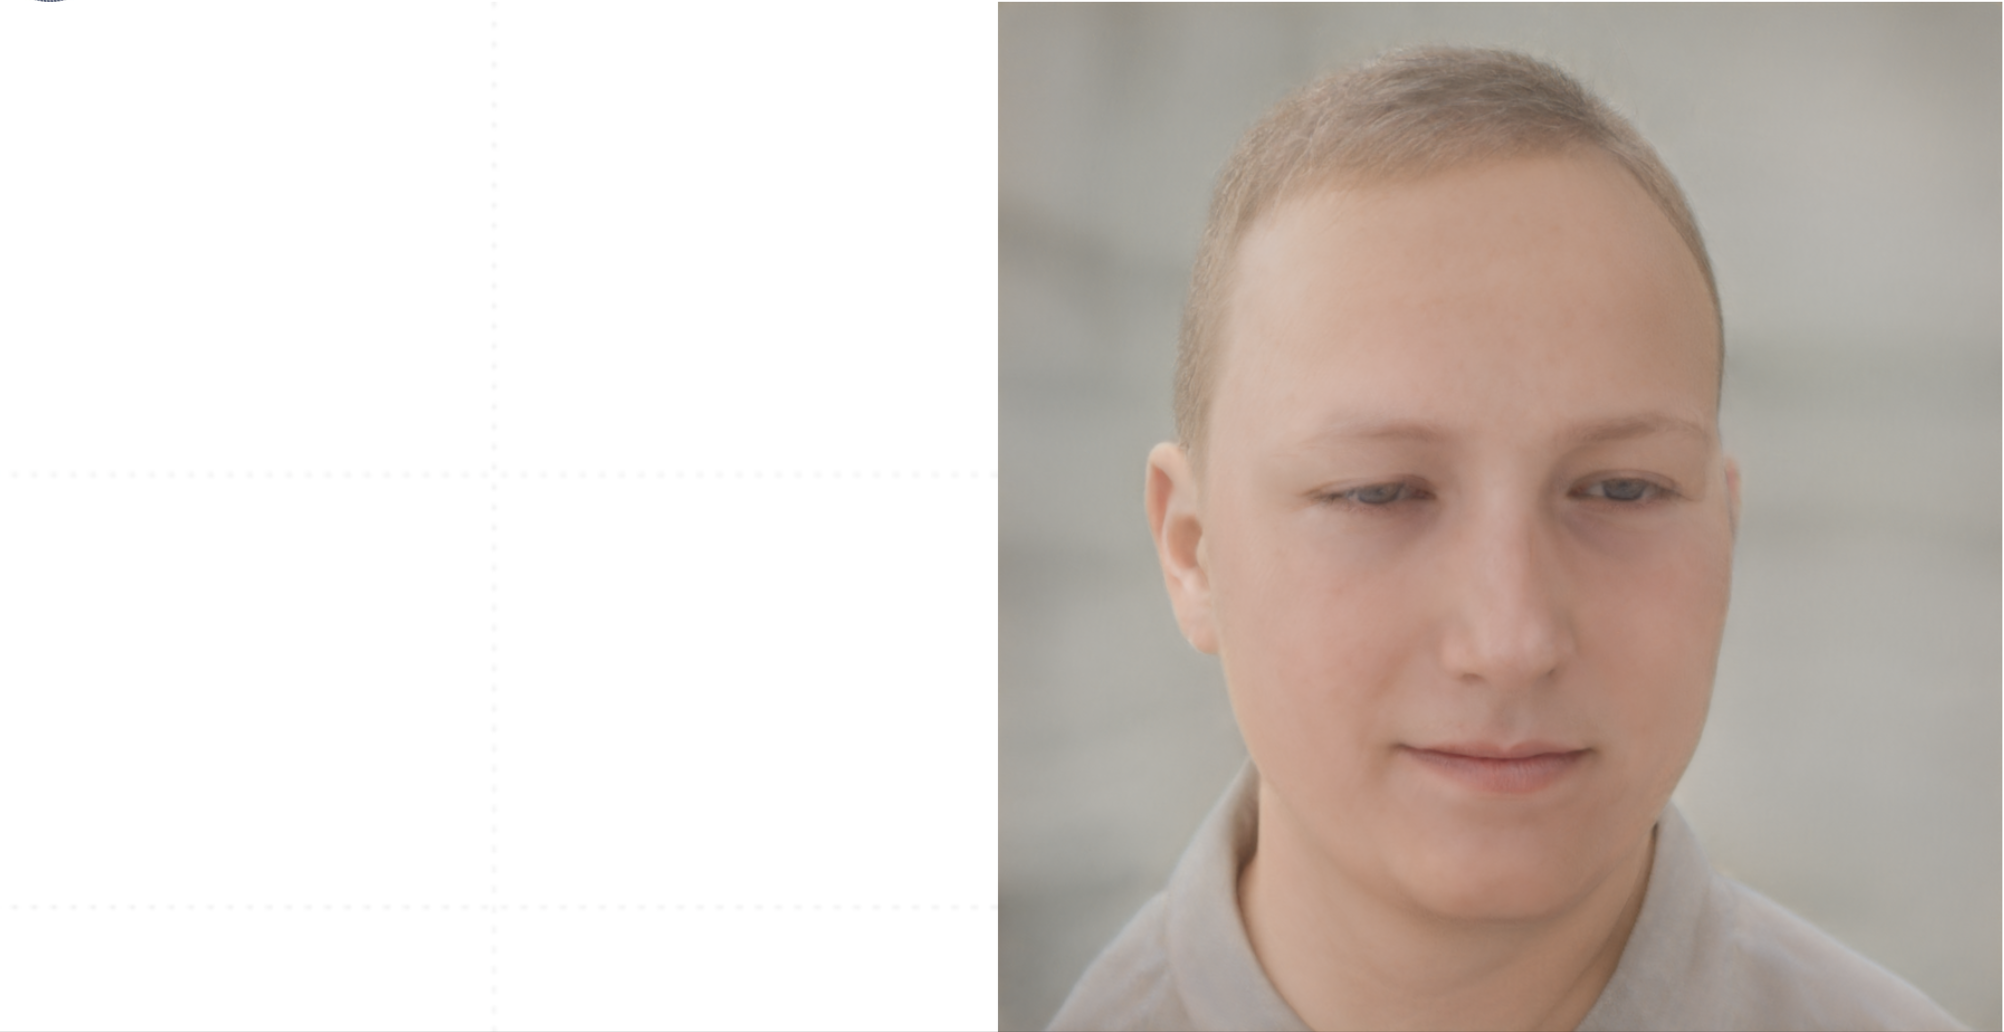
\includegraphics[width=.4\textwidth]{figures/emptySketch.png}} \quad
    \subfloat[][\emph{Sketch with just the contour of the face}]
    {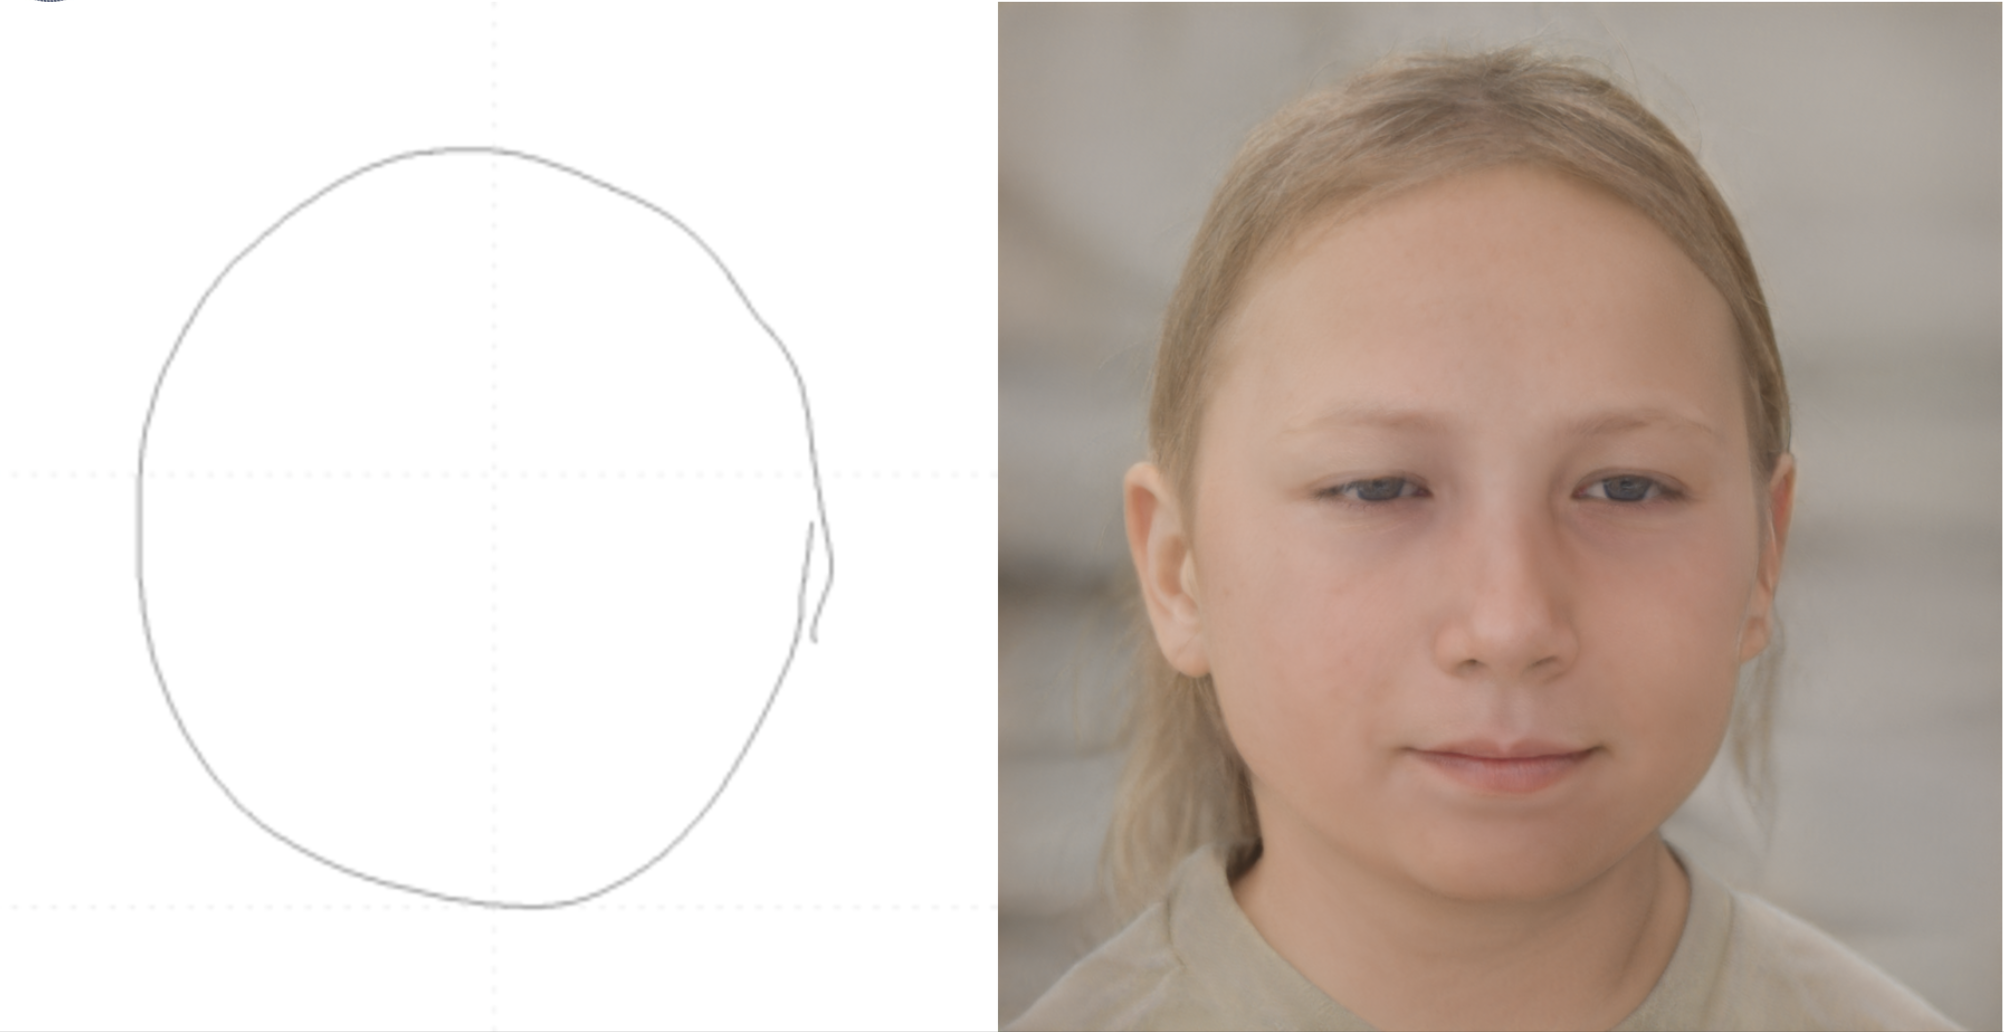
\includegraphics[width=.4\textwidth]{figures/sketchOnlyContour.png}}\\
    \subfloat[][\emph{Sketch done with a thick pen}]
    {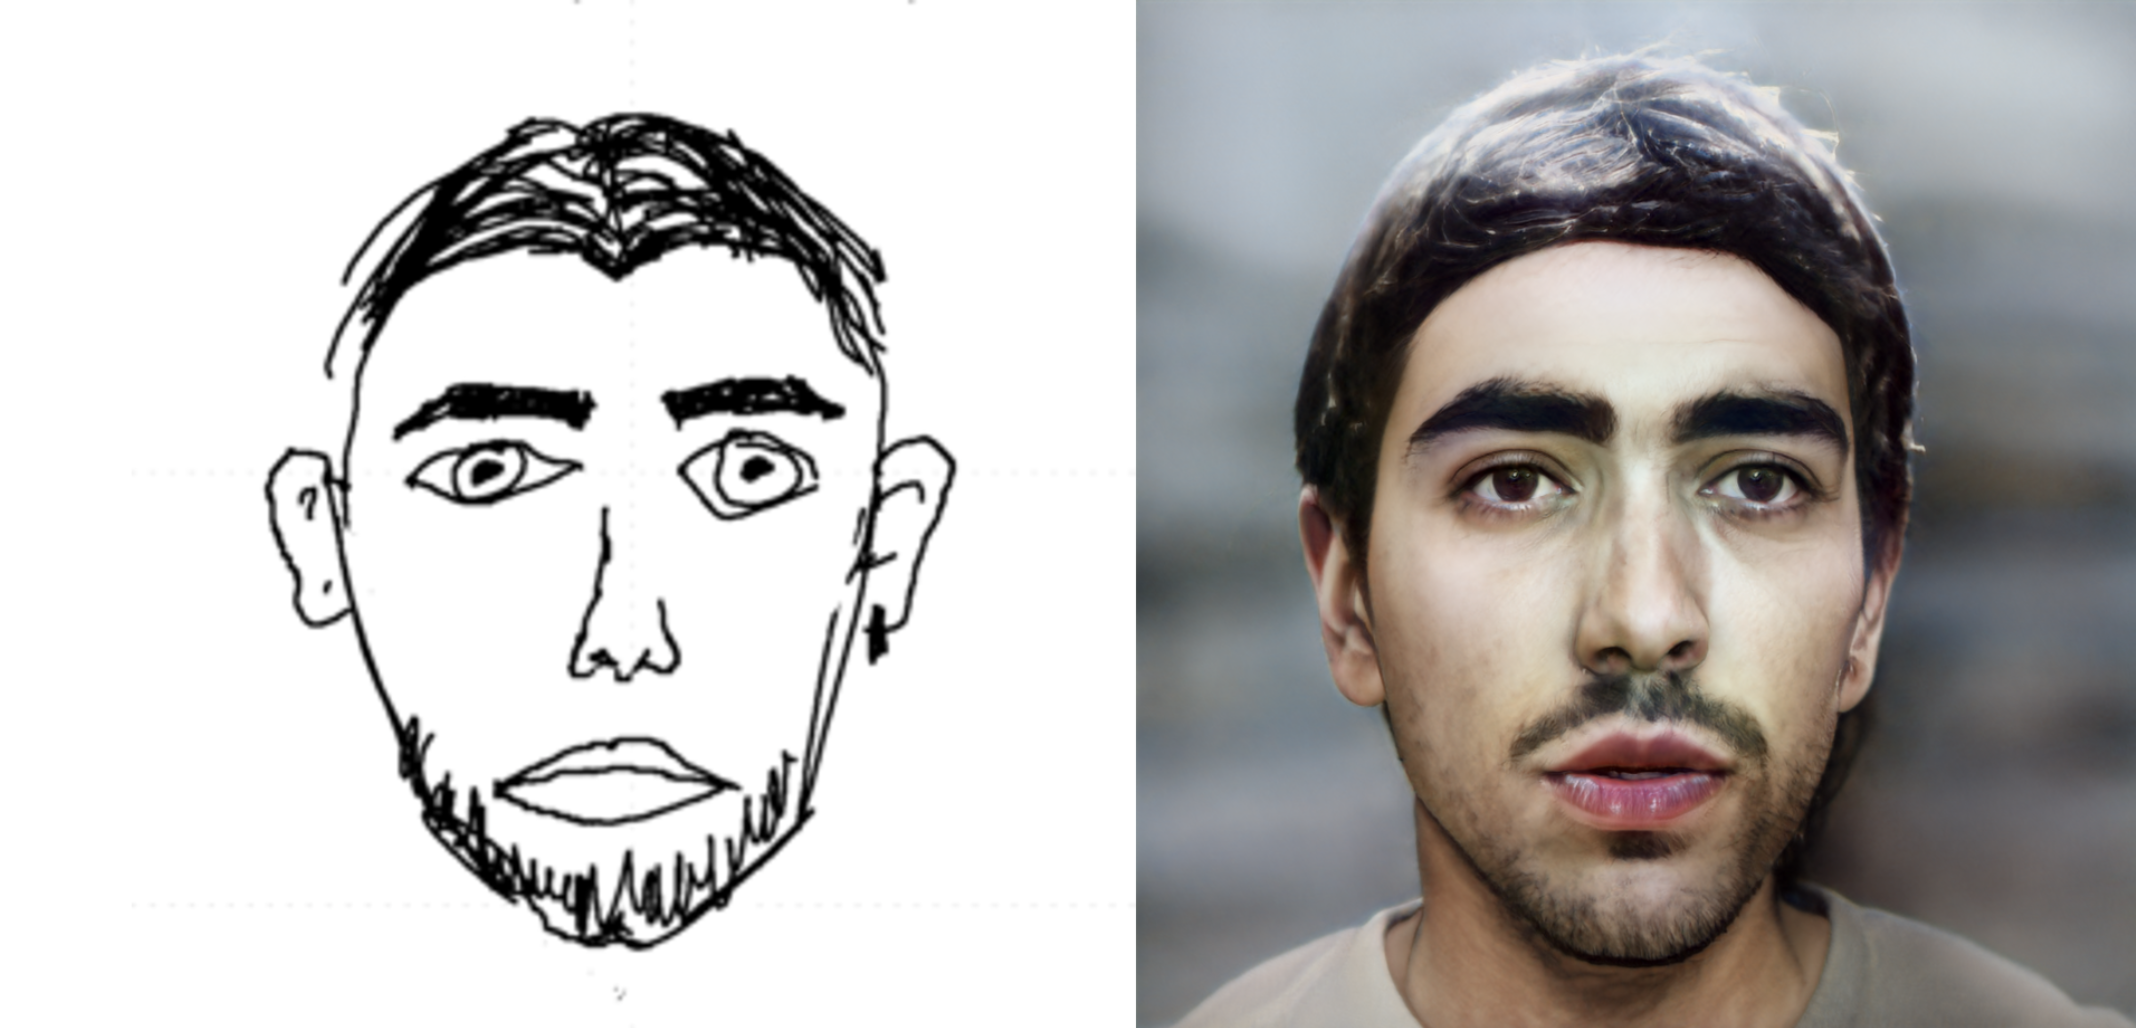
\includegraphics[width=.4\textwidth]{figures/thickPenSketch.png}}
    \caption{Examples of discarder images}
    \label{fig:discarded images}
\end{figure}

\noindent Therefore, the initial set of sketches was manually processed to remove such sketches, leaving only the more realistic ones. Subsequently, the remaining images underwent further analysis, and the poorest sketches were discarded. Finally, the xCos metric was applied to the filtered dataset to identify the most similar images to the sketches.


\noindent The survey was built in such a way that \num{5} random images out of the \num{20} are displayed. The survey's participants were instructed to choose the image that in their opinion had inspired the realisation of the sketch. An example of how the images are displayed in the survey is shown in Fig.~\ref{fig:survey images}.
\begin{figure}[htbp]
    \centering
    \subfloat[][\emph{ }]
    {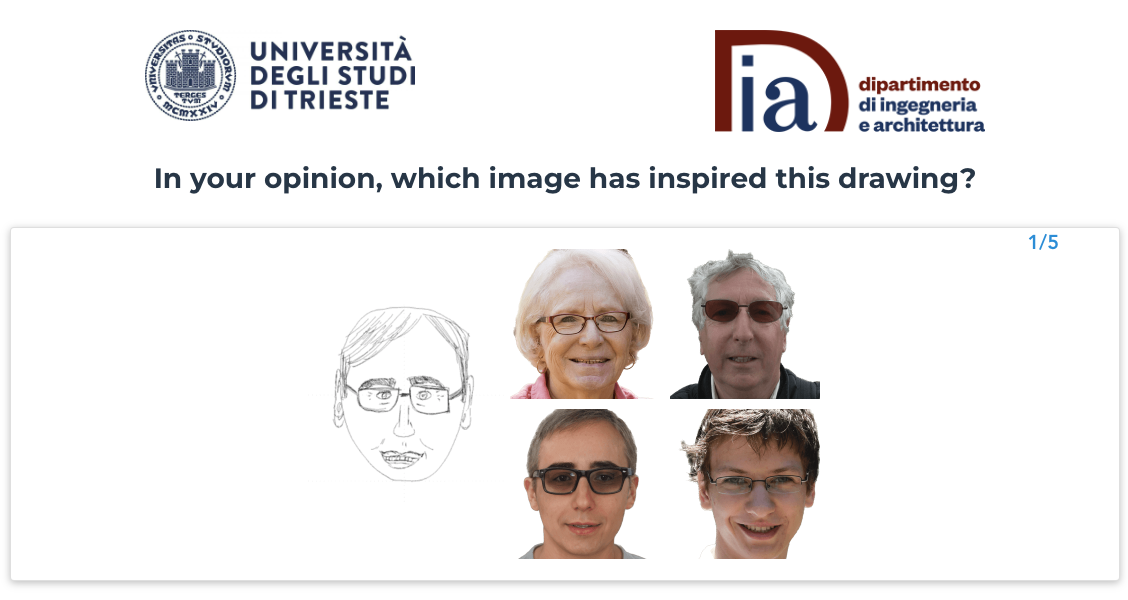
\includegraphics[width=.8\textwidth]{figures/survey1.png}} \quad
    \subfloat[][\emph{}]
    {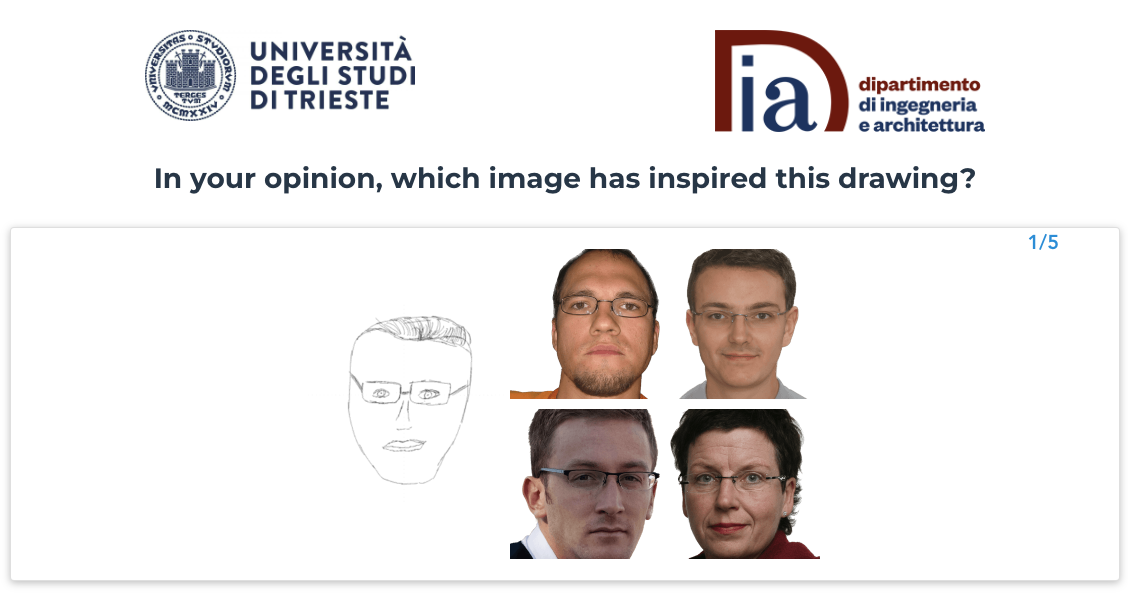
\includegraphics[width=.8\textwidth]{figures/survey2.png}}
    \caption{Examples of the structure of the survey}
    \label{fig:survey images}
\end{figure}
%

\subsection{Survey's results}
\label{sec:survey results}
Out of the \num{202} responses collected from the survey,  only \num{155} were considered for the analysis because the remaining \num{47} came from people try to complete the survey a second time.


\noindent Figure~\ref{fig:bar plot with correct/incorrect responses} (a) and (b) provide an overview of the results obtained from the survey. The figure displays the total number of correct and incorrect responses for each sketch, indicated by green and red bars, respectively. The sketches are labelled on the x-axis.

\begin{figure}[!b]
  \centering
  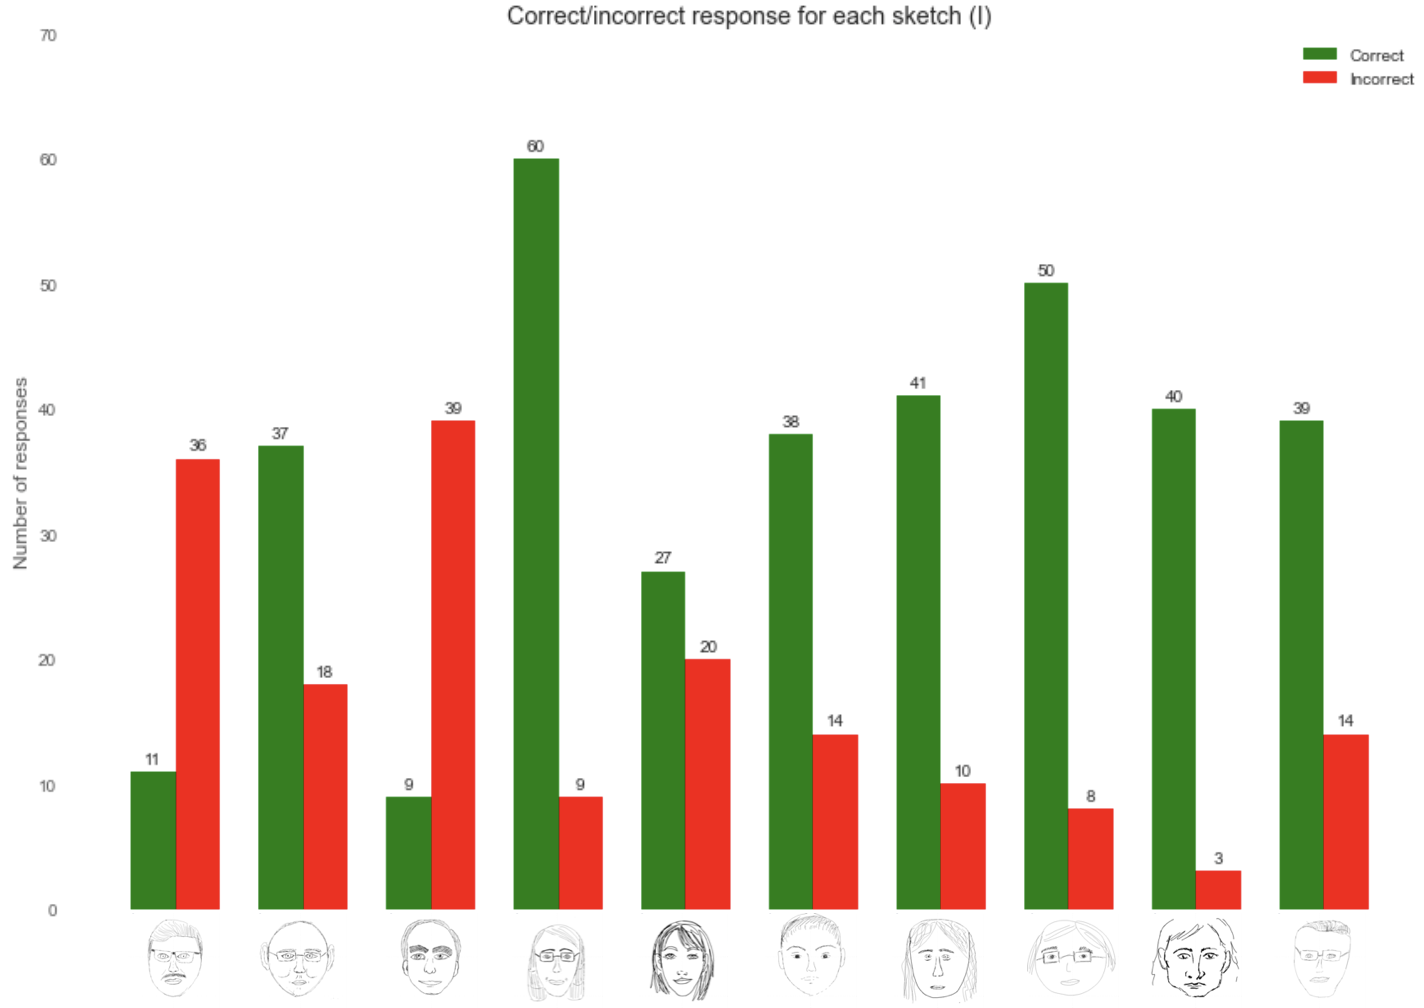
\includegraphics[width=1\textwidth]{figures/RISULTATI/correctIncorrectResponses-1.png}
  \caption{Results for the first \num{10} sketches (a).}
  \label{fig:bar plot with correct/incorrect responses}
\end{figure}

\begin{figure}[ht]
  \ContinuedFloat
  \centering
  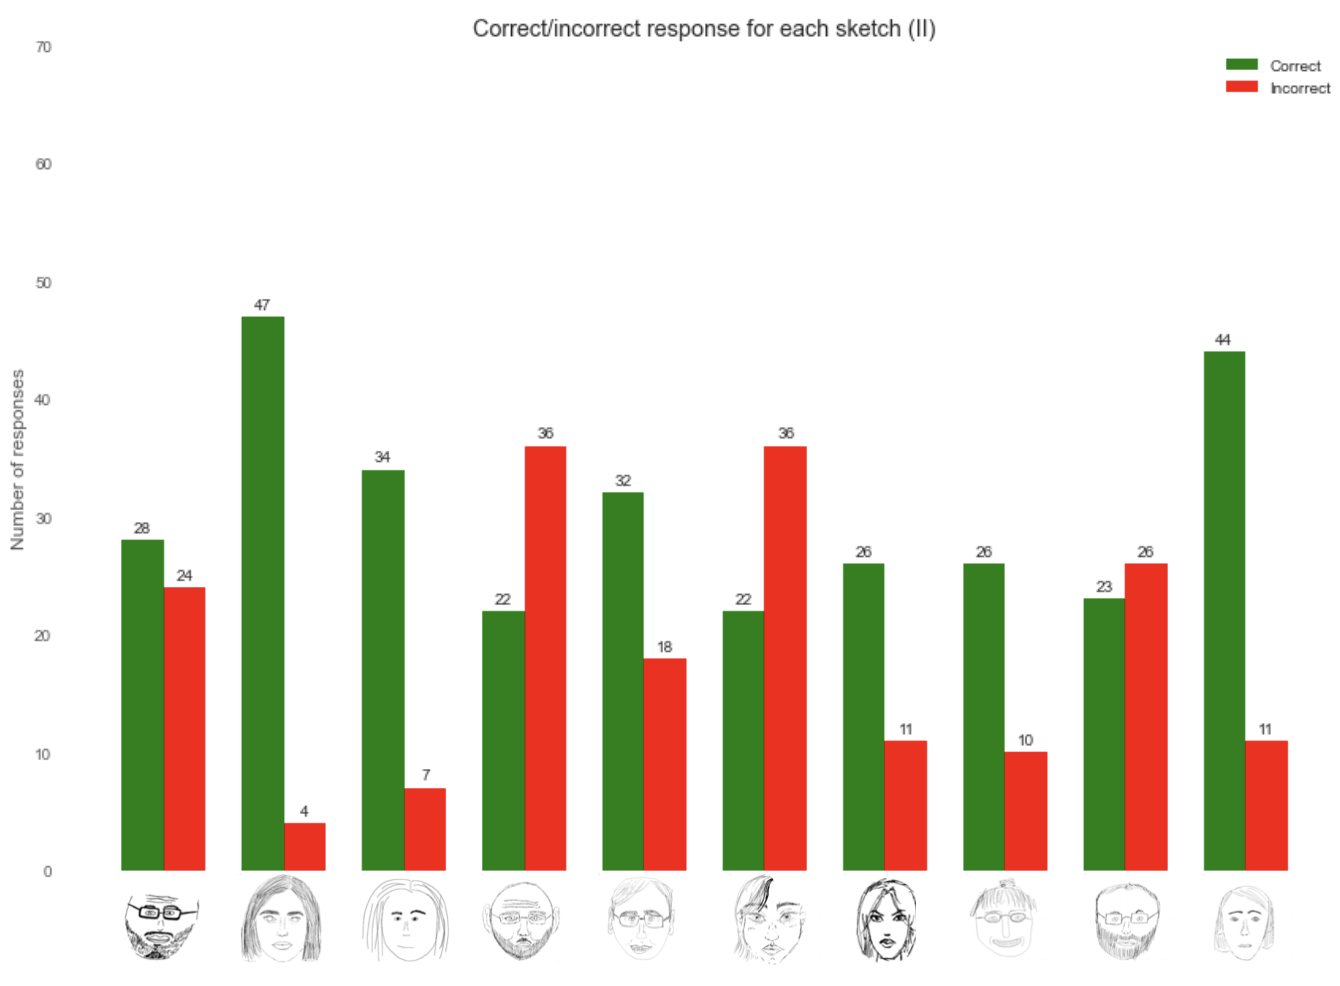
\includegraphics[width=1\textwidth]{figures/RISULTATI/correctIncorrectResponses-2.png}
  \caption{Results for the second \num{10} sketches (b).}
  \label{fig:bar plot with correct/incorrect responses}
\end{figure}

%\begin{figure}[htbp]
% \centering
%    \subfloat[][\emph{Results for the first \num{10} sketches}]
%    {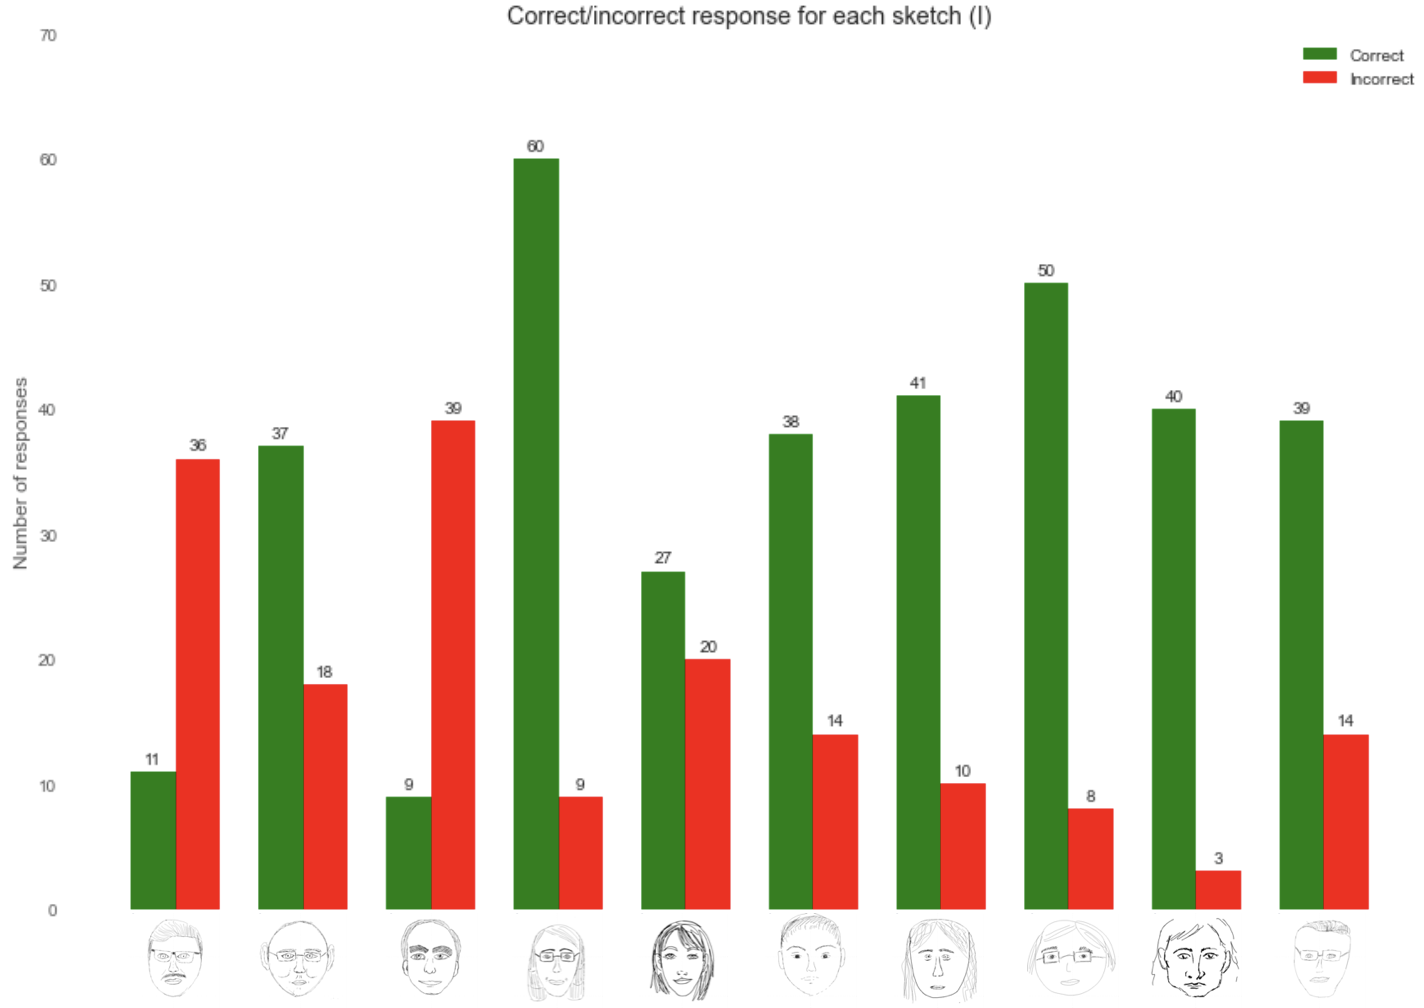
\includegraphics[width=.8\textwidth]{figures/RISULTATI/correctIncorrectResponses-1.png}} \\
%    \subfloat[][\emph{Results for the second \num{10} sketches}]
%    {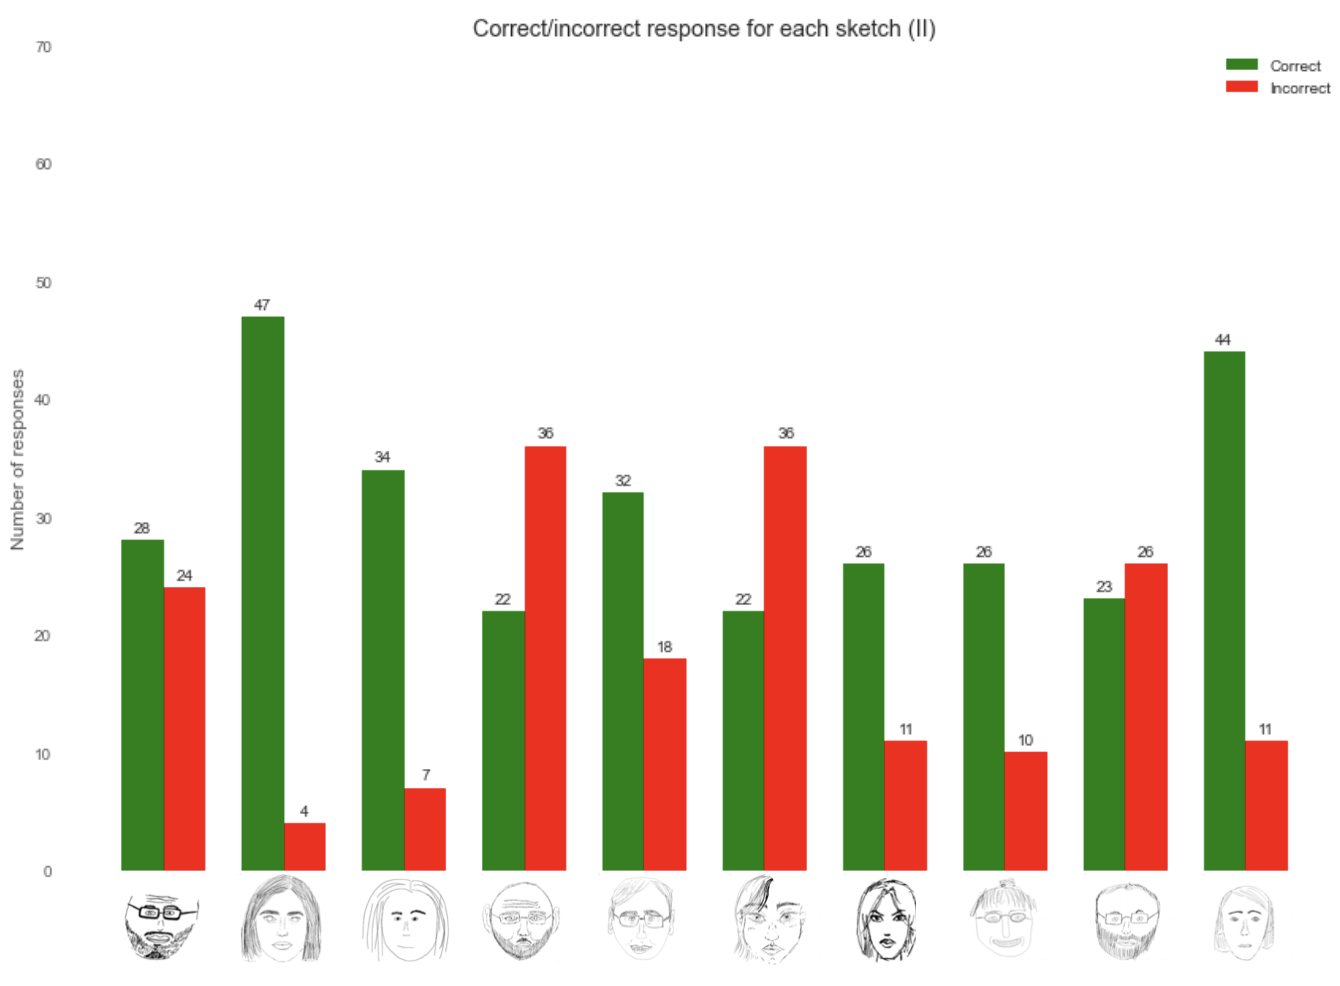
\includegraphics[width=.8\textwidth]{figures/RISULTATI/correctIncorrectResponses-2.png}}
%    \caption{}
%    \label{fig:bar plot with correct/incorrect responses}
%\end{figure}

   

\noindent Table~\ref{tab:responses summary} shows the percentage of correct responses and the average response time in seconds for each sketch in the survey.
\begin{table}[!ht]
\begin{center}
    \begin{tabular}{lcc}
    \textbf{SketchID} & \textbf{\% correct responses} & \textbf{average time (s)} \\
    0 & 23.4 \%  & 19.79 \\
    1 & 67.3 \%  & 14.13 \\
    2 & 18.8 \%  & 16.59\\
    3 & 87.0 \%  & 11.04 \\
    4 & 57.4 \%  & 14.08 \\
    5 & 73.1 \%  & 16.08 \\
    6 & 80.4 \%  & 14.52 \\
    7 & 86.2 \%  & 10.09 \\
    8 & 93.0 \%  & 12.48 \\
    9 & 73.6 \%  & 14.28 \\
    10 & 53.8 \%  & 21.19 \\
    11 & 92.2 \%  & 14.00 \\
    12 & 82.9 \%  & 19.45 \\
    13 & 37.9 \%  & 12.55 \\
    14 & 64.0 \%  & 13.78 \\
    15 & 37.9 \%  & 19.53 \\
    16 & 70.3 \%  & 15.43 \\
    17 & 72.2 \%  & 13.62 \\
    18 & 46.9 \%  & 18.90 \\
    19 & 80.0 \%  & 9.43 \\
    \hline
    \hline
    \textbf{Mean}: & 64.9 \% & 15.05
    \end{tabular}
     \caption{\label{tab:responses summary}Summary of the results obtained}
\end{center}
\end{table}
%
By looking at the column of the percentage of correct responses, two values stand out, namely the percentage of correct responses for the sketches with the IDs \num{2} and \num{8}. These two sketches have reported the smallest and the greatest percentage of correct responses, respectively.\\ 
The sketch with ID \num{2} can be seen in Fig.~\ref{fig:result sketch with greatest numb of incorrect}, where in Fig~\ref{fig:result sketch with greatest numb of incorrect}(a) each bar represents the number of responses obtained for each image. The third image in the plot obtained the highest number of responses, which may be attributed to the thick eyebrows depicted in the sketch, and also because the drawing gives the impression that it is a male subject.
The average time spent for each image is shown in Figure~\ref{fig:result sketch with greatest numb of incorrect}(b).
\begin{figure}[!ht]
    \centering
    \subfloat[][\emph{ }]
    {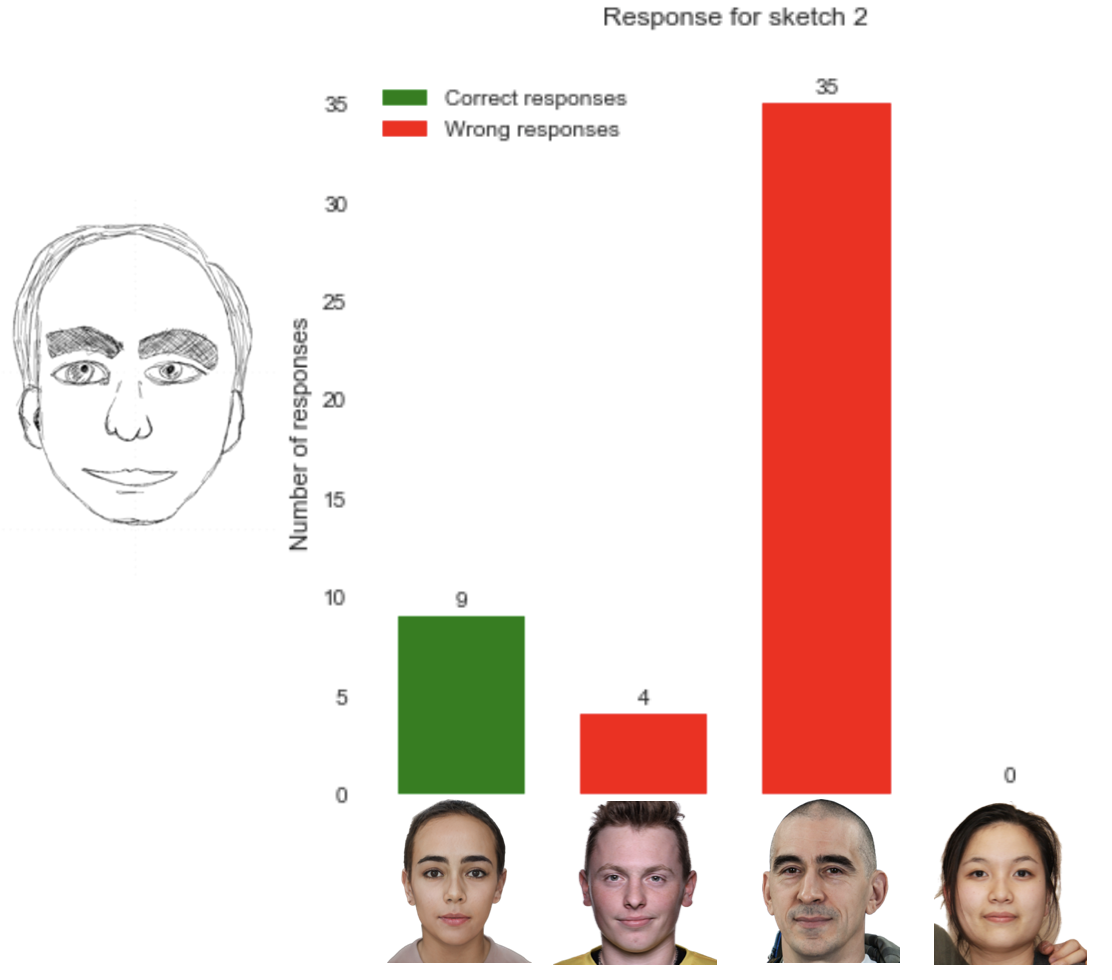
\includegraphics[width=.55\textwidth]{figures/RISULTATI/sketch2Responses.png}} \quad
    \subfloat[][\emph{}]
    {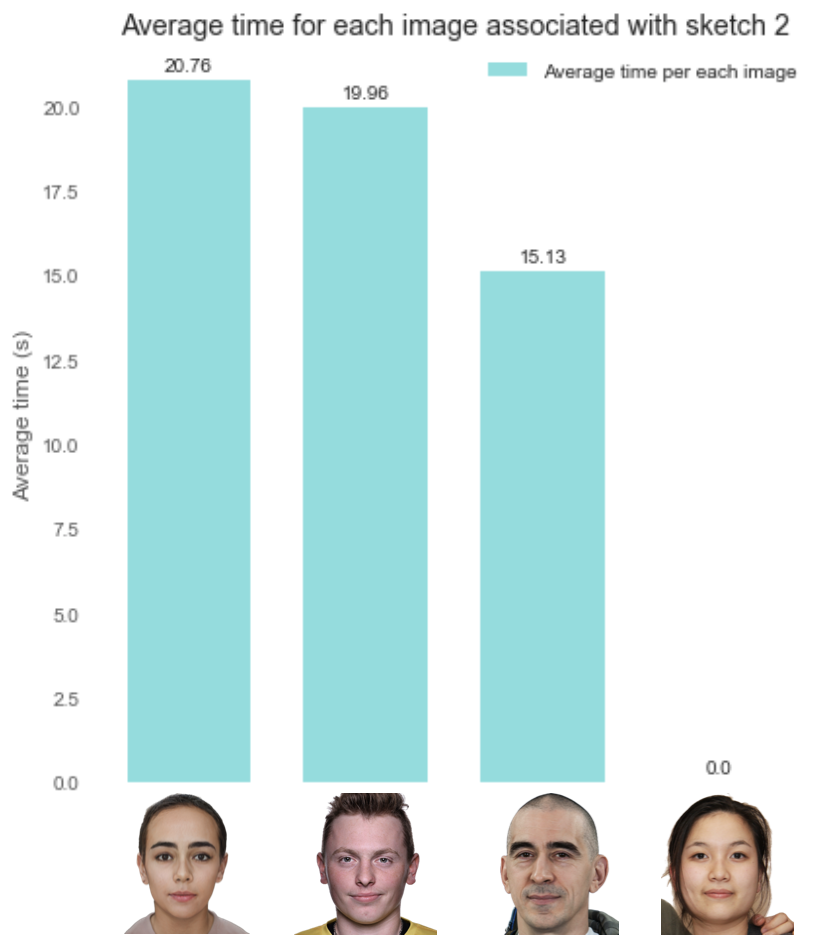
\includegraphics[width=.42\textwidth]{figures/RISULTATI/sketch2-time.png}}
    \caption{Sketch with the greatest percentage of incorrect responses}
    \label{fig:result sketch with greatest numb of incorrect}
\end{figure}

%
\noindent The results obtained for the sketch with ID \num{8} are shown in Fig.~\ref{fig:result sketch with greatest numb of correct}, where it can be observed that this sketch obtained the highest number of correct responses, most likely because the correct image was easily identifiable.

\begin{figure}[!ht]
    \centering
    \subfloat[][\emph{ }]
    {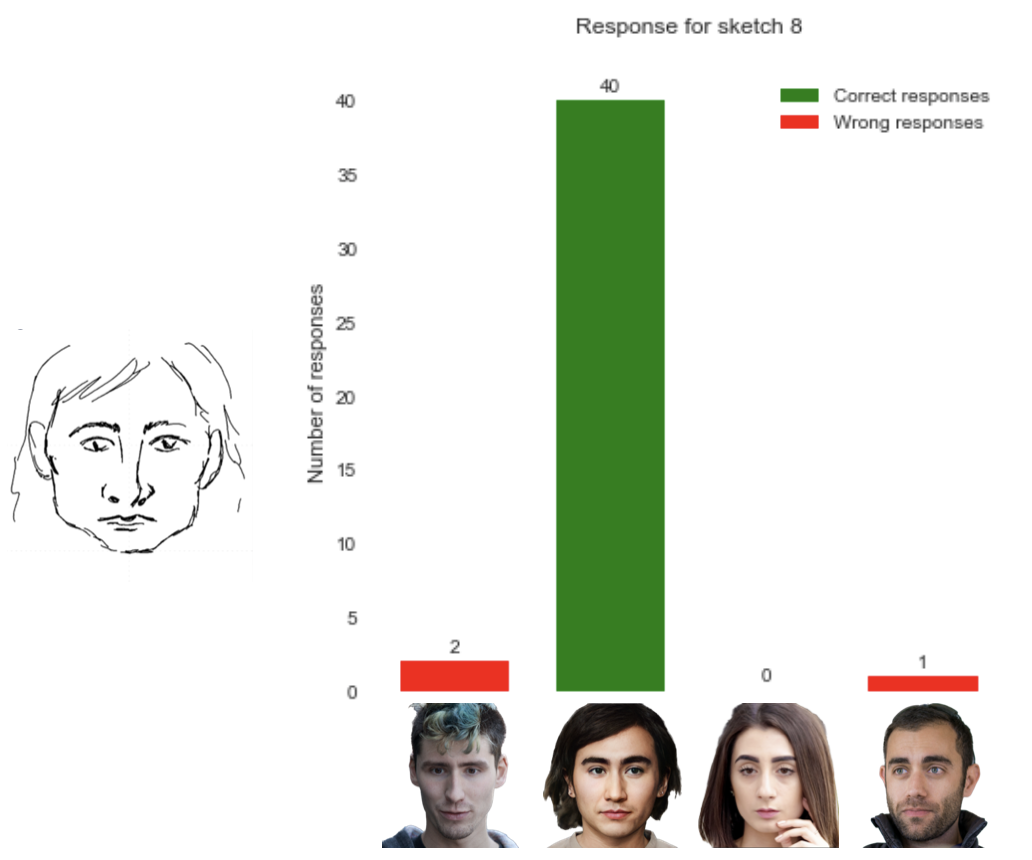
\includegraphics[width=.55\textwidth]{figures/RISULTATI/sketch8Responses.png}} \quad
    \subfloat[][\emph{}]
    {\includegraphics[width=.42\textwidth]{figures/RISULTATI/sketch8-time.png}}
    \caption{Sketch with the greatest percentage of correct responses}
    \label{fig:result sketch with greatest numb of correct}
\end{figure}

%
\noindent Looking at the average time, for almost all the images the time taken to choose a response is the same, exception made for sketch \num{19} and \num{10} that respectively obtained a lower and higher value than average time. In Figure~\ref{fig:result sketch with lowest average time}, the number of correct/incorrect responses and the average time for each similar image associated to sketch \num{19} are shown, and the same information are represented in Fig.~\ref{fig:result sketch with highest average time} for sketch \num{10}.\\
\begin{figure}[!ht]
    \centering
    \subfloat[][\emph{ }]
    {\includegraphics[width=.55\textwidth]{figures/RISULTATI/sketch19Responses.png}} \quad
    \subfloat[][\emph{}]
    {\includegraphics[width=.42\textwidth]{figures/RISULTATI/sketch19-time.png}}
    \caption{Sketch with the lowest average time}
    \label{fig:result sketch with lowest average time}
\end{figure}
\begin{figure}[!ht]
    \centering
    \subfloat[][\emph{ }]
    {\includegraphics[width=.55\textwidth]{figures/RISULTATI/sketch10Responses.png}} \quad
    \subfloat[][\emph{}]
    {\includegraphics[width=.42\textwidth]{figures/RISULTATI/sketch10-time.png}}
    \caption{Sketch with the highest average time}
    \label{fig:result sketch with highest average time}
\end{figure}

\noindent Before drawing any conclusions, it is of extreme importance to determine whether the proportion of correct answers is due to an actual understanding of the difference between the proposed images and people could actually determine which of the images was inspired by the sketch, rather than just guessing the correct answer. Therefore, the binomial test was performed, to calculate the likelihood of getting a certain number of successes, based on the assumption that the result was randomly obtained. The test essentially checks if the results are statistically significant or just due to random chance.

\noindent The null hypothesis considered in this test is that there is no significant difference between the observed proportion of success and the expected proportion of success by chance, while the p-value represents the probability of observing more extreme outcomes than the observed ones.
If the p-value is below a predetermined significance level, the null hypothesis is rejected, and it is concluded that the observed outcome is unlikely to be due to chance alone.

\noindent For each question in the survey there are four possible responses, but just one is correct, therefore the probability of guessing it correctly is \num{25}\%.
The significance value alpha is set to \num{0.05} for all tests. The null hypothesis for the test states that the proportion of correct answers is equal to \num{25}\%, while the alternative hypothesis was that the proportion was greater than \num{25}\%.

\noindent The results of the analysis, shown in Table~\ref{tab:binomial test results}, indicate that, for \num{18} out of the \num{20} questions, the p-value is less than alpha. This suggests that the percentage of correct responses is significantly higher than chance, meaning that it is unlikely that the correct responses are the result of random choices.
%
\begin{table}[!ht]
\begin{center}
    \begin{tabular}{lc}
    \textbf{SketchID} & \textbf{p-value}  \\
    0 & 0.65 \\
    1 & 0.00 \\
    2 & 0.88 \\
    3 & 0.00 \\
    4 & 0.00 \\
    5 & 0.00 \\
    6 & 0.00 \\
    7 & 0.00 \\
    8 & 0.00 \\
    9 & 0.00 \\
    10 & 0.00 \\
    11 & 0.00 \\
    12 & 0.00 \\
    13 & 0.02 \\
    14 & 0.00 \\
    15 & 0.02 \\
    16 & 0.00 \\
    17 & 0.00 \\
    18 & 0.00 \\
    19 & 0.00 \\
    \end{tabular}
     \caption{\label{tab:binomial test results}Results of the binomial test}
\end{center}
\end{table}

\noindent For the questions related to sketch \num{0} and \num{2}, the null hypothesis cannot be rejected, suggesting that the proportion of correct answer is not significantly different from chance. As can be noticed from Figure~\ref{fig:similar images sketch 0 and 2}, the images proposed for these sketches appear to be very similar, making the selection more challenging.
Overall, these findings suggest that the participants generally performed better than chance.

\noindent Furthermore, this statistical test was also performed on the overall results, considering the number of correct responses out of the total responses, that is \num{509} out of \num{775}. The p-value obtained in this case is \num{0.00}.\\
\begin{figure}[!ht]
    \centering
    \subfloat[][\emph{ }]
    {\includegraphics[width=.4\textwidth]{figures/RISULTATI/sketch0.png}} \quad
    \subfloat[][\emph{}]
    {\includegraphics[width=.4\textwidth]{figures/RISULTATI/sketch2.png}}
    \caption{Images associated with sketch \num{0} and \num{2}}
    \label{fig:similar images sketch 0 and 2}
\end{figure}

\noindent An additional analysis was conducted to examine the correlation between the response time and the accuracy of the choices made. 
In particular, the Spearman correlation coefficient was used, as it measures the strength and direction of the association between two variables. Specifically, it assesses the monotonic relationship between the two variables, meaning that it measures how well the relationship between the variables can be described by a monotonic function. 

\noindent In order to determine if such correlation exists, the two variable considered are the percentage of correct responses and the average time spent to choose the response for each sketch. The Spearman correlation coefficient obtained is \num{-0.56} with a p-value of \num{0.01}, results that indicate statistically significant negative correlation between the two variables. Therefore, as the average time spent to answer increases, the number of correct responses decreases.
Figure~\ref{fig:scatter plot relation avg time and percentage of correct responses} shows this negative correlation between the average time spent per response and the percentage of correct responses. The percentage of responses is represented on the x-axis, and the time spent per response is represented on the y-axis.

\begin{figure}[!ht]
  \centering
  \includegraphics[width=0.8\textwidth]{figures/RISULTATI/relationshipTime-responses.png}
  \caption{Scatter plot representing the relation between the average time and the percentage of correct responses}
  \label{fig:scatter plot relation avg time and percentage of correct responses}
\end{figure}

\noindent A further test was conducted during the process of collecting sketches, mentioned earlier in this chapter, several people expressed their curiosity in testing the model's capability to generate an image of the most dreamt person in the world as claimed by many people since 2006.
The phenomenon was called “This Man” and it also has a dedicate website where people experiences are collected and shared, including the description of this man.
Given the interest and the curiosity generated, the GAN model was used to attempt to produce the image corresponding to the man sketch. By feeding the sketch of this famous man into the trained model, the objective was to generate a visual representation of this person. The resulting image is illustrated in Figure~\ref{fig:this man output}, and it reveals the face of a woman maintaining the primary facial characteristics of the original sketch.

\begin{figure}[!ht]
  \centering
  \includegraphics[width=0.8\textwidth]{figures/RISULTATI/thisMan-output.png}
  \caption{Sketch of the most dreamt man and its corresponding generated image}
  \label{fig:this man output}
\end{figure} % CAP 6
\newpage
\section{Conclusions}
\label{sec:conclusion} % CAP 7

\newpage
\bibliographystyle{plain}
\bibliography{bibliografia}
%\bibliography{plain.bst}

%\printbibliography
\end{document}
